\bookpart{表示}{Representation}
\label{part:pgm-representation}

\BookPartGuide{%
概率图模型同时表示一组随机变量的联合分布和变量之间的条件独立。直接列出高维联合分布需要指数级参数，也难以看出哪些局部关系能够支持推断。本部分围绕同一个问题展开：怎样用图和局部因子保留回答查询所需的依赖，同时避免把偶然的参数关系误当作结构性质。

第~\ref{chap:pgm-overview}章“概率图模型概述”从设备诊断和温度预测进入，先区分点预测与结构化分布，再介绍有向边、无向边、观测节点、参数、重复框和因子节点的读图方式，并给出推断、学习与历史方法的整体路线。第~\ref{chap:pgm-directed}章“有向图模型”用条件分布乘积建立有向无环图，重点说明父集、条件独立、d-分离、Markov毯以及局部因子如何推出联合分布。第~\ref{chap:pgm-undirected}章“无向图模型”改用团上的非负势和全局配分函数表示对称相容关系，比较局部、成对和全局Markov性质。第~\ref{chap:pgm-representations}章“图表示的转换与因子图”处理道德化、弦化、完美映射和因子图，把结构转换、独立性集合与局部函数重组分开核对。

阅读本部分时，应同时追踪三个层次：分布的概率值是否保持，图能够保证哪些条件独立，以及局部因子怎样组织成后续可计算的形式。同一分布可以有不同图表示；某种表示少读出独立性，并不必然改变它所表示的联合分布。}

\chapter{概率图模型概述}
\label{chap:pgm-overview}

一台设备发出报警，维修人员需要判断是否停机检查。设备故障造成的过热和传感器失灵都可能触发报警，因此同一条报警记录可以对应不同的内部状态。判断“有故障”之外，还需要估计故障发生的概率，并结合后续温度读数更新判断。故障概率为$0.02$与$0.45$时，即使模型给出同一个分类结果，停机决策所依据的风险也不同。

设备诊断因而需要一个同时描述故障、温度与报警的分布。\term{概率图模型}（probabilistic graphical model, PGM）将这些随机变量画成节点，用图组织局部依赖，再由局部概率函数组成联合分布。可信的局部依赖假设可以减少需要指定的概率，也为复用计算提供依据。本章沿着设备诊断展开：先说明分布保留了哪些预测信息，再建立图与联合分布的关系，最后区分根据证据查询概率和根据数据确定模型这两类任务。

\section{从单值预测到结构化分布}
\label{sec:pgm-overview-distribution-prediction}

以传感器读数$x$预测设备下一时刻的温度时，模型可以返回$\hat y=f(x)$。这种\term{点预测}（point prediction）用一个数值概括输出，分类任务则用一个类别概括输出。它能直接进入后续决策，但单个结果中包含的信息有限，例如一个温度均值没有说明高温状态出现的概率。

保留这些信息的一种方式是给出\term{预测分布}（predictive distribution）$p(y\mid x)$，描述输入固定后各个输出的可能性。离散输出由每种结果的概率表示，连续输出由概率密度表示，落入某个区间的概率通过积分得到。分布可以同时呈现结果的集中位置、分散程度和多个分离的高概率区域。

图~\ref{fig:pgm-overview-predictive-density}用一个人工设定的温度分布说明这种区别。冷却系统有两种可能工况，预测密度分别集中在$40\,^\circ\mathrm{C}$和$80\,^\circ\mathrm{C}$附近，权重各为一半。两种工况的平均温度是$60\,^\circ\mathrm{C}$，恰好落在两个峰之间的低密度区域。保留完整分布能够同时呈现高温和低温工况；用均值或其中一个峰作点预测，则分别丢失峰的位置或另一种工况的信息。

\begin{figure}[htbp]
  \centering
  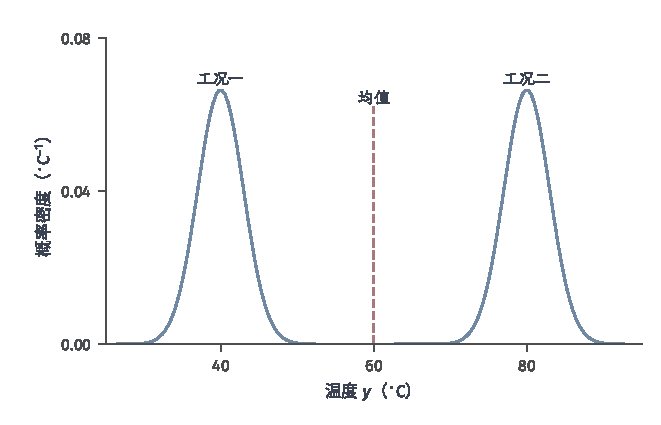
\includegraphics[width=105.412mm]{figures/06-probabilistic-graphical-models/01-representation/matplotlib/pgm-overview-predictive-density/figure.pdf}
  \caption{温度预测中的双峰分布与均值。实线为两个等权高斯密度的混合，每个分量的标准差为$3\,^\circ\mathrm{C}$；虚线标出均值$60\,^\circ\mathrm{C}$。两种工况集中在均值两侧，因而均值这一点预测省略了高概率区域的位置。图中分布为教学设定。}
  \label{fig:pgm-overview-predictive-density}
\end{figure}

预测分布也可以用来产生点预测。设备控制需要一个温度设定值时，可以从分布中选择均值；判断最可能工况时，可以选择概率最大的结果；停机决策则需要把可能的损失一并考虑。分布保留输出的不确定性，具体任务决定怎样将这些信息转化为数值、类别或行动。

当设备包含多个相互影响的部件时，预测还需要联合描述它们的状态。$d$个二值变量共有$2^d$种状态组合，直接指定完整联合表需要$2^d-1$个自由参数。变量数量增加会使数据分散在更多组合中，边缘概率的计算也可能涉及大量状态的汇总。利用局部依赖组织联合分布，正是为了在假设允许的范围内减少参数和计算。

故障与报警之间的联系必须保留，因而把所有变量设为相互独立会损失诊断所需的信息。局部简化可以更有针对性：假设报警只直接依赖过热和传感器失灵，那么给定这两个状态后，故障状态便不再改变报警的局部概率。这种“给定哪些状态后，另一个状态不再提供额外信息”的关系由条件独立表达，并由图结构记录。

\section{图模型上的表示}
\label{sec:pgm-overview-representation}
\label{sec:pgm-overview-basic-concepts}

设备诊断需要同时记录故障、过热、报警和传感器状态。画成图以后，读者不仅要知道哪些状态有关，还要分清哪些量已经观测、哪些量需要推断，以及哪些数值只是模型给定的参数。本节参考PRML第8章的图表示约定，用同一个设备例子说明节点、连线和重复框的含义\scite{bishop2006}。

\paragraph{随机变量与观测状态}
为设备的四种状态分别引入二值随机变量：故障$F$、过热$H$、报警$A$和传感器失灵$S$。每个变量取值$1$表示相应事件发生，取值$0$表示未发生。大写字母表示随机变量，小写$f,h,a,s\in\{0,1\}$表示它们的具体取值；因此$p(f,h,a,s)$是$F=f,H=h,A=a,S=s$同时成立的概率。

圆圈表示随机变量，圈内写变量名称。节点也可以代表一个随机向量，例如把四种状态合为$\bm V=(F,H,A,S)$，图中便可只画一个标有$\bm V$的圆圈。图~\ref{fig:pgm-overview-node-granularity}比较这两种粒度：圆圈的数量并不一定等于标量分量的数量。对于当前尚未取得取值的变量，节点保持空心；已经观测到的变量则给圆圈填色。只有报警记录$A=1$时，$A$画成填色圆圈，$F,H,S$仍为空心。若随后测得过热状态，$H$也改为填色，但模型中的依赖关系不必因此改变。图~\ref{fig:pgm-overview-visual-conventions}对照这两个观测条件，连线保持不变，变化的是节点的填色。

\begin{figure}[!htb]
  \centering
  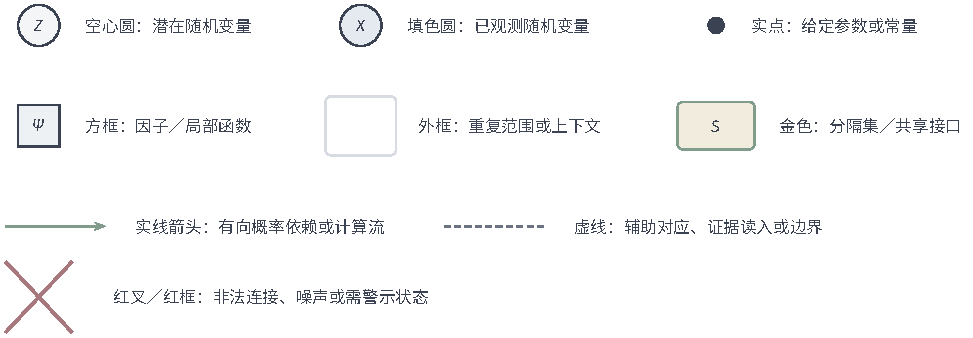
\includegraphics[width=77.646mm]{figures/06-probabilistic-graphical-models/01-representation/tikz/pgm-overview-visual-conventions/figure.pdf}
  \caption{观测信息改变节点填色。(a)仅知报警$A=1$；(b)又测得过热$H=1$。两图使用相同的变量与连线，故障和传感器状态仍未观测；填色表示已有取值，不表示删除随机变量。}
  \label{fig:pgm-overview-visual-conventions}
\end{figure}
\FloatBarrier

\begin{figure}[!htb]
  \centering
  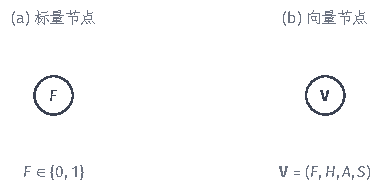
\includegraphics[width=64.703mm]{figures/06-probabilistic-graphical-models/01-representation/tikz/pgm-overview-node-granularity/figure.pdf}
  \caption{圆圈可以表示不同粒度的随机量。(a)一个故障状态$F$；(b)由四种状态组成的随机向量$\bm V$。向量节点并没有把四个分量变成同一个标量，也不表明各分量独立。}
  \label{fig:pgm-overview-node-granularity}
\end{figure}
\FloatBarrier

填色说明这次查询已知什么，不改变变量原本的随机性。空心也不专指模型主动引入的潜变量：尚未观测的故障是当前诊断目标，未来尚未产生的报警也可以是预测目标。对当前记录，模型引入而没有直接观测的内部状态称为潜变量；哪些节点已知、哪些未知，应结合观测条件来读。

只有报警已知而要判断故障时，必须先汇总过热和传感器失灵的可能取值，再按报警概率归一化：
\begin{equation}
  p(f,a)=\sum_{h,s}p(f,h,a,s),
  \qquad
  p(f\mid a)=\frac{p(f,a)}{p(a)},\quad p(a)>0.
  \label{eq:pgm-overview-marginal-conditional}
\end{equation}
这里$\sum_{h,s}$遍历$h,s\in\{0,1\}$的四种组合，$p(a)=\sum_f p(f,a)$；竖线右侧的$a$是已经给定的报警取值。第一式得到故障与报警的边缘概率，第二式使给定报警后故障两种取值的概率之和为$1$。连续变量用相应积分消去，条件分布的基本约定见\BookSectionRef{sec:rv-conditional-distribution}{卷2《数学准备：概率、因果与决策》第1章“随机变量”第1.2.2.2节“条件信息下的分布关系”}。

\paragraph{有向边与局部条件分布}
节点说明模型包含哪些量，连线则组织这些量之间的关系。先不省略任何条件，链式法则给出
\[
  p(f,s,h,a)=p(f)p(s\mid f)p(h\mid f,s)p(a\mid f,s,h).
\]
每一项都保留之前变量的全部取值，因此这种写法并没有减少完整联合表所需的参数。只有进一步指定条件独立关系，才能删去不需要的条件。

条件独立记为$X\perp Y\mid W$，其中$X,Y,W$是随机变量，$x,y,w$是它们各自的取值：给定$W$后，再知道$Y$不会改变$X$的条件分布。对本节的离散变量，在$p(y,w)>0$时可写为$p(x\mid y,w)=p(x\mid w)$；一般条件分布的等式按条件变量的分布几乎处处成立。当前需要的是这些关系怎样简化局部函数，通用独立性约定可参考\BookSectionRef{sec:probability-moments-independence}{卷2《数学准备：概率、因果与决策》第1章“随机变量”第1.2.3节“随机变量的独立关系”}。

设备模型假设故障与传感器失灵独立，过热在给定故障后不再依赖传感器状态，报警在给定过热与传感器状态后不再依赖故障。由此将链式分解中的相应条件删去，得到
\begin{equation}
  p(f,h,a,s)=p(f)p(s)p(h\mid f)p(a\mid h,s).
  \label{eq:pgm-overview-device-joint}
\end{equation}
每个局部条件分布对输出变量归一化，这个乘积就定义了完整联合分布。二值根变量$F,S$各需一个参数；$H$在$F$的两个取值下各需一个参数；$A$在$(H,S)$的四种组合下各需一个参数。总计$8$个自由参数，而完整联合表需要$15$个；减少的参数来自这里采用的独立性假设。

\term{有向图模型}（directed graphical model）用箭头指定局部条件分布使用哪些父变量。进入$A$的两条边$H\to A\leftarrow S$对应$p(a\mid h,s)$；$F\to H$对应$p(h\mid f)$；没有进入$F,S$的边，所以它们分别使用$p(f),p(s)$。图~\ref{fig:pgm-overview-device-graph}画出这一对应。箭头先表示概率分解中的条件关系，因果解释需要额外假设；它也不表示算法必须按箭头方向传递查询信息。第~\ref{chap:pgm-directed}章进一步说明有向分解与条件独立的对应。



\begin{figure}[!htb]
  \centering
  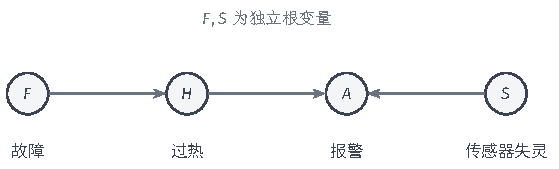
\includegraphics[width=94.590mm]{figures/06-probabilistic-graphical-models/01-representation/tikz/pgm-overview-device-graph/figure.pdf}
  \caption{设备诊断的有向表示。节点表示随机变量，进入节点的箭头指定其局部条件分布所依赖的变量，例如$H\to A\leftarrow S$对应$p(a\mid h,s)$。这里的箭头记录概率分解，因果解释需要另行给出假设。}
  \label{fig:pgm-overview-device-graph}
\end{figure}

\FloatBarrier

\paragraph{固定量与参数节点}
图规定局部函数可以使用哪些变量，函数中的数值还需另外指定。例如，令$\bm\theta_A$收集四种$(h,s)$组合下的报警概率$p(A=1\mid H=h,S=s)$。查询故障时，若这张概率表已经给定，$\bm\theta_A$就是固定量，可以画成小实点，再连到使用它的报警节点。图~\ref{fig:pgm-overview-parameter-roles}(a)只保留报警与其固定参数，显示小实点的作用。

填色大圆圈与小实点承担不同职责：前者是模型中的随机变量，只是本次已经取得取值；后者在当前概率模型中作为给定量使用，不需要对它建立概率分布。固定输入也可以用小实点表示，例如回归中给定的输入位置。参数是否画成实点取决于建模方式，而不是它被称为“参数”：若要为参数本身指定先验并推断其分布，就应将它画成随机变量圆圈。图~\ref{fig:pgm-overview-parameter-roles}(b)用$\bm\Theta_A$表示随机参数，$\bm\theta_A$仍表示它的一种取值。具体参数学习方式由第~\ref{chap:pgm-parameter-learning}章介绍。

\begin{figure}[!htb]
  \centering
  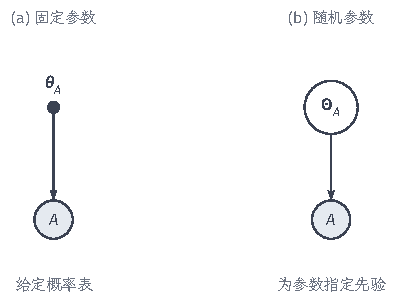
\includegraphics[width=67.165mm]{figures/06-probabilistic-graphical-models/01-representation/tikz/pgm-overview-parameter-roles/figure.pdf}
  \caption{同一参数的两种建模方式。左图将报警表作为固定量，右图为参数$\bm\Theta_A$指定先验，使用随机变量圆圈。两图都观测报警$A$，均省略$H,S$及其入$A$的箭头；实点与填色圆圈不是同一类对象。}
  \label{fig:pgm-overview-parameter-roles}
\end{figure}
\FloatBarrier

同一张图配上不同的局部概率表，会给出不同的诊断结果。图结构组织允许的依赖，参数与局部函数确定具体概率；为保持图简洁，已经在正文说明的固定参数可以不全部画出。

\paragraph{重复框与共享参数}
多台设备采用相同诊断模型时，每条记录都有自己的$F_i,H_i,A_i,S_i$。若逐条画出，节点和连接会大量重复。\term{板表示法}（plate notation）用一个框圈住代表性节点及其连接，再用$N$标出重复次数；下标$i=1,\ldots,N$说明框内变量按记录复制。图~\ref{fig:pgm-overview-plate-expansion}取$N=3$对照展开图和板框图，只保留过热、传感器失灵与报警这三个节点；省略的故障节点也随记录复制。框外的$\bm\theta_A$不复制，而是由每套报警节点共同使用。

\begin{figure*}[!htb]
  \centering
  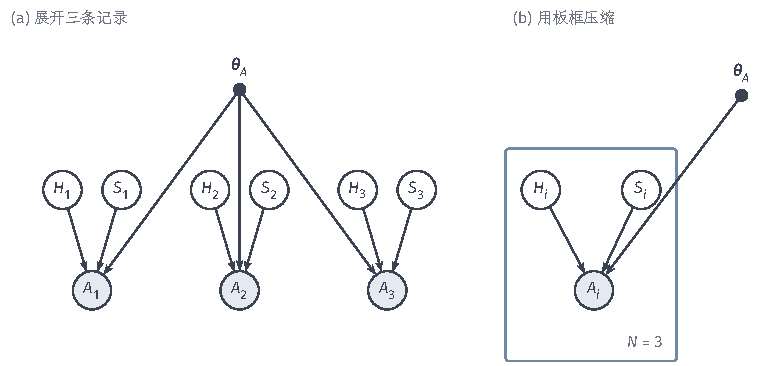
\includegraphics[width=128.926mm]{figures/06-probabilistic-graphical-models/01-representation/tikz/pgm-overview-plate-expansion/figure.pdf}
  \caption{重复框与展开图，取三条记录作图示。左图有三个过热、三个传感器和三个报警变量，三组报警共用一个固定参数；右图用$N=3$的板框压缩这些副本。两图均省略故障变量及相关箭头，框外参数不随记录复制。}
  \label{fig:pgm-overview-plate-expansion}
\end{figure*}
\FloatBarrier

若各记录在给定整组固定参数$\bm\theta$后相互独立，用$p_{\bm\theta}$表示采用这组参数的分布，则重复图对应的联合概率为
\begin{equation}
  p_{\bm\theta}(f_{1:N},h_{1:N},a_{1:N},s_{1:N})
    =\prod_{i=1}^{N}p_{\bm\theta}(f_i,h_i,a_i,s_i).
  \label{eq:pgm-overview-plate-product}
\end{equation}
$\bm\theta$包含四类局部概率表的全部参数，$f_{1:N}$表示$f_1,\ldots,f_N$，其余下标同理。每条记录使用相同的函数形式和参数，但保留自己的状态取值。框本身只表示重复，不单独保证记录独立；若副本之间另有连接，或共享的随机量被边缘化，就要按展开后的依赖关系计算联合分布。

\paragraph{无向边与因子节点}
若重点是邻近部件状态之间的对称相互作用，可以使用\term{无向图模型}（undirected graphical model）。无向边没有箭头，不指定哪个端点作为另一个端点的条件；局部关系由非负势函数评价配置的相对权重。令$\bm x$为全部变量的取值，$c$为局部作用范围的索引，$\bm x_c$为该范围内的取值子向量，则
\[
  p(\bm x)=\frac{1}{Z}\prod_c\psi_c(\bm x_c),
  \qquad
  Z=\sum_{\bm x}\prod_c\psi_c(\bm x_c).
\]
$\psi_c\geq0$是局部势，$Z$是对全部候选配置求和的归一化常数。离散情形下$p(\bm x)$表示联合概率，连续情形下表示密度；连续状态改用积分，且须满足$0<Z<\infty$。无向边表示模型允许的局部相互作用，不等同于两个变量的边缘相关系数。其条件独立语义在第~\ref{chap:pgm-undirected}章展开。

局部函数也可以单独画出来。\term{因子图}（factor graph）用圆圈表示变量、方框表示因子，连接线说明函数用到了哪些变量。例如，令$g_A(a,h,s)=p(a\mid h,s)$，相应的$g_A$方框连接$A,H,S$。这三条无箭头连线表示函数的三个自变量，并不是新增三条随机变量之间的无向边；$g_A$也不需要被观测或赋予一个随机取值。图~\ref{fig:pgm-overview-edge-types}进一步对照无向变量边和一个三变量因子的连线：左图直接连接变量，右图把局部函数单独画出。

\begin{figure}[!htb]
  \centering
  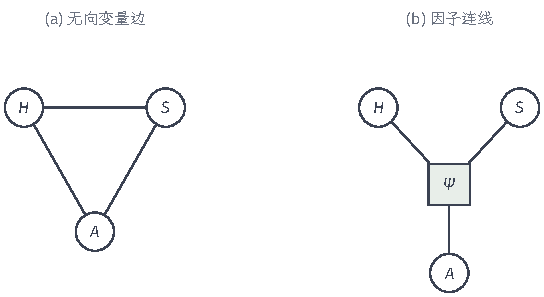
\includegraphics[width=92.135mm]{figures/06-probabilistic-graphical-models/01-representation/tikz/pgm-overview-edge-types/figure.pdf}
  \caption{无向边与变量—因子连线的对象不同。左图允许$H,S,A$组成一个三变量局部作用范围，右图将该范围的势函数$\psi(h,s,a)$显式画成方框。右图的每条线连接一个变量和一个函数，不能读成新增的变量之间连线；两图均不标注观测证据。}
  \label{fig:pgm-overview-edge-types}
\end{figure}
\FloatBarrier

有向模型的条件概率乘积和无向模型的势函数乘积都能画成因子图。圆圈与方框的区别使每个乘积项的作用范围显式可见；原来的父子方向则要由局部函数的含义说明。因此，因子图提供的是乘积分解的计算表示，第~\ref{chap:pgm-representations}章将比较不同表示保留的信息。

算法图中的消息箭头、辅助虚线、分隔集色框和警示颜色由相应图注说明；它们不属于上述概率图节点与边的通用语义，不能只凭颜色或线型判断模型含义。

\FloatBarrier

\section{图模型上的推断与学习}
\label{sec:pgm-overview-inference-learning}

报警记录提出的查询是$p(F=1\mid A=1)$。在图结构和局部概率已知时，根据证据计算这种查询称为\term{概率推断}（probabilistic inference）。过热$H$和传感器状态$S$仍然未知，所以推断要把它们可能处于的每一种状态都纳入后验计算。

为观察计算量如何变化，将诊断范围扩展到更多部件，并设共有$30$个未观测的二值状态，包括$H,S$以及新增的部件或运行状态。将它们统一记为$\bm{Z}=(Z_1,\ldots,Z_{30})$，仍以报警$A=1$为证据、故障$F$为查询目标。后验的分子汇总故障发生时的未知配置，分母汇总故障两种取值下的配置：
\begin{equation}
  p(F=1\mid A=1)
  =
  \frac{
    \displaystyle\sum_{\bm{z}\in\{0,1\}^{30}}
    p(F=1,A=1,\bm{z})
  }{
    \displaystyle\sum_{f\in\{0,1\}}
    \sum_{\bm{z}\in\{0,1\}^{30}}
    p(f,A=1,\bm{z})
  }.
  \label{eq:pgm-overview-expanded-diagnosis}
\end{equation}
直接展开该式时，分子包含$2^{30}$个未观测状态配置，约为$10.7$亿项；分母同时遍历故障的两个取值，包含$2^{31}$个完整配置项，约为$21.5$亿项。这是对状态组合的计数，所需模型参数仍由局部函数决定。

对于一个完整配置$p(f,A=1,\bm{z})$，局部分解允许逐项查表或计算，再将结果相乘。后验却要汇总许多这样的配置，因此主要开销可能来自求和，而非单次乘积评价。若不同配置共享某些局部计算，图结构便可能帮助复用这些结果；复用范围和中间结果大小取决于变量之间的连接方式。

\term{精确推断}（exact inference）重组概率运算，在给定模型下求出原查询的准确答案，其时间和空间开销受问题规模及中间结果大小影响。预算不足以容纳这些中间计算时，可以采用\term{近似推断}（approximate inference），在可承受的时间或空间内估计查询，并分析所引入的误差。第~\ref{chap:pgm-elimination}章至第~\ref{chap:pgm-sampling}章分别讨论这些计算方法及其适用结构。

设备运行记录可以用来确定局部概率的数值。例如，在故障和过热状态均被记录时，故障设备中过热的比例可以用于估计$p(H=1\mid F=1)$。在图结构和局部函数形式给定的前提下估计这些数值，称为\term{参数学习}（parameter learning）。稀有状态只有少量样本时，估计受随机波动影响较大；存在缺失或潜变量时，还需要处理无法直接取得的状态计数。

若设备内部哪些状态应当直接相连也未知，就需要根据数据和领域约束选择图，这称为\term{结构学习}（structure learning）。增加连接可以描述更多依赖，通常也会扩大局部函数并增加估计和推断的开销；减少连接则需要确认相应独立性假设是否适合数据。学习所得的有向结构首先描述概率关系，因果解释仍取决于额外假设和证据。

这两类学习任务确定模型，而推断利用给定模型计算未知状态的概率。含有未观测变量的数据将二者联系起来：参数更新所需的统计量可能依赖潜在状态，于是先用当前模型计算这些状态的后验，再据此更新参数。第~\ref{chap:pgm-parameter-learning}和第~\ref{chap:pgm-structure-learning}章将分别展开参数估计与结构选择。

\section{概率图模型的历史}
\label{sec:pgm-overview-history}

局部相互作用如何组成整体分布，观测如何改变未知状态的概率，未知参数又如何从数据中估计，这些问题推动了概率图模型的发展。图~\ref{fig:pgm-overview-history}与图~\ref{fig:pgm-overview-history-recent}按时间展示代表工作，以下结合各自处理的计算与建模问题说明它们的联系。

\begin{figure*}[p]
\centering
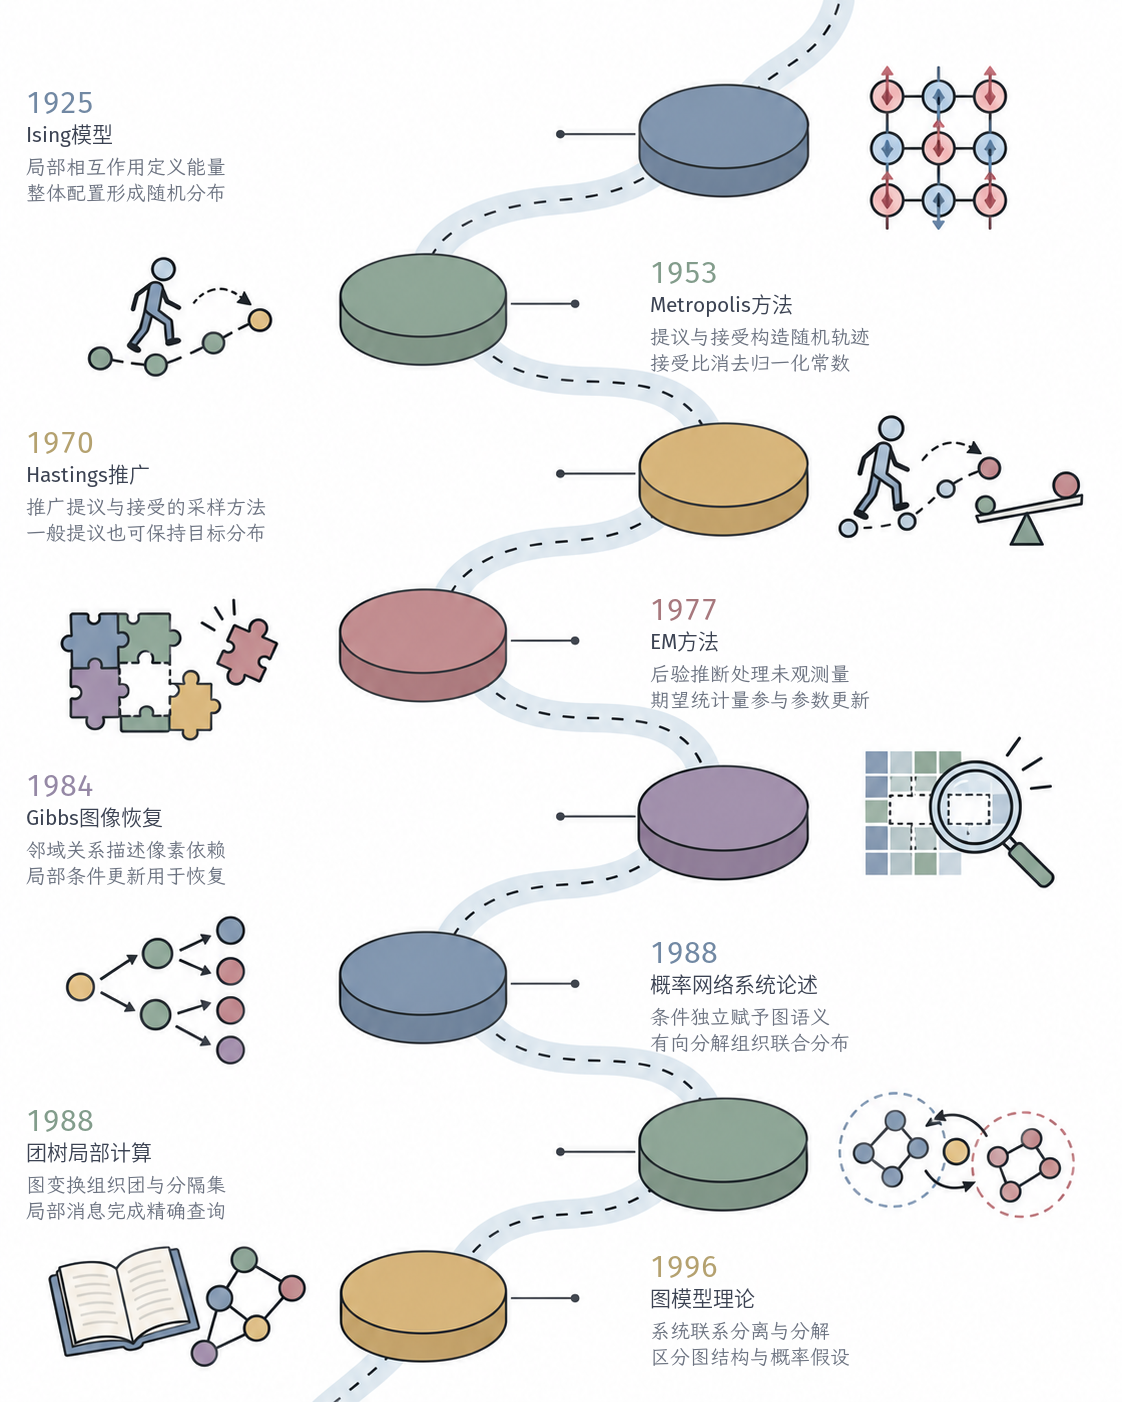
\includegraphics[width=157.406mm,height=.88\textheight,keepaspectratio]{figures/06-probabilistic-graphical-models/04-models/generated/pgm-models-history/figure.png}
\caption{概率图模型发展的代表工作（1925—1996）。沿虚线路线从上向下阅读：局部相互作用组织联合分布，随机更新估计难以直接计算的查询，潜变量学习处理缺失状态，图语义与消息计算联系独立性和推断。1988年Pearl的节点对应系统论述，而非概率网络的首次提出；节点间距不按时间比例绘制。}
  \label{fig:pgm-overview-history}
\end{figure*}
\begin{figure*}[p]
\centering
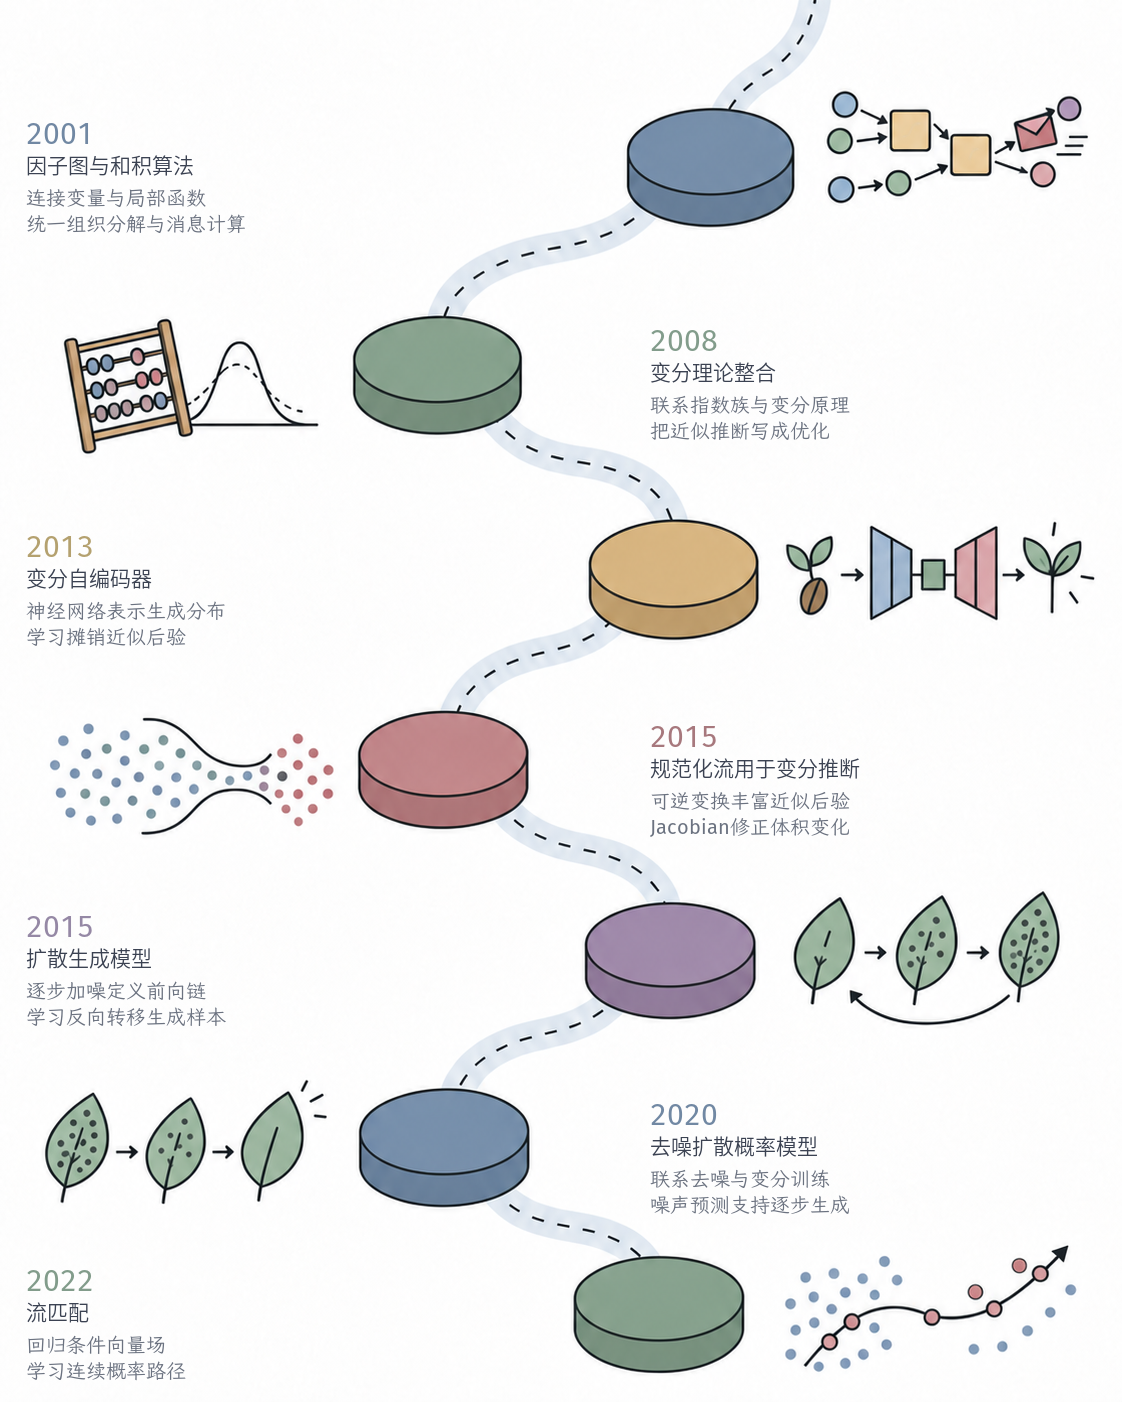
\includegraphics[width=157.406mm,height=.88\textheight,keepaspectratio]{figures/06-probabilistic-graphical-models/01-representation/generated/pgm-models-history-recent/figure.png}
\caption{概率图模型发展的代表工作（2001—2022），承接图~\ref{fig:pgm-overview-history}。因子图组织局部函数与消息，变分理论统一近似推断的优化表述，神经参数化进一步扩展后验近似和生成路径。2008年对应理论整合工作，2015年的规范化流对应流式变分推断；年份采用代表文献的首次公开或发表时间，不表示各类方法的统一起点。}
  \label{fig:pgm-overview-history-recent}
\end{figure*}

\subsection{从局部随机规律到图结构语义}

1925年的Ising模型以相邻自旋的相互作用描述整体配置，是无向局部随机模型的早期代表。每个局部项只涉及少量自旋，而归一化常数与边缘概率仍涉及整体状态的汇总。另一类问题来自数据中的未观测变量：1977年的EM方法利用当前模型推断相关统计量，再让这些统计量参与参数更新\scite{pgm-overview-ising1925,pgm-overview-dempster1977}。

归一化常数难以直接求出时，状态更新提供了另一条计算路线。1953年的Metropolis方法及1970年的Hastings推广通过提议候选状态与决定是否接受，构造随机轨迹；接受比中共同的未知归一化常数可以消去。由轨迹估计查询的效率还取决于链能否充分探索不同状态。1984年的Geman与Geman将局部相互作用定义的Gibbs分布与随机更新用于图像恢复，使局部依赖同时参与分布描述和状态计算\scite{pgm-history-metropolis1953,pgm-history-hastings1970,pgm-history-geman1984}。

1988年Pearl对概率网络的系统论述将条件独立与有向分解联系起来。同年Lauritzen与Spiegelhalter通过图变换组织局部消息，形成一般网络上的精确计算方法；1996年Lauritzen进一步系统整理图模型理论。这些工作分别为概率分解的合法性和查询的计算方式提供依据，而具体查询的开销仍由图结构决定\scite{pgm-pearl1988,pgm-overview-lauritzen1988,pgm-lauritzen1996}。

% 保留小节标题与首段，避免两页历史插画夹断近似推断的说明。
\Needspace{10\baselineskip}
\subsection{学习、近似推断与神经参数化}

大规模模型中的后验计算促使近似推断进一步发展。变分方法在可计算的分布族中优化后验近似，误差与所选分布族及优化结果有关；采样方法通过随机轨迹估计查询，有限时间内的误差与链的探索和混合行为有关。Wainwright与Jordan在2008年的综述系统联系了指数族、变分原理和图上计算\scite{pgm-wainwright2008}。

2013年以来，神经网络进入了分布及推断的参数化：VAE同时表示生成分布与近似后验，规范化流以可逆变换构造密度，扩散模型学习逆转人为加入的噪声过程。各路线提供更灵活的局部函数，同时采用不同的似然评价、后验近似和样本生成方法，因此具有不同的计算代价\scite{kingma2013,pgm-overview-rezende2015,pgm-overview-sohl2015}。

\subsection{当前研究方向}

复杂观测数据需要灵活的分布，同时也需要可承受的后验计算。一类研究设计便于计算的分解，或学习由观测直接给出后验近似的摊销方法，并评价近似误差与校准。另一类研究面向高维条件生成，考察潜变量、可逆变换、扩散和连续流分别怎样表示条件分布、怎样生成样本。流匹配通过拟合条件向量场学习连续生成路径，是其中的代表方法\scite{lipman2023flowmatching}。

对于不完整、多模态或受领域约束的数据，还需检查模型假设的依赖能否由观测识别。除生成样本的质量外，也应分别评价分布表示的准确程度、参数学习的收敛性和预测概率的可靠程度。

\section{本章小结}
\label{sec:pgm-overview-summary}

设备诊断既要判断状态，也要估计状态的概率。联合分布保留了状态间的依赖，却增加了参数和计算量。概率图模型用条件独立假设组织局部函数，并据此简化分布表示与查询计算。

有向图通过局部条件分布分解联合概率，无向图通过势函数乘积与全局归一化表示联合概率，因子图则呈现选定的局部乘积。推断在给定模型下计算概率查询，开销取决于图结构；参数学习与结构学习根据数据确定模型，潜变量使学习与推断相互联系。

下一章从有向图出发，说明条件独立与联合分解的关系。

\paragraph{扩展阅读}
Bishop的PRML第8章解释概率分解与图表示的对应；Koller与Friedman的教材进一步展开表示、推断和学习及其计算结构\scite{bishop2006,pgm-koller2009}。

\chapter{有向图模型}
\label{chap:pgm-directed}

设备报警可以为故障提供线索，传感器失灵却也可以解释同一条报警。若随后确认传感器已经失灵，故障的后验概率就可能下降。同样是增加观测，给定过热状态可以屏蔽故障与报警之间的一条联系，给定报警状态却可能让两种解释产生关联。这些变化取决于观测节点在路径上的位置，有向图为判断它们提供了规则。

本章沿用第~\ref{chap:pgm-overview}章的设备模型，先用一个固定变量顺序写出图所采用的独立性假设，再考察节点邻域及连接两组节点的路径。随后将这些关系与局部条件分布的乘积联系起来，并用离散表和连续条件分布给出可计算的模型。全局性质蕴含局部性质的图论证明随命题给出，其余跨表示证明集中在第~\ref{sec:pgm-representations-directed-proofs}节；这些结论共同说明独立性语义、联合分解和数值参数化怎样配合。

\section{有向图模型的定义}
\label{sec:pgm-directed-definition}

用四个二值随机变量表示设备状态：故障$F$、过热$H$、报警$A$和传感器失灵$S$，取值$1$表示相应状态出现。图~\ref{fig:pgm-directed-device}采用$F\to H\to A\leftarrow S$三条箭头，对应如下局部假设：过热的条件分布以故障为输入，报警的条件分布以过热和传感器状态为输入。这个结构是用于说明概率语义的人工模型，后文的数值例子也采用教学参数。

\begin{figure}[htbp]
  \centering
  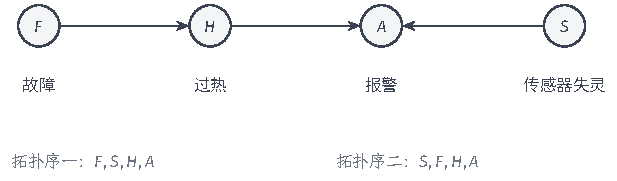
\includegraphics[width=104.482mm]{figures/06-probabilistic-graphical-models/01-representation/tikz/pgm-directed-device/figure.pdf}
  \caption{设备诊断的有向图及两个拓扑序。箭头指定局部条件分布的输入，$F$与$S$是没有父节点的根节点。下方两个序列都把父节点排在子节点之前，对应同一个图结构。}
  \label{fig:pgm-directed-device}
\end{figure}

记图为$\mathcal G=(V,E)$，其中节点对应随机变量。本部分采用有限有向无环图，并排除自环；其他结构将在使用处另行说明（相关图论约定与结论可参考\BookChapterRef{chap:graph-theory}{卷1《数学准备：计算、分析与几何》的“图的表示与计算”章}）。

局部条件分布所用的直接输入，在图中组成节点$i$的\term{父节点}（parent）集合$\operatorname{pa}(i)$；$i$直接指向的节点组成\term{子节点}（child）集合$\operatorname{ch}(i)$。将直接连接扩展为长度至少为一的有向路径，能够到达$i$的节点组成\term{祖先}（ancestor）集合$\operatorname{an}(i)$，从$i$能够到达的节点组成\term{后代}（descendant）集合$\operatorname{de}(i)$，两者都排除$i$自身。在设备图中，$\operatorname{pa}(A)=\{H,S\}$、$\operatorname{an}(A)=\{F,H,S\}$，而$\operatorname{de}(S)=\{A\}$。这些例子用变量名标记节点，一般公式则用$A\subseteq V$表示节点集合、用$\bm{X}_A$表示相应随机向量。

按顺序指定条件分布时，父节点必须先于子节点出现。有限有向无环图总能找到这样的拓扑序，而且可能有多个；图~\ref{fig:pgm-directed-device}中的$F,S,H,A$和$S,F,H,A$便是两个例子。

固定其中一个拓扑序，并将节点按该序重标记为$1,\ldots,d$。在处理节点$i$时，已经出现的节点组成\term{前驱集合}（predecessor set）$\operatorname{pre}(i)=\{1,\ldots,i-1\}$。父节点属于前驱集合，其他前驱则可能只是排在前面，例如互不相连的两个节点仍有先后次序。因此，当前顺序提供的全部条件与局部分布实际采用的父节点条件，需要分别记录。

\begin{definition}[有序Markov假设与有向图模型]
  \label{def:pgm-directed-ordered}
  给定有向图$\mathcal{G}$及一个固定拓扑序，若联合分布$p$对每个$i\in V$满足
  \begin{equation}
    X_i\perp
    \bm{X}_{\operatorname{pre}(i)\setminus\operatorname{pa}(i)}
    \mid\bm{X}_{\operatorname{pa}(i)},
    \label{eq:pgm-directed-ordered}
  \end{equation}
  则称它满足该顺序下的\term{有序Markov假设}（ordered Markov assumption）。\term{有向图模型}（directed graphical model）是有向图及其节点随机变量的联合分布，其中该联合分布满足上述假设。文献中传统上也称这类模型为\term{贝叶斯网络}（Bayesian network）；本书统一使用“有向图模型”。
\end{definition}

式~\eqref{eq:pgm-directed-ordered}将前驱中的父节点与其余节点分开：父节点给定后，其余前驱不再改变$X_i$的条件分布。这里约束的是整个分布，而均值或相关系数只描述它的部分特征。父集为空的根节点省去条件，前驱也为空时则没有需要约束的其他变量。设备顺序$F,S,H,A$中的非平凡假设写为
\[
  S\perp F,\qquad H\perp S\mid F,\qquad A\perp F\mid(H,S).
\]
这些假设当前针对选定的顺序。后面的因子分解等价关系将说明，由一个拓扑序得到的模型也满足其他合法拓扑序下的有序性质，因此所定义的模型类与具体拓扑序无关。完整证明见第~\ref{sec:pgm-representations-directed-proofs}节。

$p$表示相对于坐标参考测度乘积的联合质量或密度，条件分布等式按条件变量的分布几乎处处成立。后文用有限离散求和展示计算，密度情形在相应条件下采用积分，有向模型的结论允许联合分布取零值（条件分布及独立性的概率依据参见\BookSectionRef{sec:rv-conditional-distribution}{卷2《数学准备：概率、因果与决策》第1章“随机变量”第1.2.2.2节“条件信息下的分布关系”}与\BookSectionRef{sec:probability-moments-independence}{卷2《数学准备：概率、因果与决策》第1章“随机变量”第1.2.3节“随机变量的独立关系”}）。

有向边为局部条件分布指定可用的输入，具体参数决定该输入是否实际改变输出分布。用$F$预测$H$描述的是观测条件下的分布，主动改变$F$后的结果则需要干预语义。第~\ref{chap:pgm-structure-learning}章将讨论赋予有向结构因果解释所需的假设与识别条件。

\section{有向图的局部独立性}
\label{sec:pgm-directed-local}

给定父节点以后，哪些其他节点可以从$X_i$的条件中省去？前驱集合只能回答一个固定顺序内的问题，而图上的非后代集合可以摆脱排列。将节点自身与全部后代排除，记为
\[
  \operatorname{nd}(i)=V\setminus\bigl(\{i\}\cup\operatorname{de}(i)\bigr).
\]
父节点属于这个集合，因为父节点若同时是后代，就会与指向$i$的边组成有向环。集合排除$i$自身，随后还要把已经作为条件的父节点从待独立的变量中分出。

\begin{definition}[局部Markov性质]
  \label{def:pgm-directed-local-markov}
  分布$p$满足有向图$\mathcal{G}$的\term{局部Markov性质}（local Markov property），是指对每个节点$i$，
  \begin{equation}
    X_i\perp
    \bm{X}_{\operatorname{nd}(i)\setminus\operatorname{pa}(i)}
    \mid\bm{X}_{\operatorname{pa}(i)}.
    \label{eq:pgm-directed-local-markov}
  \end{equation}
\end{definition}

局部Markov性质用父节点屏蔽其他非后代。后代仍可能反映当前节点的状态，例如在设备模型中给定$F$以后，报警$A$还可以为过热$H$提供观测线索。因此，式~\eqref{eq:pgm-directed-local-markov}限定独立对象为非父、非后代节点。

合法拓扑序中的前驱都属于非后代，局部性质因而可以通过边缘化无须保留的独立变量，得到有序性质。相反方向涉及更多节点：在$F,S,H,A$顺序中，有序性质给出$S\perp F$，局部性质还包括排在$S$后面的$H$，即$S\perp(F,H)$。这一步需要联合分布的因子分解与祖先边缘化，证明见第~\ref{sec:pgm-representations-directed-proofs}节。

若查询要求屏蔽所有其他变量，就还要处理后代所携带的信息。能完成这种屏蔽的一组变量称为\term{Markov毯}（Markov blanket）。有向图为节点$i$提供如下标准集合：
\begin{equation}
  \begin{aligned}
    \operatorname{mb}(i)
    ={}&\operatorname{pa}(i)\cup\operatorname{ch}(i)\\
       &{}\cup\bigcup_{j\in\operatorname{ch}(i)}
           \bigl(\operatorname{pa}(j)\setminus\{i\}\bigr).
  \end{aligned}
  \label{eq:pgm-directed-blanket}
\end{equation}
该集合同时包含父节点、子节点和子节点的其他父节点，图~\ref{fig:pgm-directed-markov-blanket}分别以$P,C,U$标示。标准集合将子节点纳入条件，以处理它们对$X_i$提供的线索；给定子节点还会打开在该处碰撞的路径，于是集合同时纳入其余父节点。给定完整集合后，毯外节点$O$与$X_i$之间的路径得到屏蔽，即使$O$在原图中与毯内变量相连。

\begin{figure}[htbp]
  \centering
  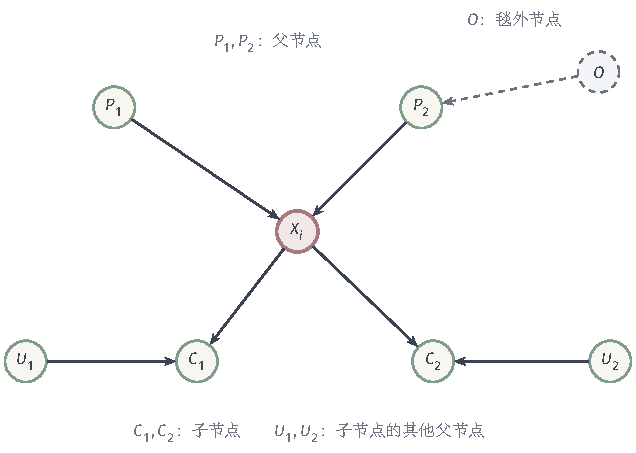
\includegraphics[width=107.685mm]{figures/06-probabilistic-graphical-models/01-representation/tikz/pgm-directed-markov-blanket/figure.pdf}
  \caption{节点$X_i$的图上Markov毯。父节点$P_1,P_2$、子节点$C_1,C_2$以及子节点的其他父节点$U_1,U_2$共同组成$\operatorname{mb}(i)$；以虚线描边的$O$位于毯外。}
  \label{fig:pgm-directed-markov-blanket}
\end{figure}

\begin{theorem}[有向图中的Markov毯]
  \label{thm:pgm-directed-markov-blanket}
  设$\mathcal{G}=(V,E)$为有限有向无环图，$p$为节点随机变量$\bm{X}=(X_i)_{i\in V}$的联合分布，且$(\mathcal{G},p)$构成有向图模型。则对每个节点$i\in V$，
  \[
    X_i\perp
    \bm{X}_{V\setminus(\{i\}\cup\operatorname{mb}(i))}
    \mid\bm{X}_{\operatorname{mb}(i)}.
  \]
\end{theorem}

在设备模型中，$\operatorname{mb}(H)=\{F,A,S\}$，其中$S$作为子节点$A$的另一个父节点进入毯。式~\eqref{eq:pgm-directed-blanket}由结构保证屏蔽关系，特定参数若产生冗余，则还可能使用更小的集合。定理~\ref{thm:pgm-directed-markov-blanket}的证明见第~\ref{sec:pgm-representations-directed-proofs}节。

\section{有向图的全局独立性}
\label{sec:pgm-directed-global}

报警状态给定后，故障与传感器失灵是否独立，涉及两个节点之间的整条路径。全局Markov性质将查询扩展为任意两组节点，由所有连接路径共同判断独立性。本节先建立路径规则，再证明全局性质能够推出局部性质和固定拓扑序下的有序性质；第~\ref{sec:pgm-directed-ci-to-factor}节将把它们与因子分解联系起来。

\subsection{两个变量之间的四种基本关系}
\label{sec:pgm-directed-motifs}

一条连接路径上的中间节点有不同的箭头形状，观测对它们的作用也不同。图~\ref{fig:pgm-directed-motifs}从直接连接、链、分叉和碰撞四种关系说明这种差别。下述三节点结论采用只有图中所画边的小图，描述结构对所有相容分布保证的独立性。在更大的图中，同样的判断用于逐条路径，最终还需检查其他连接路径；一条路径活跃时，实际依赖由具体参数决定。

\begin{figure}[htbp]
  \centering
  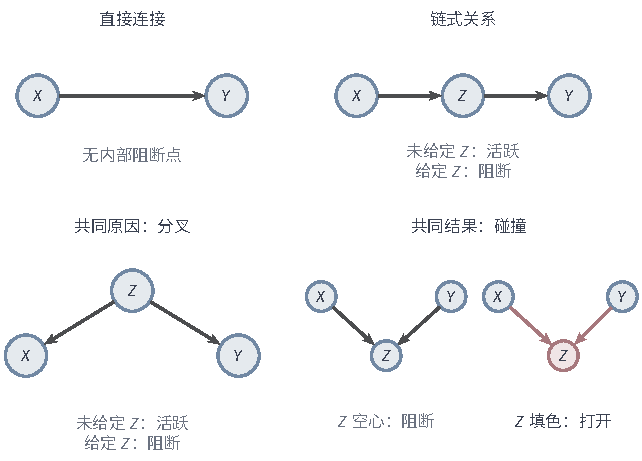
\includegraphics[width=108.793mm]{figures/06-probabilistic-graphical-models/01-representation/tikz/pgm-directed-motifs/figure.pdf}
  \caption{四种局部关系及观测中间节点后的路径变化。链和分叉在同一小图中对照两种状态；碰撞关系分为两列，空心$Z$表示未观测的阻断点，红色填充$Z$表示给定后打开的位置。活跃路径允许两端存在依赖，具体参数决定依赖是否出现。在大图中，观测碰撞点的后代也会打开该位置；直接连接没有内部阻断点。}
  \label{fig:pgm-directed-motifs}
\end{figure}

在直接连接$X\to Y$中，$X$进入$Y$的局部分布，路径中没有可用于阻断的中间节点。具体条件表若满足$p(y\mid x)=p(y)$，这个输入仍可能不改变分布，即该参数下$X\perp Y$。第~\ref{sec:pgm-directed-sound-complete}节将用数值例子说明结构允许的依赖与单个分布实际具有的依赖之间的区别。

链式关系$X\to Z\to Y$通过$Z$连接两端。采用顺序$X,Z,Y$，有序假设给出$Y\perp X\mid Z$，对应乘积$p(x,z,y)=p(x)p(z\mid x)p(y\mid z)$，一般等价证明见第~\ref{sec:pgm-representations-directed-proofs}节。给定一个满足$p(z)>0$的中间状态，条件联合分布为
\[
  p(x,y\mid z)=p(x\mid z)p(y\mid z).
\]
消去$Z$时，各个$z$下的条件分布混合在一起，两端通常仍有关联。将链反向画成$X\leftarrow Z\leftarrow Y$，给定中间节点后的独立关系相同。因此，路径判断考察内部节点的箭头形状，而非从某一端是否能沿箭头走到另一端。

分叉$X\leftarrow Z\to Y$以同一节点作为两端的条件，常用“共同原因”辨认其形状。给定$Z$时，图保证$X\perp Y\mid Z$；消去$Z$后，混合分布则可能相关。设$Z$等概率取$0$或$1$，给定$Z$后$X,Y$独立，并且两者取$1$的概率在$Z=1$时均为$0.9$，在$Z=0$时均为$0.1$。此时$p(X=1)=p(Y=1)=0.5$，而$p(X=1,Y=1)=(0.9^2+0.1^2)/2=0.41\ne0.25$。这个差值来自不同$Z$状态的混合，与每个固定$Z$下的条件独立相容。

碰撞结构$X\to Z\leftarrow Y$将两条箭头的终点放在同一个中间节点，也称“共同结果”结构。两个根节点独立，联合分解为$p(x)p(y)p(z\mid x,y)$，对$z$求和后得到$p(x,y)=p(x)p(y)$。给定$z$时，局部因子$p(z\mid x,y)$参与条件概率，可能使两端产生依赖。设$X,Y$是独立公平二值变量，$Z=1$当且仅当至少一个输入为$1$；给定$Z=1$时，$p(X=1\mid Z=1)=2/3$，再给定$Y=1$时则降为$1/2$。在这个参数设定中，确认$Y$已能解释共同结果，就降低了$X$取$1$的条件概率。这称为\term{解释消除}（explaining away），即观测共同结果后，不同解释之间产生竞争。具体依赖的方向和强弱仍由条件概率决定。

观测碰撞点的后代也可能提供关于碰撞点的信息，因此路径判据将这个位置视为打开。例如，在$X\to Z\leftarrow Y$后接$Z\to D$，若$D=Z$，观测$D$便等价于观测$Z$；若$D$是带噪声的测量，则传递的信息量取决于噪声水平。碰撞点及全部后代均未给定时，该位置才由图保证阻断。这里的“共同原因”和“共同结果”描述箭头形状，其因果解释需要另行建立。

\begin{figure}[htbp]
  \centering
  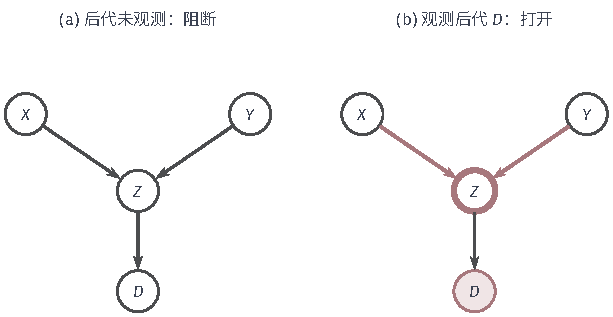
\includegraphics[width=103.720mm]{figures/06-probabilistic-graphical-models/01-representation/tikz/pgm-directed-collider-descendant/figure.pdf}
  \caption{后代观测对碰撞位置的作用。左图中$Z$及其后代均未给定，路径$X\to Z\leftarrow Y$被阻断；右图将后代$D$填色为观测，空心双圈$Z$标出已打开的碰撞位置，红色路径满足$Z\in\operatorname{an}^{+}(S)$。图上打开的路径允许依赖出现，依赖强度由分布决定。}
  \label{fig:pgm-directed-collider-descendant}
\end{figure}

\subsection{d-分离的定义}
\label{sec:pgm-directed-d-separation}

两组节点在给定条件后仍可能通过多条路径联系，因而分离查询需要汇总全部路径的判断。路径上的非碰撞点被给定时阻断路径，碰撞点自身或后代被给定时则打开该位置。对两两不交的$A,B,S\subseteq V$，若$A,B$之间不存在活跃路径，就记$A\perp_{\mathcal G}B\mid S$。这个记号先描述图上的分离，随后将说明它与概率独立的关系。为表达碰撞点的观测条件，后文用$\operatorname{an}^{+}(T)$表示包含$T$自身的祖先闭包。

设备路径中的$A$是碰撞点，$H$是非碰撞点，图~\ref{fig:pgm-directed-active-path}对照了给定它们后的变化。只给定$A$时路径活跃，再给定$H$时路径在$H$处阻断。整条路径活跃需要每个内部位置都满足条件，因此一个位置的打开无法消除另一位置的阻断。

\begin{figure}[htbp]
  \centering
  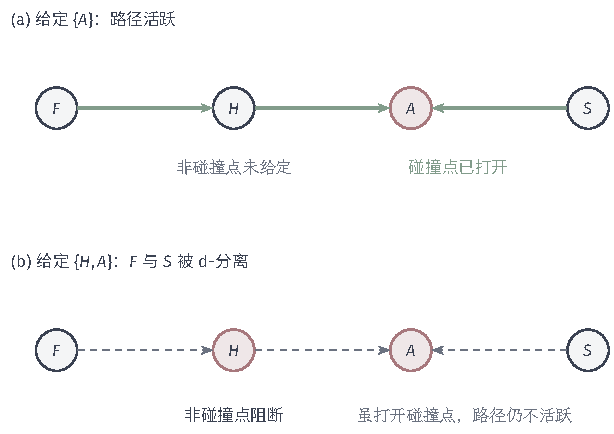
\includegraphics[width=103.904mm]{figures/06-probabilistic-graphical-models/01-representation/tikz/pgm-directed-active-path/figure.pdf}
  \caption{设备路径的活跃状态与d-分离。上图给定碰撞点$A$后，$F\to H\to A\leftarrow S$活跃；下图再给定非碰撞点$H$后，唯一的连接路径被阻断，得到$F\perp_{\mathcal{G}}S\mid(H,A)$。红色节点为给定变量，绿色实线为活跃路径，灰色虚线为阻断路径。}
  \label{fig:pgm-directed-active-path}
\end{figure}

图上的$A\perp_{\mathcal G}B\mid S$与分布中的$\bm{X}_A\perp\bm{X}_B\mid\bm{X}_S$分别描述路径和概率关系。\term{全局Markov性质}（global Markov property）把两者接起来：对每个两两不交的查询$(A,B,S)$，图中的d-分离蕴含相应的分布独立。第~\ref{sec:pgm-directed-sound-complete}节将说明相容分布为何满足这个蕴含。

\begin{lemma}[全局Markov性质蕴含局部Markov性质]
  \label{lem:pgm-representations-global-to-local}
  设$\mathcal{G}=(V,E)$为有限有向无环图，$p$为节点随机变量$\bm{X}=(X_i)_{i\in V}$的联合分布。若$p$满足$\mathcal{G}$的全局Markov性质，则$p$也满足该图的局部Markov性质，并进一步满足任一固定拓扑序下的有序Markov性质。
\end{lemma}

\begin{proof}[引理~\ref{lem:pgm-representations-global-to-local}的证明]
固定节点$i$，逐一考察它到非父、非后代节点的路径。路径若在$i$处经过一条入边，邻接的父节点就是内部非碰撞点，给定$\operatorname{pa}(i)$即可在此阻断。路径若先沿$i$的出边前进，则到达非后代之前必须改变沿箭头前进的方向；第一次转折产生一个碰撞点，并且该点是$i$的后代。这个碰撞点及其后代均在父集之外，否则有向路径与入边会构成环，因而给定父集后该碰撞点保持阻断。两类路径都被阻断，得到
\[
  i\perp_{\mathcal G}
  \operatorname{nd}(i)\setminus\operatorname{pa}(i)
  \mid\operatorname{pa}(i).
\]
将该图分离代入全局Markov性质，便得到局部Markov性质。合法拓扑序的前驱包含于非后代集合，从局部独立陈述中边缘化其他非后代，又得到该拓扑序下的有序Markov性质。
\end{proof}

在设备图中，$F,S$只有$F\to H\to A\leftarrow S$这一条连接路径。无观测时，碰撞点$A$阻断它，得到$F\perp S$；给定报警$A$后，碰撞位置打开而$H$保持未观测，路径转为活跃；再给定$H$后又得到$F\perp S\mid(H,A)$。如果增加$A\to D$，观测$D$同样会打开$A$，因为它提供了碰撞点后代的证据。

条件集合$S$记录被给定的变量，而具体取值另行指定。d-分离所对应的条件独立对条件变量分布几乎处处成立，涵盖整项条件关系。某些参数还可能只在特定条件取值下产生独立，这类上下文性质来自具体分布，须与图上的分离查询分别处理。

\subsection{d-分离的可靠性与特定场景下的完备性}
\label{sec:pgm-directed-sound-complete}

同一张图可以配上不同的条件概率表，路径判据因而需要在分布类上解释。分离查询应对所有相容分布成立，而未分离查询需要考察是否存在实际依赖的相容分布。记$\mathcal{M}(\mathcal{G})$为定义~\ref{def:pgm-directed-ordered}所给模型的分布类；第~\ref{sec:pgm-directed-factorization}节将说明它与按$\mathcal{G}$分解的分布类等价，证明见第~\ref{sec:pgm-representations-directed-proofs}节。

\begin{theorem}[d-分离的可靠性]
  \label{thm:pgm-directed-soundness}
  设$\mathcal{G}=(V,E)$为有限有向无环图，$A,B,S\subseteq V$两两不交且$A,B$非空。对每个$p\in\mathcal{M}(\mathcal{G})$，
  \begin{equation}
    A\perp_{\mathcal{G}}B\mid S
    \quad\Longrightarrow\quad
    \bm{X}_A\perp_p\bm{X}_B\mid\bm{X}_S.
    \label{eq:pgm-directed-soundness}
  \end{equation}
\end{theorem}

\begin{example}[未分离但独立的固定分布]
  \label{ex:pgm-directed-unseparated-independent}
  在只有一条边$X\to Y$的图中，令$X,Y\in\{0,1\}$，并设$p(X=0)=p(X=1)=1/2$。对每个$x\in\{0,1\}$，都取$p(Y=1\mid X=x)=1/3$和$p(Y=0\mid X=x)=2/3$。图上两个节点直接相邻，空集无法将它们d-分离；条件表的两行却相同，边缘化$X$得到$p(Y=1)=1/3$和$p(Y=0)=2/3$。由此对所有$x,y\in\{0,1\}$有
  \[
    p(X=x,Y=y)
    =
    p(X=x)p(Y=y)
    =
    \begin{cases}
      1/6,&y=1,\\
      1/3,&y=0.
    \end{cases}
  \]
  这个乘积等式给出该固定分布中的$X\perp Y$，说明相邻节点在某些参数下也能独立。
\end{example}

示例~\ref{ex:pgm-directed-unseparated-independent}区分了已选定的分布与可选的分布类。该分布中的依赖可以消失，而在充分丰富的分布类中，每项未分离查询仍有至少一个相容分布表现出依赖。后一种存在性结论称为\term{模型类完备性}，以下分别在严格正有限离散模型类与非退化线性高斯模型类中陈述。

\term{严格正有限离散模型}中，每个变量有有限个状态，每个完整配置的联合概率均大于$0$。固定状态空间$\mathcal{X}_i$并要求$|\mathcal{X}_i|\geq2$，将其中严格为正且按$\mathcal{G}$分解的质量函数记为$\mathcal{M}_{\mathrm{disc}}^{+}(\mathcal{G})$。\term{非退化线性高斯模型}则以父节点的线性函数加独立高斯噪声表示当前节点；正噪声方差保证联合分布具有完整维度。将所有由下式生成的分布记为$\mathcal{M}_{\mathrm{LG}}(\mathcal{G})$：
\[
  X_i=a_i+\sum_{j\in\operatorname{pa}(i)}b_{i,j}X_j+\varepsilon_i
\]
其中边系数$b_{i,j}$可取任意实数，噪声$\varepsilon_i$相互独立，满足$\varepsilon_i\sim\mathcal{N}(0,\sigma_i^2)$及$\sigma_i^2>0$。

\begin{theorem}[d-分离在特定模型类中的完备性]
  \label{thm:pgm-directed-completeness}
  设$\mathcal{G}=(V,E)$为有限有向无环图，$A,B,S\subseteq V$两两不交且$A,B$非空。若
  \[
    A\not\perp_{\mathcal{G}}B\mid S,
  \]
  则分别存在$p_{\mathrm{disc}}\in\mathcal{M}_{\mathrm{disc}}^{+}(\mathcal{G})$与$p_{\mathrm{LG}}\in\mathcal{M}_{\mathrm{LG}}(\mathcal{G})$，使
  \begin{equation}
    \bm{X}_A\not\perp_{p_{\mathrm{disc}}}\bm{X}_B\mid\bm{X}_S,
    \qquad
    \bm{X}_A\not\perp_{p_{\mathrm{LG}}}\bm{X}_B\mid\bm{X}_S.
    \label{eq:pgm-directed-completeness}
  \end{equation}
\end{theorem}

可靠性覆盖每个相容分布，模型类完备性则为每项未分离查询提供一个不独立的见证分布，不同查询还可以使用不同见证。两种结论采用不同量词，因此完备性与前面的固定分布反例相容。两个定理的证明见第~\ref{sec:pgm-representations-directed-proofs}节。

从观测到的条件独立反推图结构时，上例的相同行会造成歧义：独立可能来自缺边，也可能来自参数。

对于$p\in\mathcal{M}(\mathcal{G})$，模型的Markov性已经使图分离推出概率独立。忠实性进一步要求，每项分布独立都能由图分离解释（参见\BookDefinitionRef{def:causal-faithfulness}{卷2《数学准备：概率、因果与决策》第3章“因果响应”第3.6.1.1节“观测资料下的关系识别”}）。两个方向共同成立时，图与分布的独立关系集合相同。

确定性关系、强制参数共享和参数抵消都可能产生额外独立性。有向分解允许这些参数，而忠实性对分布施加进一步限制。结构学习在依据独立性删边时，需要说明所采用的忠实性假设及其适用依据。

\subsection{d-分离的检测}
\label{sec:pgm-directed-d-separation-testing}

路径判据可直接用于小图，但大图可能包含很多重复经过同一节点的路径。检测算法可以合并这些路径的到达状态，也可以将当前查询转为无向图的连通性检查。下面分别说明这两种计算方式如何利用结构。

\begingroup
% tufte-book禁用subsubsection；本节局部沿用其支持的第三级paragraph样式。
\let\subsubsection\paragraph

\subsubsection{Bayes--ball算法}
\label{sec:pgm-directed-bayes-ball}

设备图对$F,S$的查询只有一条连接路径，可以按内部节点的角色逐项检查，结果列于表~\ref{tab:pgm-directed-path-tests}。给定$H$使路径阻断，给定$A$则使碰撞位置打开，同时给定两者时仍由$H$阻断。观测增加后的变化由路径位置决定，而非条件集合大小决定。

\begin{table}[htbp]
  \centering
  \begin{tabularx}{\linewidth}{@{}lXX@{}}
    \toprule
    给定节点 & 路径上的检查 & 图的结论 \\
    \midrule
    $\varnothing$ & 碰撞点$A$未打开 & $F$与$S$分离 \\
    $\{H\}$ & 非碰撞点$H$阻断 & $F$与$S$分离 \\
    $\{A\}$ & $A$打开，$H$未阻断 & $F$与$S$连接 \\
    $\{H,A\}$ & $A$虽打开，$H$仍阻断 & $F$与$S$分离 \\
    \bottomrule
  \end{tabularx}
  \caption{设备路径$F\to H\to A\leftarrow S$在不同条件集合下的检查结果。“分离”给出图保证的独立性，“连接”表示结构允许依赖出现，实际依赖仍取决于参数。}
  \label{tab:pgm-directed-path-tests}
\end{table}
\FloatBarrier

为避免枚举可能呈指数增长的路径数，\term{Bayes--ball算法}（Bayes-ball algorithm）将搜索状态设为当前节点及到达方向，相同状态只处理一次。算法~\ref{alg:pgm-directed-bayes-ball}采用专门检测d-分离的版本，按照图结构传播状态；利用已知确定性关系作额外剪枝或计算后验属于其他任务。状态$(i,\uparrow)$表示从$i$的子节点一侧到达，$(i,\downarrow)$表示从父节点一侧到达。

\begin{algorithm}[Bayes--ball的d-分离检测]
  \label{alg:pgm-directed-bayes-ball}
  \begin{algorithmic}[1]
    \Require 有向图$\mathcal{G}=(V,E)$，两两不交的$A,B,S\subseteq V$，且$A,B$非空
    \Ensure “d-连接”或“d-分离”
    \State $R\gets\operatorname{an}^{+}(S)$
    \State 队列$Q\gets\{(a,\uparrow):a\in A\}$
    \State 已处理状态集$M\gets\varnothing$
    \While{$Q$非空}
      \State 从$Q$取出$(i,\delta)$
      \If{$(i,\delta)\in M$}
        \State 转到下一轮循环
      \EndIf
      \State $M\gets M\cup\{(i,\delta)\}$
      \If{$i\in B$}
        \State \Return d-连接
      \EndIf
      \If{$\delta=\uparrow$且$i\notin S$}
        \State 向$Q$加入$\{(j,\uparrow):j\in\operatorname{pa}(i)\}$
        \State 向$Q$加入$\{(j,\downarrow):j\in\operatorname{ch}(i)\}$
      \ElsIf{$\delta=\downarrow$}
        \If{$i\notin S$}
          \State 向$Q$加入$\{(j,\downarrow):j\in\operatorname{ch}(i)\}$
        \EndIf
        \If{$i\in R$}
          \State 向$Q$加入$\{(j,\uparrow):j\in\operatorname{pa}(i)\}$
        \EndIf
      \EndIf
    \EndWhile
    \State \Return d-分离
  \end{algorithmic}
\end{algorithm}

起点以子侧状态入队，使搜索能够沿入边和出边向外传播。从子侧到达$i$时，$i$在接续路径中是非碰撞点，满足$i\notin S$便可向父节点或子节点继续传播。从父侧到达$i$后，向子节点传播仍需$i\notin S$，向另一个父节点传播则在$i$处形成碰撞，需满足$i\in R$，即$i$自身或后代被观测。后两项判断独立执行，因此两种传播都可能发生；它们分别落实了路径定义中的非碰撞与碰撞条件。

在查询$F\perp S\mid A$中，$R=\{F,H,A,S\}$。搜索依次到达$F,H$，再从父侧到达$A$；因为$A$属于$R$，搜索转向其父节点$S$，发现一条活跃路径。将条件集合改为$\{H,A\}$后，观测节点$H$阻止向子节点$A$传播，搜索无法到达$S$。记录到达方向保留了这两类传播的区别，只有节点访问标记则会把不同搜索状态合并。

集合$R$通过从$S$逆向遍历祖先取得。随后每个节点至多处理两个到达状态，每条边由这些状态扫描常数次，因此时间和存储量均为$O(|V|+|E|)$\scite{pgm-directed-shachter1998}。

\subsubsection{祖先道德图检测}
\label{sec:pgm-directed-ancestral-moral-test}
\label{sec:pgm-directed-undirected-test}

同一个查询还可以通过\term{祖先道德图检测}转为连通性问题。保留$A\cup B\cup S$及其全部祖先，在这个子图中将共同子节点的父节点两两相连，再去掉箭头方向；删除条件节点$S$后，检查$A$与$B$是否连通。选取祖先子图这一步使转换依赖当前查询，区别于单纯去掉原图的方向。第~\ref{sec:pgm-representations-ancestral-moralization}节将正式定义该转换，证明它与d-分离等价，并分析代价。祖先道德图检测与Bayes--ball均输出结构分离结果，后验数值仍需概率运算。

\endgroup

\section{有向图中的因子分解}
\label{sec:pgm-directed-factorization}

\subsection{因子分解的定义}
\label{sec:pgm-directed-factor-definition}

设备模型的独立性假设确定了每个节点要保留的父节点条件，存储联合概率时则需要把这些局部分布组合起来。\term{有向因子分解}（directed factorization）将每个节点给定父节点的条件分布相乘。每一项都按当前节点归一化，使其在固定父配置下成为合法的条件分布。

组合局部函数还需要一个统一的联合积分空间。下文采用$\sigma$有限基准测度，即状态空间可由可数个有限测度的集合覆盖；有限或可数状态的计数测度以及实数轴上的Lebesgue测度都符合这一条件。单坐标的可测事件由$\mathcal A_i$记录，它们的笛卡尔积生成乘积$\sigma$代数$\bigotimes_i\mathcal A_i$，作为联合可测事件集合。分解式中的“$\mu$几乎处处”针对乘积基准测度的零测集，改变这些位置的密度不会改变积分所得概率；前面的条件独立等式则以条件变量的边缘分布为参照，两处采用的测度不同。

\begin{definition}[按有向图分解]
  \label{def:pgm-directed-factorization}
  给定有限有向图$\mathcal{G}=(V,E)$，其中$V=\{1,\ldots,d\}$。节点$i$取值于可测空间$(\mathcal{X}_i,\mathcal{A}_i)$，其上指定$\sigma$有限基准测度$\mu_i$；记$(\mathcal{X},\mathcal{A})=(\prod_{i\in V}\mathcal{X}_i,\bigotimes_{i\in V}\mathcal{A}_i)$及$\mu=\bigotimes_{i\in V}\mu_i$。设联合分布$p$对$\mu$绝对连续，并仍用$p(\bm{x})$表示其可测密度。对每个节点$i$，选定局部条件质量函数或条件密度版本
  \[
    q_i:
    \mathcal{X}_i\times
    \prod_{j\in\operatorname{pa}(i)}\mathcal{X}_j
    \longrightarrow[0,\infty).
  \]
  要求$q_i$关于相应乘积$\sigma$代数可测，并对每个父节点配置$\bm{x}_{\operatorname{pa}(i)}$满足
  \[
    \int_{\mathcal{X}_i}
    q_i(x_i\mid\bm{x}_{\operatorname{pa}(i)})\,\mathrm{d}\mu_i(x_i)=1.
  \]
  若
  \begin{equation}
    p(\bm{x})=\prod_{i=1}^{d}
      q_i(x_i\mid\bm{x}_{\operatorname{pa}(i)})
      \qquad\text{$\mu$几乎处处},
    \label{eq:pgm-directed-factorization}
  \end{equation}
  就称$p$按有向图$\mathcal{G}$分解。父集为空时，对应因子$q_i(x_i)$是归一化的边缘质量函数或密度。有限离散变量情形取$\mathcal{A}_i=2^{\mathcal{X}_i}$和计数测度$\mu_i$，上述积分即求和，$p$与$q_i$均为概率质量函数，式~\eqref{eq:pgm-directed-factorization}对每个完整配置$\bm{x}$逐点成立；零质量父配置采用本章约定的归一化条件质量函数版本。连续变量情形中，$q_i$是相对于已指定$\mu_i$的条件密度版本，式~\eqref{eq:pgm-directed-factorization}相对于已定义的乘积测度$\mu$几乎处处成立；在零测集上改变密度版本不改变所表示的分布。
\end{definition}

上述定义判断给定的联合分布$p$是否具有所需分解。实际构造模型时，常常先指定各节点的局部条件函数，再将它们相乘，此时需要验证乘积已经归一化。下面的引理给出这项保证，并进一步说明：若保留的节点集合包含自身的全部祖先，消去其余节点后，边缘密度就是保留节点的局部函数乘积。状态空间、基准测度、可测性和局部归一化的条件在引理中一并列出。

\begin{lemma}[局部归一化与祖先边缘化]
  \label{lem:pgm-directed-normalization}
  设$\mathcal{G}=(V,E)$为有限有向无环图，$V=\{1,\ldots,d\}$。节点$i$取值于可测空间$(\mathcal{X}_i,\mathcal{A}_i)$，其上给定$\sigma$有限基准测度$\mu_i$；有限离散变量取计数测度。对每个节点$i$，设局部函数
  \[
    q_i:
    \mathcal{X}_i\times
    \prod_{j\in\operatorname{pa}(i)}\mathcal{X}_j
    \longrightarrow[0,\infty)
  \]
  关于相应乘积$\sigma$代数可测，并对每个父节点配置满足
  \[
    \int_{\mathcal{X}_i}
    q_i(x_i\mid\bm{x}_{\operatorname{pa}(i)})\,\mathrm{d}\mu_i(x_i)=1.
  \]
  相对于乘积测度$\mu=\bigotimes_{i\in V}\mu_i$定义
  \[
    q(\bm{x})=\prod_{i\in V}
    q_i(x_i\mid\bm{x}_{\operatorname{pa}(i)}).
  \]
  则$q$归一化，因而是某个联合分布$p$的密度。更一般地，若$W\subseteq V$包含其中每个节点的全部祖先，则$p$关于$\mu_W=\bigotimes_{i\in W}\mu_i$的边缘密度满足
  \begin{equation}
    p(\bm{x}_W)=
    \prod_{i\in W}q_i(x_i\mid\bm{x}_{\operatorname{pa}(i)}).
    \label{eq:pgm-directed-ancestral-marginal}
  \end{equation}
  该等式对$\mu_W$几乎处处成立；有限离散情形中则对每个$\bm{x}_W$逐点成立。
\end{lemma}

无环结构使归一化能够从末端节点逐项消元，引理~\ref{lem:pgm-directed-normalization}的完整证明见第~\ref{sec:pgm-representations-directed-proofs}节。有向环的反例说明这个条件的作用：在二值环$X\to Y\to X$上取$q_X(x\mid y)=\mathbf{1}\{x=y\}$、$q_Y(y\mid x)=\mathbf{1}\{y=x\}$，两个条件表各自归一化，乘积在$(0,0)$和$(1,1)$上却都为$1$，总和为$2$。环使末端消元无法进行，所以局部归一化在这里没有给出联合归一化。

设备图中的四个局部表对应如下联合分解：
\begin{equation}
  p(f,h,a,s)=p(f)p(s)p(h\mid f)p(a\mid h,s).
  \label{eq:pgm-directed-device-factor}
\end{equation}
用第~\ref{sec:pgm-directed-discrete}节列出的教学参数，可以逐项求出配置$F=1,H=1,A=1,S=0$的联合概率：
\begin{equation}
  \begin{aligned}
    &p(F=1,H=1,A=1,S=0)\\
    &\quad=p(F=1)p(S=0)p(H=1\mid F=1)
      p(A=1\mid H=1,S=0)\\
    &\quad=0.1\times0.95\times0.8\times0.9
      =0.0684.
  \end{aligned}
  \label{eq:pgm-directed-device-configuration}
\end{equation}
计算结果$0.0684$来自四个局部表项的乘积，因而完整联合表中的这一项可以在使用时求得。消去变量时也能利用分解，例如求$F,H$的边缘分布，可以先汇总报警状态，再汇总传感器状态：
\[
  \begin{aligned}
    p(f,h)
    &=p(f)p(h\mid f)
      \sum_s p(s)\sum_a p(a\mid h,s)\\
    &=p(f)p(h\mid f).
  \end{aligned}
\]
内层报警概率的和为$1$，随后传感器概率的和也为$1$，因此只剩$F,H$的两个因子。有限求和的顺序可以交换，结果保持相同，中间函数的作用域与大小却可能改变。第~\ref{chap:pgm-elimination}章将据此分析消元顺序的计算代价。

\subsection{从因子分解到条件独立性}
\label{sec:pgm-directed-factor-to-ci}

在完整联合乘积中，$x_i$既出现在节点$i$自己的因子，也出现在子节点的因子中。要得到节点$i$给定非后代的条件分布，需要先边缘化后代，利用祖先边缘分解消去这些子节点因子。这样才可从剩余局部项读出所需独立性。

\begin{theorem}[分解蕴含局部与有序Markov性质]
  \label{thm:pgm-directed-factor-local}
  设$\mathcal{G}=(V,E)$为有限有向无环图，$p$为节点随机变量$\bm{X}=(X_i)_{i\in V}$的联合分布。若$p$按$\mathcal{G}$分解，则$p$满足该图的局部Markov性质，并满足该图任一固定拓扑序下的有序Markov性质。
\end{theorem}

定理~\ref{thm:pgm-directed-factor-local}将因子分解连接到局部和有序Markov性质，定理~\ref{thm:pgm-directed-soundness}的可靠性结论再将它连接到全局Markov性质。相应证明集中在第~\ref{sec:pgm-representations-directed-proofs}节。

\subsection{从条件独立性到因子分解}
\label{sec:pgm-directed-ci-to-factor}

反向构造从定义中的固定拓扑序开始。链式法则先为每个节点保留全部前驱条件，有序Markov假设再将其缩为父节点条件，从而得到所需乘积。

\begin{theorem}[有序假设导出有向分解]
  \label{thm:pgm-directed-ordered-factor}
  设$\mathcal{G}=(V,E)$为有限有向无环图，$p$为节点随机变量$\bm{X}=(X_i)_{i\in V}$的联合分布，并采用定义~\ref{def:pgm-directed-factorization}中的有限离散质量函数或连续密度设定。若$p$满足$\mathcal{G}$的某一个固定拓扑序下的有序Markov假设，则$p$按$\mathcal{G}$分解。
\end{theorem}

定理~\ref{thm:pgm-directed-factor-local}和定理~\ref{thm:pgm-directed-ordered-factor}给出有序性质与分解之间的两个方向，局部性质又蕴含有序性质。加上d-分离可靠性及全局到局部的蕴含，四种表述连成如下等价关系：
\begin{equation}
  \begin{aligned}
    \text{固定拓扑序的有序性质}
      &\Longleftrightarrow \text{按有向图分解}\\
      &\Longleftrightarrow \text{局部Markov性质}\\
      &\Longleftrightarrow \text{全局Markov性质}.
  \end{aligned}
  \label{eq:pgm-directed-equivalence}
\end{equation}
这个等价关系说明，一个拓扑序下的有序假设已经确定模型类：先由该序得到分解，再由分解得到任一合法拓扑序下的有序性质。上述有向结论允许零概率配置，与后文无向分解定理的严格正性要求有所区别。全局到局部的方向已由引理~\ref{lem:pgm-representations-global-to-local}证明，其余方向见第~\ref{sec:pgm-representations-directed-proofs}节。

式~\eqref{eq:pgm-directed-equivalence}检验一个给定分布的模型归属。定理~\ref{thm:pgm-directed-completeness}则处理另一种量词：对每个未分离查询，在指定模型类中构造至少一个不独立的见证分布。这项构造的证明也见第~\ref{sec:pgm-representations-directed-proofs}节。

\section{局部参数化}
\label{sec:pgm-directed-local-parameterization}

设备诊断的结构已确定报警使用$H,S$作条件，接下来还要给出每种条件下的报警概率。局部参数化负责记录这些数值，并支持估计和采样。本节分别讨论离散表与连续条件分布，它们提供不同的局部函数形式，共同遵循前面的有向分解。

\subsection{离散变量}
\label{sec:pgm-directed-discrete}

对于离散节点，父配置固定后，只需记录各个子状态的概率。若$X_i$有$r_i$个状态、父节点有$c_i=\prod_{j\in\operatorname{pa}(i)}r_j$种配置，\term{条件概率表}（conditional probability table, CPT）为每个父配置设置一个长度$r_i$的向量。各行非负且和为$1$，每行有$r_i-1$个自由参数，所以无额外约束的表共有$c_i(r_i-1)$个自由参数。对所有节点求和，得到网络的参数自由度：
\begin{equation}
  m=\sum_{i=1}^{d}(r_i-1)
       \prod_{j\in\operatorname{pa}(i)}r_j.
  \label{eq:pgm-directed-cpt-size}
\end{equation}
若每个变量最多有$r$个状态、每个节点最多有$k$个父节点，完整条件表的存储空间为$O(dr^{k+1})$。因此，父集大小决定一张局部表包含多少行，是控制离散表示规模的关键条件。

设备模型中的二值根节点各需一个参数，$H$的两个父配置和$A$的四个父配置分别需要两个、四个参数，总计$1+1+2+4=8$个。相同四变量的无约束联合表则需要$2^4-1=15$个参数。以下教学设定给出根节点与过热节点的局部数值：
\[
  \begin{aligned}
    p(F=1)&=0.1,& p(S=1)&=0.05,\\
    p(H=1\mid F=1)&=0.8,&
    p(H=1\mid F=0)&=0.1.
  \end{aligned}
\]
报警节点的四行列在表~\ref{tab:pgm-directed-alarm-cpt}中，每行取$0$的概率为取$1$概率的余数。

\begin{table}[htbp]
  \centering
  \begin{tabular}{@{}ccrr@{}}
    \toprule
    $h$ & $s$ & $p(A=1\mid h,s)$ & $p(A=0\mid h,s)$ \\
    \midrule
    $0$ & $0$ & $0.01$ & $0.99$ \\
    $1$ & $0$ & $0.90$ & $0.10$ \\
    $0$ & $1$ & $0.70$ & $0.30$ \\
    $1$ & $1$ & $0.99$ & $0.01$ \\
    \bottomrule
  \end{tabular}
  \caption{教学模型的报警条件概率表。每个固定$(h,s)$对应一行二值概率分布，两项之和为$1$；数值为人工设定。}
  \label{tab:pgm-directed-alarm-cpt}
\end{table}

用这些局部数值，可以计算章首所问的观测变化。先消去故障和传感器状态，得到过热与报警的概率：
\[
  \begin{aligned}
    p(H=1)&=0.1\times0.8+0.9\times0.1=0.17,\\
    p(A=1\mid H=1)&=0.95\times0.9+0.05\times0.99=0.9045,\\
    p(A=1\mid H=0)&=0.95\times0.01+0.05\times0.7=0.0445,\\
    p(A=1)&=0.17\times0.9045+0.83\times0.0445=0.1907.
  \end{aligned}
\]
报警后过热概率为$0.153765/0.1907\approx0.8063$。再给定传感器失灵，另一种解释进入条件，过热后验变为
\[
  p(H=1\mid A=1,S=1)
    =\frac{0.17\times0.99}
      {0.17\times0.99+0.83\times0.7}
    \approx0.2246.
\]
将仍未知的过热状态边缘化，同样可以比较故障在两组证据下的后验：
\[
  \begin{aligned}
    p(F=1\mid A=1)&=\frac{0.07325}{0.1907}\approx0.3841,\\
    p(F=1\mid A=1,S=1)&=\frac{0.0932}{0.7493}\approx0.1244.
  \end{aligned}
\]
在这组参数中，传感器失灵解释了一部分报警，使故障后验从约$0.3841$降到约$0.1244$。这是解释消除的一个具体数值结果，路径判据则说明给定报警为何允许两种解释发生关联。

完整观测数据还能直接估计这些表。设有$n$个独立同分布样本$\{\bm{x}_{\ell}\}_{\ell=1}^{n}$，所有节点均已观测，图固定且局部表参数没有共享约束。将父配置为$a$且$X_i=k$的样本数记为$N_{i,a,k}$，行计数记为$N_{i,a}=\sum_kN_{i,a,k}$，该项条件概率记为$\theta_{i,a,k}$。对数似然于是按节点和父配置分开，逐行最大化给出
\[
  \begin{aligned}
    \ell(\bm{\theta})
       &=\sum_i\sum_a\sum_kN_{i,a,k}\log\theta_{i,a,k},\\
    \widehat{\theta}_{i,a,k}&=\frac{N_{i,a,k}}{N_{i,a}}.
  \end{aligned}
\]
每行概率和为$1$的约束下，计数比例给出$N_{i,a}>0$时的极大值。$N_{i,a}=0$的行没有样本支持，数据无法确定该行的参数。加入正伪计数$\alpha_{i,a,k}$，可得到平滑估计$(N_{i,a,k}+\alpha_{i,a,k})/(N_{i,a}+\sum_k\alpha_{i,a,k})$，在Dirichlet先验下它是后验均值。缺失、潜变量与共享参数会改变这种逐行求解方式，第~\ref{chap:pgm-parameter-learning}章将继续讨论。

完整表之外，还可以利用已知局部规律减少参数。\term{参数共享}（parameter sharing）使不同父配置或不同节点复用参数，以较少自由度表示对称性，同时将模型限定在满足这些共享关系的分布中。\term{确定性节点}（deterministic node）由父节点唯一决定，其离散条件分布为$p(x_i\mid\bm{x}_{\operatorname{pa}(i)})=\mathbf{1}\{x_i=g_i(\bm{x}_{\operatorname{pa}(i)})\}$。这种规则允许部分配置具有零概率，有向分解的可靠性仍成立，具体分布也可能出现额外独立。

若父节点的作用只在某些条件取值下出现，可按部分父状态选择较小的表或决策树，这称为\term{上下文特定参数化}（context-specific parameterization）。另设一个报警模型，在传感器失灵时令$p(A=1\mid H=h,S=1)=0.8$对所有$h$相同，在$S=0$时仍保留对$H$的依赖。此时$A\perp H\mid S=1$只描述这一条件取值，完整的$A\perp H\mid S$并不成立，$H\to A$仍需保留。相同行、确定性规则或树状函数可以减少存储；推断若要利用这一节省，还需在运算中保持相应局部结构。

数值化后，完整配置的概率通过查表与乘积取得，条件查询则通常还要汇总未观测状态。朴素枚举的规模随未知变量数指数增长，结构化消元的开销又取决于中间作用域。因此，前面线性时间的d-分离检测描述的是图上查询，其复杂度与后验概率计算分别分析。

\subsection{连续变量}
\label{sec:pgm-directed-continuous}

温度等连续测量具有无限多个取值，需要用函数表示条件密度。一种常用选择是\term{线性高斯条件分布}（linear Gaussian conditional distribution），让父节点的线性函数给出条件均值，再用高斯噪声表示剩余变化。各节点的局部密度写为
\begin{equation}
  \begin{aligned}
    p(x_i\mid\bm{x}_{\operatorname{pa}(i)})
      &=\mathcal N\left(
        x_i;\,a_i+\sum_{j\in\operatorname{pa}(i)}b_{i,j}x_j,\,
        \sigma_i^2\right),\\
    \sigma_i^2&>0.
  \end{aligned}
  \label{eq:pgm-directed-linear-gaussian}
\end{equation}
截距$a_i$与系数$b_{i,j}$决定条件均值，方差$\sigma_i^2$决定固定父取值后的噪声大小。等价的生成方程采用相互独立的$\varepsilon_i\sim\mathcal N(0,\sigma_i^2)$。独立噪声使各局部分布按既定父集组合；若改用相关噪声，就需重新处理由噪声引入的节点间依赖。

为求整个系统的均值和协方差，将方程联立为$\bm X=\bm a+\bm B\bm X+\bm\varepsilon$，并记噪声协方差为$\bm D=\operatorname{diag}(\sigma_1^2,\ldots,\sigma_d^2)$。解这个线性系统得到
\[
  \begin{aligned}
    \bm{\mu}&=(\bm I-\bm B)^{-1}\bm a,\\
    \bm{\Sigma}&=(\bm I-\bm B)^{-1}
      \bm D\bigl((\bm I-\bm B)^{-1}\bigr)^{\top}.
  \end{aligned}
\]
按拓扑序排列后，$\bm B$严格下三角，因而$\bm I-\bm B$可逆；正噪声方差又使$\bm\Sigma$正定。这些局部高斯条件分布由此组成非退化联合高斯分布，归一化已经由有向乘积保证。每个节点包含$|\operatorname{pa}(i)|$个回归系数、一个截距和一个方差，共$|\operatorname{pa}(i)|+2$个参数，全图合计$|E|+2d$。

考虑一个三节点例子：$X_1\sim\mathcal N(0,1)$，$X_2=2X_1+\varepsilon_2$，$X_3=-X_2+\varepsilon_3$，其中$\varepsilon_2,\varepsilon_3$为独立标准高斯噪声，并与$X_1$独立。由链$1\to2\to3$计算得协方差矩阵
\[
  \bm\Sigma=
  \begin{pmatrix}
    1&2&-2\\
    2&5&-5\\
    -2&-5&6
  \end{pmatrix}.
\]
矩阵给出两端的边缘协方差$-2$，给定$X_2$后的条件协方差则为$-2-2(1/5)(-5)=0$。在联合高斯分布中，零条件协方差对应条件独立，与链的d-分离一致。这里的高斯条件至关重要，一般非高斯分布中的独立性还需要考察协方差之外的分布信息。

完整观测且图固定、参数互不共享时，可以逐节点将当前变量对父变量作带截距的最小二乘回归。各节点残差平方和为正的条件下，这给出式~\eqref{eq:pgm-directed-linear-gaussian}的最大似然估计，噪声方差由残差平方和除以$n$估计。设计矩阵满列秩保证系数唯一，秩不足则需加入约束或正则化。若残差完全为零并允许$\sigma_i^2$趋向零，似然无界增大，非退化模型内没有有限最大值。数据若呈非线性、异方差或多峰变化，还可选择相应的局部密度形式，同时保留有向分解语义。

设备运行工况可以是离散状态，温度则是连续测量，两者可用同一张图联合建模。\term{条件线性高斯模型}（conditional linear Gaussian model, CLG）按离散父配置分别设置线性高斯参数。对连续节点$i$，将离散父集记为$D_i$，连续父集记为$C_i$。固定$\bm X_{D_i}=\bm u$后，局部密度及均值写为
\[
  \begin{aligned}
    p(x_i\mid\bm u,\bm{x}_{C_i})
      &=\mathcal N\bigl(
        x_i;\,\mu_i(\bm u,\bm x_{C_i}),\sigma_{i,\bm u}^2\bigr),\\
    \mu_i(\bm u,\bm x_{C_i})
      &=a_{i,\bm u}+\bm b_{i,\bm u}^{\top}\bm{x}_{C_i}.
  \end{aligned}
\]
标准CLG的离散节点只采用离散父节点，连续节点则允许两类父节点。固定离散配置后的噪声方差为正，并且与连续父取值无关，因而给定全部离散变量后，连续部分构成联合高斯分布。消去离散变量后通常得到高斯混合。若以逻辑回归表示具有连续父节点的离散节点，所得分布仍是合法有向图模型，但属于更一般的模型类，其条件计算需要处理超出高斯封闭运算的部分。Koller与Friedman教材第5章介绍了相关模型范围\scite{pgm-koller2009}。

每个离散父配置需要一套系数、截距与方差，所以连续节点的自由参数数目为$\bigl(\prod_{j\in D_i}r_j\bigr)(|C_i|+2)$。离散父节点增多时，配置数仍可能指数增长。固定配置下的高斯条件化可用线性代数完成，汇总未知离散配置却仍可能涉及指数多个混合分量。

给定这些局部条件分布，还可以生成完整状态样本。\term{祖先采样}（ancestral sampling）按拓扑序遍历节点，在采样当前节点之前取得全部父节点的已生成取值，再从对应条件分布抽样。
\begin{algorithm}[有向图上的祖先采样]
  \label{alg:pgm-directed-ancestral-sampling}
  \begin{algorithmic}[1]
    \Require 一个有向图、归一化局部条件分布及拓扑序$1,\ldots,d$
    \Ensure 一个来自联合分布$p$的完整样本$\bm{x}$
    \For{$i=1,\ldots,d$}
      \State 读取已生成的父取值$\bm{x}_{\operatorname{pa}(i)}$
      \State 从$p(x_i\mid\bm{x}_{\operatorname{pa}(i)})$采样$x_i$
    \EndFor
    \State \Return $\bm{x}$
  \end{algorithmic}
\end{algorithm}
算法的采样顺序对应式~\eqref{eq:pgm-directed-factorization}，所以完整样本服从这些局部分布定义的联合分布。拓扑排序需要$O(d+|E|)$时间，随后还需逐节点选择局部分布并采样。表行选择和抽样均为常数时间时，遍历为线性开销；在线性高斯模型中，各节点条件均值计算合计为$O(d+|E|)$。更复杂局部分布的总成本则需加上各自的抽样代价。

例如，设备模型采用顺序$F,S,H,A$，并依次取得四个独立均匀数$0.08$、$0.40$、$0.60$和$0.85$。对二值节点，均匀数小于当前取$1$的概率时置$1$，否则置$0$，于是生成$F=1$、$S=0$、$H=1$、$A=1$。这个配置的联合概率为式~\eqref{eq:pgm-directed-device-configuration}中的$0.0684$。若要从给定$A=1$的后验采样，则需要让证据参与样本的选择或状态更新，例如拒绝完整样本中不满足证据者，或采用第~\ref{chap:pgm-sampling}章的条件采样方法。仅将$A$固定为$1$、其余节点仍按先验采样，会保留错误的父节点分布。这里的祖先顺序用于生成概率样本，其物理因果解释仍需额外假设。

\section{本章小结}
\label{sec:pgm-directed-summary}

报警后故障与传感器状态是否由图保证独立，取决于路径中的非碰撞点和碰撞点。给定链上的中间节点可以屏蔽两端，给定共同结果或其后代则可能建立解释之间的联系。d-分离将这些局部规则应用到全部连接路径，以条件集合和内部节点的角色回答结构上的独立性查询。

一个固定拓扑序下的有序Markov假设通过链式法则得到局部条件分布的乘积。祖先边缘化从乘积导出局部独立，d-分离可靠性导出全局独立，而全局到局部、局部到有序的蕴含又闭合了四种表述。这一等价关系使独立性假设与联合分解描述同一模型类，图还可据此指导归一化和采样。本章给出了全局到局部的图论证明，其余跨表示证明见第~\ref{sec:pgm-representations-directed-proofs}节。

条件表或连续局部密度给图补上参数，具体参数仍可能因抵消、确定性或上下文规律产生额外独立。可靠性为所有相容分布给出分离所保证的独立，模型类完备性为未分离查询提供存在依赖的见证，忠实性则进一步排除分布中的额外独立。数值参数化支持配置评价与生成样本，后验计算还须汇总未知状态，其成本由相应计算结构决定。

局部归一化与无环顺序共同保证了本章乘积的合法性。对适合用对称邻接描述的相互作用，联合分布将通过全局常数归一化。第~\ref{chap:pgm-undirected}章从无向分离出发，建立这种表示的因子分解及其成立条件。

\paragraph{扩展阅读}
Pearl的教材系统论述概率网络的独立性语义，Koller与Friedman的教材将这些关系接到表示、推断和学习算法上。两者对链、分叉、碰撞及后代观测的讨论，可补充本章从路径判断到模型类解释的讲解\scite{pgm-pearl1988,pgm-koller2009}。

\chapter{无向图模型}
\label{chap:pgm-undirected}

图像分割要为多个相邻像素同时分配标签。考虑一张二值化图片：每个区域要么属于前景，要么属于背景，孤立判断某一个区域往往不够可靠，还要借助它周围区域的信息。一个最朴素、也最常用的先验是：空间上相邻的像素更可能属于同一物体，因而更倾向于取相同标签。这种关系没有天然的先后或因果方向——并不是左侧像素“导致”右侧像素取某值，两个相邻区域只是互相约束。要把这种对称的“相邻相容”直接写进概率模型，有向边的父子条件分布就不再是最顺手的工具，于是需要一种不指定方向的图。

第~\ref{chap:pgm-directed}章的有向模型为每条边选定方向，并把联合分布组织成一组条件分布的乘积，每个节点的条件分布只依赖它的父节点。本章改用无向边：边只表示两个变量之间存在直接的局部相互作用，不再区分谁条件于谁。描述时也换成一套对称的语言——为“相邻变量取值协调”的配置赋予较高权重，再把所有局部权重相乘并做全局归一化，得到整个标签配置的概率。给定一部分区域的观测后，还可以进一步判断：被观测区域隔开的另外两组区域，是否还保留依赖。

这两件事正好对应无向图模型的两条主线，也是本章前半与后半的内容。其一是独立性语义：路径被观测节点阻断意味着什么，怎样由图上的邻接关系读出条件独立。本章会依次给出成对、局部和全局三种Markov性质，并比较它们在一般分布与严格正分布下的强弱关系。其二是概率表示：怎样把“局部相容”落实为团上的局部函数乘积，这个乘积与前述独立性之间能否互相推导。由独立性反推乘积分解时，零概率配置会限制可使用的局部组合；连续变量还涉及密度的积分与版本。因此，各个方向的推理都将连同相应的正性、测度和归一化条件一起说明，而不是把在一个方向上成立的结论直接套用到另一方向。

\section{无向图模型的定义}
\label{sec:pgm-undirected-definition}

用$X_1,\ldots,X_4$表示四个相邻区域的二值标签，并将它们按空间邻接连成环：$1$与$2$、$2$与$3$、$3$与$4$、$4$与$1$相邻。之所以选环而不是一条直链，是因为环上两个不相邻的节点之间仍有两条不同的连接路径（例如$1$与$3$既可经过$2$、也可经过$4$相连），这恰好能检验“要给定哪些节点才能真正把两侧隔开”，是后面讨论分离时最小而又不太平凡的例子。环上的每条边记录一对相邻区域之间的直接局部相互作用，边没有方向，只说明这两个区域的取值会彼此影响。后文采用这个人工模型计算条件概率，并通过改变配置的支持集，检查分离关系与严格正性条件的作用。

本章采用有限简单无向图$\mathcal G=(V,E)$，节点集为$V=\{1,\ldots,d\}$，并排除自环与重边。图的表示与邻接约定可参考\BookChapterRef{chap:graph-objects}{卷1《数学准备：计算、分析与几何》“图”部分的“图的对象与表示”章}。与$i$直接相连的节点组成邻居集合：
\[
  N(i)=\{j\in V:\{i,j\}\in E\}.
\]
每个节点$i$对应标量随机变量$X_i$，小写$x_i$表示其取值。将节点集合$A\subseteq V$中的变量组成向量，记为$\bm{X}_A$，其取值记为$\bm{x}_A$。节点编号描述图中的位置，状态描述变量的结果，例如$1\in V$指定节点，$x_1=0$指定该节点的一次取值。

从节点$i$沿现有边走到$j$，并使每个节点只出现一次，所得序列称为\term{路径}（path）。彼此有路径可达且无法继续扩大的节点集合称为\term{连通分量}（connected component）。若只保留节点集合$D$及其内部全部原有边，就得到\term{诱导子图}（induced subgraph）$\mathcal{G}[D]$。删除观测节点后检查剩余连通分量，将是无向分离检测的主要操作。

局部函数若涉及多个变量，需要先说明哪些变量组合由图允许放在同一个局部函数中。自然的要求是：只有两两之间都有直接相互作用的变量，才允许共用一个局部函数，否则就会在没有边的变量之间凭空引入直接依赖。任意两个不同节点都相邻的非空集合称为\term{团}（clique），单节点集合也自然属于团。一个团若加入任何其他节点都会破坏这一性质，就称为\term{极大团}（maximal clique）；这里的极大性针对包含关系，指它已经不能再扩大，并不表示其中的节点数在全图最多。图~\ref{fig:pgm-undirected-cliques}左侧的环有四个二节点极大团，三节点集合都缺少一条边；右侧的两个三角形分别给出极大团$\{1,2,3\}$与$\{3,4,5\}$。

\begin{figure}[htbp]
  \centering
  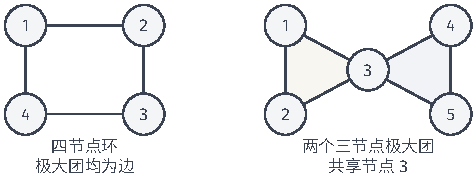
\includegraphics[width=80.652mm]{figures/06-probabilistic-graphical-models/01-representation/tikz/pgm-undirected-cliques/figure.pdf}
  \caption{无向图中的团与邻接。左图的四条边分别构成极大团，整个环因缺少对角边而不构成团；右图的两个三角形为极大团，共享节点$3$。无向线段表示邻接，节点编号对应随机变量下标。}
  \label{fig:pgm-undirected-cliques}
\end{figure}

观察一组节点后，两侧之间若已没有剩余路径，就用条件独立描述两侧的概率关系。采用这种语义的模型称为\term{无向图模型}（undirected graphical model），也称\term{Markov随机场}（Markov random field, MRF）或Markov网络。第~\ref{sec:pgm-undirected-global-independence}节将对任意节点集合正式陈述这项全局要求。

同一张无向图可以配上不同的局部函数，得到不同的分布。图只规定相容分布必须遵守的独立性，是对一整类分布的约束；数值参数则决定相邻变量实际具有多强的依赖。需要强调的是，图的保证只是“不强制相关”：如果某条边对应的相互作用强度取成零，两端变量仍可能独立，这种图没有要求的额外独立性完全可以出现。反过来，图中不存在的路径所对应的独立关系，却是相容分布都必须满足的。此外，无向边首先描述概率相互作用，并不说明干预某一端会如何改变另一端的分布；干预后的因果问题需要额外的因果建模语义，不能直接从无向边读出。这里采用的分离与Markov语义见无向图模型的标准表述\scite{pgm-lauritzen1996}。

\section{无向图的局部独立性}
\label{sec:pgm-undirected-local-independence}

在四节点环中，可以从两个不同粒度提出独立性问题。最直接的一种是盯住一条缺边：既然$1$与$3$之间没有边，那么在其余变量都已知的条件下，它们是否独立？这给出成对Markov性质。另一种是盯住一个节点：要预测$X_1$，需要知道哪些节点的取值，知道哪些之后其余节点就不再提供新信息？这给出局部Markov性质。两种问法涉及的独立侧和条件侧都不同，一个只处理一对节点，一个把一个节点与全部非邻居整体比较。它们看似相近，强弱却不完全相同，本节先分别建立这两种性质并讨论它们的关系，第~\ref{sec:pgm-undirected-global-independence}节再说明怎样由这些局部要求恢复任意集合之间的全局独立性。

\subsection{成对Markov性质}
\label{sec:pgm-undirected-pairwise}

两个非邻接节点$i,j$仍可能经其他节点相连。在环中$1$与$3$没有边，却同时经由$2$和$4$联系；若什么都不给定，两者的取值通常相关。成对Markov性质的想法是：把连接它们的所有中间节点全部给定，让每一条间接路径都被屏蔽，此时再要求这两个非邻接变量条件独立。条件侧取“其余全部节点”，正是为了不漏掉任何一条仍能传递信息的路径。

\begin{definition}[成对Markov性质]
  \label{def:pgm-undirected-pairwise}
  联合分布$p$相对于$\mathcal{G}$满足\term{成对Markov性质}（pairwise Markov property），是指对每一对不同且不相邻的节点$i,j$，都有
  \begin{equation}
    X_i\perp X_j\mid\bm{X}_{V\setminus\{i,j\}}.
    \label{eq:pgm-undirected-pairwise}
  \end{equation}
\end{definition}

四节点环中的非邻接对为$\{1,3\}$和$\{2,4\}$，对应的成对约束为
\[
  X_1\perp X_3\mid(X_2,X_4),
  \qquad
  X_2\perp X_4\mid(X_1,X_3).
\]
第一项同时以$X_2,X_4$为条件，这两个节点分别位于两条连接路径上。只给定$X_2$时，路径$1-4-3$仍然存在，结构尚未保证$X_1\perp X_3\mid X_2$。

这里需要区分离散与连续两种情形，因为它们“给定一个条件”的方式不同。对于离散变量，条件概率由概率的比值定义，只有在条件事件概率$p(\bm{x}_{V\setminus\{i,j\}})>0$时才有意义；二元条件独立就要求在这些正概率的条件配置下，条件联合概率等于两个条件边缘的乘积。若某个条件组合根本不会出现，对应的比值没有定义，自然也不能用同一比值去约束它。连续变量取特定值的概率通常为零，无法再用事件概率作比，因此改用条件密度或正则条件分布来表述，等式按条件变量的分布几乎处处成立；其严格依据与离散情形依赖正概率单点的论证并不相同。

成对性质便于按缺边列出约束，而集合查询还要同时处理多个变量。将一些已给定的变量移回未知侧会改变条件分布，因而从成对约束得到较大集合的独立性，需要相应的概率运算规则。后面的弱并与交性质将分别处理两种集合变化。

\subsection{局部Markov性质}
\label{sec:pgm-undirected-local}

现在换一种问法：固定一个节点$i$，想知道预测它时最少需要观测谁。从$i$出发到任何非邻居的路径，第一步都必须经过它的某个邻居$N(i)$；不经过邻居，就无法沿边走到图的其他部分。因此，一旦把全部邻居的值给定，$i$与所有非邻居之间的图上通道都被挡住。局部Markov性质把这一图上的屏蔽翻译成概率上的条件独立：给定邻居后，$X_i$与其余所有非邻居联合独立。

\begin{definition}[局部Markov性质]
  \label{def:pgm-undirected-local}
  联合分布$p$相对于$\mathcal{G}$满足\term{局部Markov性质}（local Markov property），是指对每个$i\in V$，都有
  \begin{equation}
    X_i\perp\bm{X}_{V\setminus(\{i\}\cup N(i))}
       \mid\bm{X}_{N(i)}.
    \label{eq:pgm-undirected-local}
  \end{equation}
\end{definition}

给定某个节点集合后，若$X_i$与集合以外的其他变量独立，形象地说这个集合像一层“毯子”把$X_i$与外部隔开，就称为$X_i$的\term{Markov毯}（Markov blanket）。满足局部Markov性质时，邻居集合$N(i)$就是图所保证的一层毯：知道邻居后，再知道任何更远的节点都不会改变对$X_i$的判断。图~\ref{fig:pgm-undirected-markov-blanket}以中心、邻居和远端节点三层展示这一结构：所有通向远端的路径都先经过邻居。

\begin{figure}[htbp]
  \centering
  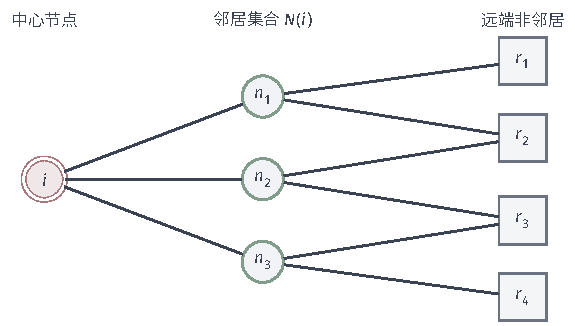
\includegraphics[width=97.402mm]{figures/06-probabilistic-graphical-models/01-representation/tikz/pgm-undirected-markov-blanket/figure.pdf}
  \caption{邻居集合构成的图上Markov毯。双边框圆为中心节点$i$，单边框圆为邻居$n_1,n_2,n_3$，方形为远端非邻居。实线均表示现存的无向边，中心到远端的每条路径先经过$N(i)$中的节点。}
  \label{fig:pgm-undirected-markov-blanket}
\end{figure}

在相应条件分布有定义的取值上，给定全部其他变量与只给定邻居得到相同的局部分布：
\begin{equation}
  p(x_i\mid\bm{x}_{V\setminus\{i\}})
  =p(x_i\mid\bm{x}_{N(i)}).
  \label{eq:pgm-undirected-blanket}
\end{equation}
该式把局部Markov性质落成一个可直接使用的结论：要计算某个节点在给定其余全部节点时的条件分布，只需查看它的邻居，远端节点的取值可以忽略。这正是后面许多局部计算（例如逐节点采样）只需邻居信息的根据。不过$N(i)$只是图在一般情况下保证的一层毯；对某个具体分布$p$，参数上的冗余可能允许更小的毯，例如某个邻居实际上从不改变局部分布，就可以把它省去。还要注意，即使图含有环，邻居仍然能屏蔽离开$i$的所有路径——因为任何这样的路径第一步必经过邻居，与后面是否绕成环无关，所以这项结构保证始终成立。

\begin{figure}[htbp]
  \centering
  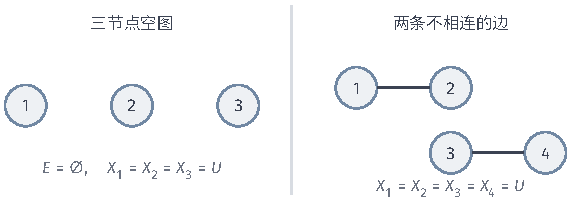
\includegraphics[width=96.686mm]{figures/06-probabilistic-graphical-models/01-representation/tikz/pgm-undirected-markov-counterexamples/figure.pdf}
  \caption{检验Markov性质逆向蕴含的两张图。各节点变量都等于同一个公平二值变量$U$，联合分布只有两个正概率配置。左侧空图满足成对性质而不满足局部性质；右侧两条不相连的边满足局部及成对性质而不满足全局性质。}
  \label{fig:pgm-undirected-markov-counterexamples}
\end{figure}

局部性质的结论强于成对性质：局部性质只给定邻居，却要求$X_i$与全部非邻居联合独立；成对性质给定其余全部节点，只要求其中一对独立。对一般分布，仅凭成对性质推不出局部性质，需要用退化分布说明；反过来，局部性质总能推出成对性质。

\begin{example}[成对性质不蕴含局部性质]
  \label{ex:pgm-undirected-pairwise-not-local}
  在图~\ref{fig:pgm-undirected-markov-counterexamples}左侧的三节点空图中，采用公平Bernoulli变量$U$，将三个节点都设为它的副本：
  \[
    X_1=X_2=X_3=U.
  \]
  空图的三对节点均不相邻，对应的全部成对约束是
  \[
    X_1\perp X_2\mid X_3,\qquad
    X_1\perp X_3\mid X_2,\qquad
    X_2\perp X_3\mid X_1.
  \]
  对第一项，在给定$X_3=u$的正概率事件下，两个未知变量也被确定为$u$。因此，对任意$u,a,b\in\{0,1\}$有
  \[
    \begin{aligned}
      p(X_1=a,X_2=b\mid X_3=u)
      &=\mathbf{1}\{a=u\}\mathbf{1}\{b=u\}\\
      &=p(X_1=a\mid X_3=u)p(X_2=b\mid X_3=u).
    \end{aligned}
  \]
  将$(X_1,X_2;X_3)$分别换为$(X_1,X_3;X_2)$和$(X_2,X_3;X_1)$，其余两项具有同样的指标函数乘积。三个成对约束由此全部成立。

  节点$1$的邻居集合$N(1)=\varnothing$，局部性质因而要求边缘独立$X_1\perp(X_2,X_3)$。比较全零状态的联合概率与边缘乘积，得到
  \[
    p\bigl(X_1=0,(X_2,X_3)=(0,0)\bigr)=\tfrac12
    \neq
    p(X_1=0)p\bigl((X_2,X_3)=(0,0)\bigr)=\tfrac14.
  \]
  两边分别为$1/2$和$1/4$，所以局部性质失败。分布只在$(0,0,0)$与$(1,1,1)$上为正，给定一个副本可以完全确定其他副本，而消去这个条件后，变量仍共同随$U$变化。这说明成对约束与无条件集合独立在当前支持集下有不同含义。
\end{example}

\begin{theorem}[局部Markov性质蕴含成对Markov性质]
  \label{thm:pgm-undirected-local-to-pairwise}
  设$\mathcal{G}=(V,E)$为有限简单无向图，$p$为节点随机变量$\bm{X}=(X_i)_{i\in V}$的任意联合分布。若$p$相对于$\mathcal{G}$满足局部Markov性质，则它满足成对Markov性质；该结论不要求$p$严格为正。
\end{theorem}

\begin{proof}
取一对任意不相邻节点$i,j$，并将$i$的非邻居记为$R=V\setminus(\{i\}\cup N(i))$，其中$j\in R$。由局部性质得到
\[
  X_i\perp\bm{X}_R\mid\bm{X}_{N(i)}.
\]
为了只保留$j$作为独立侧，需要把其余非邻居从独立侧移入条件集合。\term{弱并}（weak union）正是允许这种移动的条件独立运算规则：如果$X$在给定$W$后与$(Y,Z)$整体独立，那么再额外知道$Z$后，$X$仍与$Y$独立——本来就无关的信息，多知道一部分不会使其变得有关。写成式子即
\[
  X\perp(Y,Z)\mid W
  \quad\Longrightarrow\quad
  X\perp Y\mid(W,Z).
\]
前提使$p(x\mid y,z,w)=p(x\mid w)$，再按$p(y\mid z,w)$汇总$y$，得到$p(x\mid z,w)=p(x\mid w)$。两式右侧相同，所以给定$(Z,W)$后，再给定$Y$仍保持$X$的分布。这里使用相应条件分布有定义的配置，连续情形按条件变量分布几乎处处成立；这一转换允许联合分布取零值。

将$R$分为$\{j\}$与$R\setminus\{j\}$，把后一部分通过弱并移入条件，便有
\[
  X_i\perp X_j
  \mid\bigl(\bm{X}_{N(i)},\bm{X}_{R\setminus\{j\}}\bigr).
\]
条件侧合并了邻居与$j$之外的非邻居，恰好是$V\setminus\{i,j\}$。所得独立式就是这对节点的成对Markov约束，任意非邻接对都可采用同样的步骤。
\end{proof}

局部性质以邻居为条件，联合约束全部非邻居；成对性质以其他全部节点为条件，只约束其中一对。四节点环的每个节点恰有一个非邻居，所以该图中两种式子重合。链$1-2-3-4$则呈现差别：节点$1$的局部式是$X_1\perp(X_3,X_4)\mid X_2$，而相应两条成对式为$X_1\perp X_3\mid(X_2,X_4)$和$X_1\perp X_4\mid(X_2,X_3)$。要由后两条合并出前一条，相当于把$X_3,X_4$从条件侧一起移到独立侧；上面的弱并只能把变量从独立侧移到条件侧，方向恰好相反，无法完成这一合并。这需要下一节的交性质，而交性质只在严格正等条件下成立，这也解释了为什么两种性质在一般分布下并不等价。

\section{无向图的全局独立性}
\label{sec:pgm-undirected-global-independence}

成对和局部性质都只处理“一个或一对节点”层面的独立，而实际查询往往涉及两组区域。在图~\ref{fig:pgm-undirected-cliques}右侧，两个三角形区域分别为$\{1,2,3\}$与$\{3,4,5\}$，共享节点$3$。设想已知共享区域$3$的标签，想知道左侧区域$\{1,2\}$与右侧区域$\{4,5\}$是否还相互影响——这正是图像分割中“知道交界处后，左右两块能否分别推断”的问题。它的两侧都含多个变量，不能只靠单节点的局部式回答，需要考察连接两组节点的全部路径。

\subsection{全局Markov性质}
\label{sec:pgm-undirected-global}

左右两组节点被观测集合隔开时，所需结论是两组随机向量条件独立。\term{全局Markov性质}（global Markov property）把“路径阻断”这一图上事实统一翻译成概率约束：只要连接$A$与$B$的每一条路径都经过$S$中的某个节点，给定$\bm{X}_S$后两组变量就条件独立。它允许$A$、$B$是任意节点集合，$S$是任意能挡住全部路径的集合，因而前面的成对、局部性质都可以看作它在取特定集合时的特例。

\begin{definition}[全局Markov性质]
  \label{def:pgm-undirected-model}
  设$p$为$\bm{X}=(X_1,\ldots,X_d)^{\top}$的联合分布。若对任意两两不交的节点集合$A,B,S\subseteq V$，只要从任意$a\in A$到任意$b\in B$的每条路径都经过$S$中的节点，就有
  \begin{equation}
    \bm{X}_A\perp\bm{X}_B\mid\bm{X}_S,
    \label{eq:pgm-undirected-global}
  \end{equation}
  则称$p$相对于$\mathcal{G}$满足全局Markov性质，$(\mathcal{G},p)$构成一个无向图模型。
\end{definition}

定义从路径阻断推出分布独立，具体参数还可以给出图中未记录的额外独立性。在两个三角形共享节点$3$的例子中，从$\{1,2\}$到$\{4,5\}$的每条路径都经过$3$，因此得到
\[
  (X_1,X_2)\perp(X_4,X_5)\mid X_3.
\]
给定$X_3$后，联合条件分布分成左侧和右侧两个二元分布。每一侧内部仍可保留依赖，例如$X_1,X_2$同处一个三节点团，当前分离查询没有将它们分开。

查询集合与条件集合还可以只覆盖部分节点，即$A\cup B\cup S\neq V$。只查询$X_1,X_5$并给定$X_3$时，$X_2,X_4$留在未查询、未观测侧，同一路径判据仍给出$X_1\perp X_5\mid X_3$。证明全局性质因此还需边缘化这些剩余变量，处理三个集合未覆盖全部节点的情形。

\begin{theorem}[全局Markov性质蕴含局部与成对Markov性质]
  \label{thm:pgm-undirected-global-implications}
  设$\mathcal{G}=(V,E)$为有限简单无向图，$p$为节点随机变量$\bm{X}=(X_i)_{i\in V}$的任意联合分布。若$p$相对于$\mathcal{G}$满足全局Markov性质，则它同时满足局部与成对Markov性质。换言之，不附加严格正性时总有
  \begin{equation}
    \text{全局Markov}
    \ \Longrightarrow\ \text{局部Markov}
    \ \Longrightarrow\ \text{成对Markov}.
    \label{eq:pgm-undirected-implication}
  \end{equation}
\end{theorem}

\begin{proof}
固定$i\in V$，考察它到非邻居的路径。每条路径离开$i$后的首个节点都属于$N(i)$，所以$N(i)$分离$\{i\}$与$V\setminus(\{i\}\cup N(i))$。对这三个集合应用全局Markov性质，得到
\[
  X_i\perp\bm{X}_{V\setminus(\{i\}\cup N(i))}
  \mid\bm{X}_{N(i)},
\]
这正是节点$i$的局部约束。对全部节点重复该步骤，$p$便满足局部性质，再由定理~\ref{thm:pgm-undirected-local-to-pairwise}得到成对性质。
\end{proof}

上面的推导只用到“路径必经过邻居”这一图上事实和条件独立的基本运算，没有对概率取零作任何限制，所以“全局$\Rightarrow$局部$\Rightarrow$成对”对任意分布都成立。自然要追问反方向：能否从较弱的成对、局部性质重建出较强的全局性质？如果能，三种表述就只是同一约束的不同写法；如果不能，就需要弄清缺了什么条件。下面考察图~\ref{fig:pgm-undirected-markov-counterexamples}右侧的两个连通分量，用一个退化分布看到反方向确实可能失效：它满足各节点的局部约束，却在两个不相连的分量之间保留了共同随机性。

\begin{example}[局部、成对均不蕴含全局]
  \label{ex:pgm-undirected-local-not-global}
  将边集设为$E=\{\{1,2\},\{3,4\}\}$，四个变量仍取同一个公平二值变量的值：
  \[
    X_1=X_2=X_3=X_4=U,
    \qquad U\sim\operatorname{Bernoulli}(\tfrac12).
  \]
  两条边分别给每个节点提供一个邻居，局部性质要求
  \[
  \begin{aligned}
    X_1&\perp(X_3,X_4)\mid X_2,&
    X_2&\perp(X_3,X_4)\mid X_1,\\
    X_3&\perp(X_1,X_2)\mid X_4,&
    X_4&\perp(X_1,X_2)\mid X_3.
  \end{aligned}
  \]
  第一项给定$X_2=u$后，其他变量也随之确定。因此，对任意$u,a,r_3,r_4\in\{0,1\}$有
  \[
  \begin{aligned}
    &p(X_1=a,X_3=r_3,X_4=r_4\mid X_2=u)\\
    &\quad=\mathbf{1}\{a=u\}
            \mathbf{1}\{r_3=u,r_4=u\}\\
    &\quad=p(X_1=a\mid X_2=u)
            p(X_3=r_3,X_4=r_4\mid X_2=u).
  \end{aligned}
  \]
  将条件变量依次换为$X_1,X_4,X_3$，单节点端点依次换为$X_2,X_3,X_4$，便得到其余三项相同的指标函数分解。每一项都在正概率条件事件上成立，因此四项局部约束均被满足。

  不相邻的节点对为$\{1,3\}$、$\{1,4\}$、$\{2,3\}$与$\{2,4\}$，对应成对约束为
  \[
  \begin{gathered}
    X_1\perp X_3\mid(X_2,X_4),\qquad
    X_1\perp X_4\mid(X_2,X_3),\\
    X_2\perp X_3\mid(X_1,X_4),\qquad
    X_2\perp X_4\mid(X_1,X_3).
  \end{gathered}
  \]
  在任一缺边$\{i,j\}$的查询中，其余两个变量的正概率条件取值均为$(u,u)$。给定这样的取值后，
  \[
    p(X_i=a,X_j=b\mid\bm{X}_{V\setminus\{i,j\}}=(u,u))
    =\mathbf{1}\{a=u\}\mathbf{1}\{b=u\}.
  \]
  两个指标函数分别是条件边缘概率，故该式验证了四项成对独立。

  两个分量之间原本没有路径，全局性质要求$(X_1,X_2)\perp(X_3,X_4)$。然而它们共同随$U$变化，例如
  \[
    p(X_1=0,X_3=0)=\tfrac12
    \neq p(X_1=0)p(X_3=0)=\tfrac14.
  \]
  两个向量若独立，其分量$X_1,X_3$也应独立。上式的联合概率与边缘乘积不同，因此这个分布违背全局性质。
\end{example}

这两个反例能成立，关键都在于条件变量一旦给定，未知状态就被唯一确定，此时条件独立在一个退化为单点的条件分布上“平凡地”成立，它对其余取值组合没有任何约束力。逐变量的成对约束因此无法拼接成更大集合的独立。若要求完整乘积状态空间上的每一个配置都严格为正，任何条件组合就都真正可能发生，每一项条件独立都能在全部相关取值上使用，这就为合并这些约束提供了充分条件。

合并时需要一条与弱并方向相反的概率运算规则——交性质。设各坐标状态集有限且非空，并要求联合质量在完整乘积空间的每个配置上严格为正。对两两不交的索引集$A,B,C,D$，合并时使用的两个前提为
\[
  \bm{X}_A\perp\bm{X}_B\mid(\bm{X}_C,\bm{X}_D),
  \qquad
  \bm{X}_A\perp\bm{X}_D\mid(\bm{X}_C,\bm{X}_B).
\]
前一项表示给定$C,D$后，再知道$B$对$X_A$没有影响；后一项表示给定$C,B$后，再知道$D$对$X_A$也没有影响。交性质把两者合并为更强的结论：只给定$C$时，$X_A$与$(B,D)$整体都独立，即
\[
  \bm{X}_A\perp(\bm{X}_B,\bm{X}_D)\mid\bm{X}_C.
\]
与弱并相反，这条合并并不是无条件成立的——它要求$B$与$D$的每种组合都能在给定$C$时真正出现，否则“分别独立”的信息无法叠加；严格正性恰好排除了那种条件一给、其余状态就被锁死的退化情形，保证两组条件变量的每种组合都能作为条件，因而可以进行这种合并。这里使用的概率规则及其严格正条件，可参考\BookChapterRef{chap:random-variables}{卷2《数学准备：概率、因果与决策》的“随机变量与概率基础”章}。

在上述严格正的有限离散分布中，可以反复使用交性质，将逐变量的独立合并为集合独立。设$A,C,Y\subseteq V$两两不交，非空集合$Y=\{y_1,\ldots,y_m\}$；已知对每个$y_k$都有$\bm{X}_A\perp X_{y_k}\mid(\bm{X}_C,\bm{X}_{Y\setminus\{y_k\}})$。每项都把其他$Y$变量作为条件，合并的目标则是把全部$Y$移到独立侧。

令$D_0=\varnothing$、$D_k=\{y_1,\ldots,y_k\}$、$T_k=Y\setminus D_k$，分别记录已经合并和仍留在条件侧的节点。$k=1$时，原前提就是$\bm{X}_A\perp\bm{X}_{D_1}\mid(\bm{X}_C,\bm{X}_{T_1})$。对$k\geq2$，假设已经得到$\bm{X}_A\perp\bm{X}_{D_{k-1}}\mid(\bm{X}_C,X_{y_k},\bm{X}_{T_k})$，再将$y_k$的原前提写为$\bm{X}_A\perp X_{y_k}\mid(\bm{X}_C,\bm{X}_{D_{k-1}},\bm{X}_{T_k})$。这两项分别在另一侧给定的条件下独立，交性质将它们合成$\bm{X}_A\perp\bm{X}_{D_k}\mid(\bm{X}_C,\bm{X}_{T_k})$。

每一步使$D_k$增加一个节点、$T_k$减少一个节点。到$T_m=\varnothing$时，全部待合并变量已经进入独立侧，得到$\bm{X}_A\perp\bm{X}_Y\mid\bm{X}_C$。下面将对分离集两侧各应用一轮这种操作。

\begin{theorem}[严格正条件下三种Markov性质等价]
  \label{thm:pgm-undirected-markov-equivalence}
  设$\mathcal{G}=(V,E)$为有限简单无向图，每个节点$i\in V$对应取值于有限非空状态空间$\mathcal{X}_i$的随机变量$X_i$。令$p$为$\bm{X}=(X_i)_{i\in V}$在乘积状态空间$\mathcal{X}=\prod_{i\in V}\mathcal{X}_i$上的联合质量函数，并且$p(\bm{x})>0$对所有$\bm{x}\in\mathcal{X}$成立。则$p$相对于$\mathcal{G}$的成对、局部与全局Markov性质等价。
\end{theorem}

\begin{proof}
定理~\ref{thm:pgm-undirected-global-implications}给出了“全局$\Rightarrow$局部$\Rightarrow$成对”，所以剩余任务是由成对性质证明全局性质。取被$S$分离的非空集合$A,B$，在$\mathcal{G}[V\setminus S]$中，将与$A$相交的连通分量合为$U$，其余节点记为$W=V\setminus(S\cup U)$。于是$A\subseteq U$、$B\subseteq W$，且$U,W$之间没有边。先证明这两个较大集合条件独立，再缩到查询集合。

固定$u\in U$，它与每个$w\in W$都不相邻，因此成对性质给出
\[
  X_u\perp X_w
  \mid
  \bigl(\bm{X}_S,\bm{X}_{U\setminus\{u\}},
        \bm{X}_{W\setminus\{w\}}\bigr).
\]
第一轮以$Y=W$为待合并集合，以$C=S\cup(U\setminus\{u\})$为固定条件基集。使用上面的交性质步骤，把$W$逐节点移入独立侧，得到
\[
  X_u\perp\bm{X}_W
  \mid\bigl(\bm{X}_S,\bm{X}_{U\setminus\{u\}}\bigr).
\]
这个结论对每个$u\in U$成立。利用对称性，写成$\bm{X}_W\perp X_u\mid(\bm{X}_S,\bm{X}_{U\setminus\{u\}})$，便可取$Y=U$、条件基集$C=S$进行第二轮合并，得到$\bm{X}_W\perp\bm{X}_U\mid\bm{X}_S$。最后以对称性和分解性质保留$A,B$，得到$\bm{X}_A\perp\bm{X}_B\mid\bm{X}_S$，完成任意分离查询的证明。
\end{proof}

前面的两个反例都只保留两个完整配置：三节点例子由共同$U$确定，两分量例子只取$(0,0,0,0)$或$(1,1,1,1)$。交性质所需的其他条件组合在这些支持集上缺失，所以逐项条件独立无法按同样的步骤合并。严格正性保证合并可行，为三种性质的逆向蕴含提供了充分条件；各性质本身仍适用于一般分布。

\subsection{图分离的定义}
\label{sec:pgm-undirected-separation}

前面反复使用“每条路径都经过$S$”这一判据，现在把它固化成一个纯粹的图论概念，使结构判断不必每次都口头描述路径。最直观的检验方式是删除节点：把条件节点$S$连同与它们相连的边从图中删掉，若此时$A$与$B$之间不再有任何连通路径，就称$S$分离了$A$和$B$。这与“原图中从$A$到$B$的每条路径都经过$S$”完全等价——被删掉的节点正是原路径无法绕行的关卡。本章随后用全局Markov性质把这个结构判据连接到概率独立。

无向路径的内部节点只需检查是否属于条件集合，属于$S$的节点阻断所有经过它的路径。这个规则比第~\ref{chap:pgm-directed}章中需要区分碰撞与非碰撞位置的规则简单，但仍要检查全部连接路径，其他未阻断路径也能维持图上的连通。

图~\ref{fig:pgm-undirected-separation}分别删除四节点环中的$S=\{2\}$和$S=\{2,4\}$。前者留下$1-4-3$，后者把$\{1\}$与$\{3\}$分开。条件集合若继续扩大而保持与$A,B$不交，删除更多节点只会减少路径，所以图分离具有单调性。这里比较的是图上剩余路径，一般分布的条件独立运算还需自己的概率依据。

\begin{figure}[htbp]
  \centering
  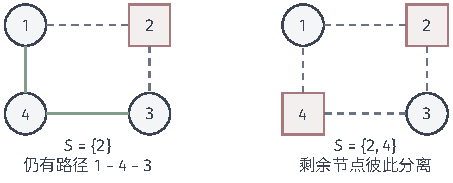
\includegraphics[width=76.652mm]{figures/06-probabilistic-graphical-models/01-representation/tikz/pgm-undirected-separation/figure.pdf}
  \caption{四节点环上的删除检测。方形节点属于条件集合$S$，与它们相接的虚线边一起删除，其余实线边保留。左侧只删$2$，仍可沿$1-4-3$连接；右侧删$2,4$，使$1,3$进入不同连通分量。}
  \label{fig:pgm-undirected-separation}
\end{figure}

\subsection{图分离的检测}
\label{sec:pgm-undirected-separation-test}

删除节点的判据虽然直观，但对有几十上百个节点的图，靠肉眼逐条数路径既慢又容易遗漏，因此需要一个确定的算法把“是否还连通”自动判定出来。做法正是在删去$S$后的诱导子图$\mathcal{G}[V\setminus S]$中，从$A$的全部节点出发搜索：从$A$的全部节点启动广度优先搜索，即可检查剩余连通性。搜索若到达$B$中的节点，就找到一条避开$S$的路径，说明未被分离；若搜索结束仍未到达$B$，则$S$构成分离集。每次扩张都沿保留的节点和边进行，所以访问集恰好覆盖与$A$有剩余路径的节点，这给出算法的正确性依据。采用邻接表和标记数组时，最坏时间为$O(d+|E|)$，额外空间为$O(d)$。这一开销针对结构查询，只回答“路径是否存在”；概率数值计算还要另外处理模型的局部函数与状态汇总。

\subsection{图分离的可靠性与模型类完备性}
\label{sec:pgm-undirected-separation-soundness-completeness}

图分离需要与概率独立严格对应，这种对应包含两个相反方向。\termalias{pgm-soundness}{可靠性}（soundness）要求图上读出的分离对所有按该图构造的分布都保证独立：只要$S$分离$A,B$，相容分布类中的每个分布都满足$\bm{X}_A\perp\bm{X}_B\mid\bm{X}_S$。\term{完备性}（completeness）则要求，对每一项未分离的查询，都至少存在一个相容分布让两端表现出依赖，这样的分布称为依赖见证。两个方向都成立时，图分离恰好刻画模型类强制的独立性：分离的一定独立，未分离的确实可能相关。具体参数仍可能产生图未强制的额外独立；完备性只保证存在依赖的分布，不保证每个分布都依赖。

为了说明具体参数如何带来额外独立，需要先构造由局部权重组成的分布。有向边有明确方向，每个局部表是给定父节点后的条件概率，可以逐行归一化为$1$；无向边没有方向，不能把一条边的一端说成条件于另一端，局部表也不能单独解释成条件分布。无向模型给局部变量组合的状态指定非负权重，所得函数称为\term{势函数}（potential function），简称势。势表达局部取值的相容程度，自身不要求是概率：值越大表示越相容，取$0$表示该局部组合被禁止。将一个完整配置涉及的各团权重相乘，得到未归一化总权重；再除以全部配置的权重总和得到概率。有限离散情形下，这个总和称为\term{配分函数}（partition function）$Z$，要求$Z>0$且有限；归一化由全局总和统一完成，单个局部势只记录相对权重。下面用常数势产生图未要求的独立性。

\begin{example}[不分离不强迫固定分布相关]
  \label{ex:pgm-undirected-fixed-distribution-extra-independence}
  考虑节点集$V=\{1,2\}$、边集$E=\{\{1,2\}\}$的无向图，并令$X_1,X_2\in\{-1,+1\}$。在唯一的二节点团上取常数边势
  \[
    \psi_{\{1,2\}}(x_1,x_2)=1.
  \]
  常数势给四个完整配置同样的权重$1$，总权重为$Z=1+1+1+1=4$。于是各配置的概率都是$p(x_1,x_2)=1/4$，得到一个严格正的联合分布。两个变量各自均匀取值，故对任意$x_1,x_2$，
  \[
    p(x_1,x_2)=\frac14
    =\frac12\cdot\frac12
    =p(x_1)p(x_2),
  \]
  即$X_1\perp X_2$。图中的边保留了两端发生相互作用的可能，常数势却没有使用这种相互作用。因而空集虽然无法分离两个端点，这组参数仍使二者独立。完备性要回答的是同一模型类中能否找到使二者依赖的参数；这个均匀分布只说明，选定参数可以带来图结构之外的独立性。
\end{example}

\begin{theorem}[团因子分解分布上的分离可靠性]
  \label{thm:pgm-undirected-factorization-to-global}
  设$\mathcal{G}=(V,E)$为有限简单无向图，节点$i\in V$取值于可测空间$(\mathcal{X}_i,\mathcal{A}_i)$，其上给定$\sigma$有限基准测度$\mu_i$；记$\mathcal{X}=\prod_{i\in V}\mathcal{X}_i$及$\mu=\bigotimes_{i\in V}\mu_i$，有限离散情形取计数测度。令$\mathcal{C}$为$\mathcal{G}$的有限团族，且对每个$C\in\mathcal{C}$，$\psi_C:\mathcal{X}_C\to[0,\infty)$是可测函数，其中$\mathcal{X}_C=\prod_{i\in C}\mathcal{X}_i$。若$p$相对于$\mu$的密度满足
  \[
    \begin{aligned}
      p(\bm{x})
      &=\frac{1}{Z}\prod_{C\in\mathcal{C}}\psi_C(\bm{x}_C)
        &&\text{$\mu$几乎处处},\\
      Z
      &=\int_{\mathcal{X}}\prod_{C\in\mathcal{C}}
        \psi_C(\bm{x}_C)\,\mathrm{d}\mu(\bm{x}),
        &&0<Z<\infty,
    \end{aligned}
  \]
  则对任意两两不交且$A,B$非空的$A,B,S\subseteq V$，若$S$在$\mathcal{G}$中分离$A$与$B$，就有
  \[
    \bm{X}_A\perp\bm{X}_B\mid\bm{X}_S.
  \]
  势函数可以取零，不要求$p$严格为正。
\end{theorem}

这个可靠性方向的证明要用到“联合分布由团势相乘构成”这一具体形式：图中的分离使团势落在条件集的两侧，分别归一化这两组势，再消去$A\cup B\cup S$以外的变量，就能得到条件概率的乘积。由于下一节才正式给出因子分解，完整证明放到第~\ref{sec:pgm-undirected-factorization-to-markov}节。下面先处理相反的完备性方向：沿一条未被阻断的路径构造依赖，证明模型类中确实存在使两端相关的分布。

\Needspace{14\baselineskip}
\begin{theorem}[严格正二值成对势模型类中的分离完备性]
  \label{thm:pgm-undirected-separation-completeness}
  设$\mathcal{G}=(V,E)$为有限简单无向图，每个节点$i\in V$对应二值随机变量$X_i\in\{-1,+1\}$，且$A,B,S\subseteq V$两两不交、$A,B$非空。若$S$在$\mathcal{G}$中不分离$A$与$B$，则存在一个严格正且按$\mathcal{G}$分解的成对势模型
  \[
    p(\bm{x})=\frac{1}{Z}
      \prod_{\{i,j\}\in E}\psi_{\{i,j\}}(x_i,x_j),
    \qquad \psi_{\{i,j\}}(x_i,x_j)>0,
  \]
  使$\bm{X}_A\not\perp\bm{X}_B\mid\bm{X}_S$。
\end{theorem}

\begin{proof}
从$A$到$B$存在一条避开$S$的路径；去掉路径中重复的节点，可取简单路径
\[
  v_0-v_1-\cdots-v_m,
  \qquad v_0\in A,\quad v_m\in B.
\]
取任意实数$J\neq0$。对路径上的边设
\[
  \psi_{\{v_{r-1},v_r\}}(x_{v_{r-1}},x_{v_r})
  =\exp(Jx_{v_{r-1}}x_{v_r}),
  \qquad r=1,\ldots,m,
\]
其余边的势取常数$1$。这样只让选定路径传递相互作用。所有势严格为正，状态空间有限，故$0<Z<\infty$，所得联合分布属于定理要求的模型类。

为了把这些边权写成转移概率，先固定前一节点的状态$a\in\{-1,+1\}$，对下一状态$b$求和：
\[
  \sum_{b\in\{-1,+1\}}\exp(Jab)
  =e^J+e^{-J}=2\cosh J,
  \qquad \cosh J=\frac{e^J+e^{-J}}{2}.
\]
这个和与$a$无关。对整条路径的权重求和时，可以先消去末端$v_m$，得到因子$2\cosh J$；再消去$v_{m-1}$，又得到同一个因子。依次消去$m$个末端变量后，只剩起点$v_0$的两种状态，所以路径总权重为$2(2\cosh J)^m$。因此
\[
  K(a,b)=\frac{\exp(Jab)}{2\cosh J}
\]
对每个$a$都满足$\sum_bK(a,b)=1$，可以作为下一状态的条件分布。以概率$1/2$选择起点，再逐步使用$K$，所得路径概率正好是原边势乘积除以它的总权重。这里的逐步归一化依赖这条特殊链及其与$a$无关的行和，不能推广为任意无向图上的各势独自归一化。

路径外的变量仅出现在常数势中，因而独立且均匀；连接路径内外的边也没有引入额外作用。完整联合分布由路径分布和路径外的均匀分布相乘得到。由于$\bm{X}_S$都位于路径外，给定它的取值后，路径分布保持原样：对每个$\bm{s}$，
\[
  p(x_{v_0},\ldots,x_{v_m}\mid\bm{s})
  =\frac12\prod_{r=1}^{m}
    \frac{\exp(Jx_{v_{r-1}}x_{v_r})}{2\cosh J}.
\]

把路径分布按相邻节点写成转移概率后，初始状态均匀，每一步都保留相同的耦合。为计算它在均值上的作用，记双曲正切
\[
  \tanh J=\frac{e^J-e^{-J}}{e^J+e^{-J}}.
\]
实数$J\neq0$使分子非零，因而$\rho=\tanh J\neq0$。固定前一状态$a$时，二值条件均值直接算为
\[
  \sum_{b\in\{-1,+1\}}bK(a,b)
  =a\frac{e^J-e^{-J}}{e^J+e^{-J}}
  =a\rho.
\]
所以相邻节点的条件均值满足
\[
  \mathbb{E}[X_{v_r}\mid X_{v_{r-1}}]
  =\rho X_{v_{r-1}}.
\]
转移核乘积还说明，给定$X_{v_0},\ldots,X_{v_{r-1}}$的整段历史后，下一状态的条件分布仍只依赖$X_{v_{r-1}}$。令$c_r=\mathbb{E}[X_{v_0}X_{v_r}]$，先对最后一个变量取条件期望，就有
\[
  \begin{aligned}
    c_r
    &=\mathbb{E}\!\left[
        X_{v_0}\mathbb{E}[X_{v_r}\mid
        X_{v_0},\ldots,X_{v_{r-1}}]\right]\\
    &=\rho\,\mathbb{E}[X_{v_0}X_{v_{r-1}}]
      =\rho c_{r-1}.
  \end{aligned}
\]
起点满足$c_0=\mathbb{E}[X_{v_0}^2]=1$，重复这一步便得到$c_m=\rho^m$。起点的均值为零，而$\mathbb{E}[X_{v_r}]=\rho\mathbb{E}[X_{v_{r-1}}]$，所以路径上各节点的均值也都为零。给定路径外的$\bm{X}_S$不改变这些矩。沿路径逐次取条件期望，每经过一条边便多乘一个耦合系数，因此得到
\[
  \mathbb{E}[X_{v_0}X_{v_m}\mid\bm{X}_S=\bm{s}]
  =\rho^m\neq0,
  \qquad
  \mathbb{E}[X_{v_0}\mid\bm{s}]
  =\mathbb{E}[X_{v_m}\mid\bm{s}]=0.
\]
两个端点的条件均值都是零，而乘积的条件均值非零，因此给定$\bm{X}_S$后仍有依赖。若$\bm{X}_A\perp\bm{X}_B\mid\bm{X}_S$，从两侧各取一个分量便应得到$X_{v_0}\perp X_{v_m}\mid\bm{X}_S$，与上述计算矛盾。选定的非零耦合由此提供了完备性所需的见证分布；换成零耦合，即$J$取零，同一张图也能表示独立分布。
\end{proof}

\section{无向图中的因子分解}
\label{sec:pgm-undirected-factorization}

给定一张无向图，相容的联合分布可以写成一组只依赖局部变量的小函数：图中缺边和分离约束变量间的依赖，具体配置的概率则由数值决定。无向图通过团上的非负权重描述局部相容关系，将这些权重相乘并做一次全局归一化后得到联合分布。这一表示引出两个方向的问题：若分布已经写成团上局部函数的乘积，它是否满足图读出的条件独立；反过来，若分布满足图的全部Markov独立性，是否总能找到这样一组团势表示它。本节先说明团势怎样组织与计算，再依次证明这两个方向，并检查逆向结论在零概率配置和连续变量上的成立条件。

\subsection{因子分解的定义}
\label{sec:pgm-undirected-factorization-definition}

沿用前面的局部权重，为图中每个选定团指定一个势：设$\mathcal{C}$是团的一个族，$\psi_C(\bm{x}_C)$是团$C$上的有限非负函数。将这些势相乘，若能找到$0<Z<\infty$使
\begin{equation}
  p(\bm{x})=\frac{1}{Z}\prod_{C\in\mathcal{C}}\psi_C(\bm{x}_C),
  \label{eq:pgm-undirected-factorization}
\end{equation}
则称$p$按照$\mathcal{G}$进行团因子分解。每个势的自变量来自一个团，实际取值可以只受其中部分变量影响；例如常数势完全不使用团内变量的状态。

势的乘积给出的是一组相对权重，还不是概率：所有配置的权重加起来一般不等于$1$。除以$Z$正是为了把它们等比例缩放成一个合法分布，使全部配置的概率之和为$1$；缩放不改变任意两个配置概率的比值。在离散状态空间上，归一化需要遍历完整配置，将相乘后的权重累加：
\begin{equation}
  Z=\sum_{\bm{x}\in\mathcal{X}}\prod_{C\in\mathcal{C}}\psi_C(\bm{x}_C),
  \qquad
  \mathcal{X}=\prod_{i\in V}\mathcal{X}_i.
  \label{eq:pgm-undirected-partition}
\end{equation}
有限状态空间上，这个有限和给出有限的$Z$；只要至少一个配置权重非零，便有合法的概率分布。可数无限状态空间还需要求和级数收敛。势$\psi_C$记录相对权重，其自身的总和可以异于$1$。不同团共享变量，局部各自归一化后，相乘的函数仍需要全局归一化常数$Z$。

可以用三个二值变量看清最后一点。取两个重叠团$\{1,2\}$与$\{2,3\}$，令两张势表的每项都为$1/4$。每张表按自己的四种配置求和均为$1$，但完整配置共有八种，每种配置的乘积权重为$1/16$，于是
\[
  \sum_{x_1,x_2,x_3}
    \psi_{\{1,2\}}(x_1,x_2)\psi_{\{2,3\}}(x_2,x_3)
  =8\cdot\frac{1}{16}=\frac12.
\]
共享的$x_2$在完整配置中只取一次值，不能把这个求和拆成两张表各自总和的乘积。本例仍需用$Z=1/2$归一化，最终八种配置的概率均为$1/8$。这里按整张团表归一化，与有向条件表在每个父配置下对子状态求和为$1$不同；后者才允许沿无环顺序逐层消去归一化因子。

全局归一化的代价取决于怎样组织求和。若$d$个变量各有$q$个状态，式~\eqref{eq:pgm-undirected-partition}的直接枚举要计算$q^d$项：$20$个二值变量就有$2^{20}=1048576$种配置。链、树或树宽较小的图能让不同配置共享部分计算，从而降低相对于枚举的开销；精确推断章节将说明如何利用这种结构。

全局归一化看似要求把所有配置的权重都算一遍，但有一类查询可以局部完成。给定其余所有变量、只问$X_i$的条件分布时，条件概率是$X_i$各取值权重的相对比值，全局$Z$会在比值中约掉。记未归一化权重为$w(\bm{x})=\prod_{C\in\mathcal C}\psi_C(\bm{x}_C)$，固定$\bm{x}_{-i}=\bm{x}_{V\setminus\{i\}}$，取$p(\bm{x}_{-i})>0$的条件事件。条件概率的分子与分母都带有同一个全局常数：
\begin{equation}
  \begin{aligned}
    p(x_i\mid\bm{x}_{-i})
      &=\frac{w(x_i,\bm{x}_{-i})/Z}
        {\sum_{a\in\mathcal X_i}w(a,\bm{x}_{-i})/Z}\\
      &=\frac{\prod_{C\ni i}\psi_C(\bm{x}_C)}
        {\sum_{a\in\mathcal X_i}
          \prod_{C\ni i}\psi_C(a,\bm{x}_{C\setminus\{i\}})}.
  \end{aligned}
  \label{eq:pgm-undirected-local-conditional}
\end{equation}
在这个比值中，$Z$和所有不含$i$的势都被约去，分母只保留涉及$X_i$的势。记号$\psi_C(a,\bm{x}_{C\setminus\{i\}})$表示将第$i$个变量置为$a$，其余坐标使用已给定的值。二值节点因此只需把两项权重归一化。这个简化利用了其余变量全部已知的条件；若只有少数证据，未观测变量仍需边缘化，通常会留下更大的求和。

任意团都包含于某个极大团，因此小团势可以乘入一个包含它的极大团势。给每个小团选择一次归属，就能将所有势整理为仅以极大团为索引的乘积，同时保持原来的联合分布。“按团分解”与“按极大团分解”由此表示同一分布族，参数组织可以不同。团的阶数则影响所能表示的作用：一般的三节点团势包含三者共同取值的影响，单点势与成对势的乘积未必能表示它。

当势严格为正时，取对数可以把“各团权重相乘”改写成“各项相加”，这在求导、做优化以及借用统计物理语言时都方便得多。令$\varepsilon_C=-\log\psi_C$（势越大，这个量越小），并定义\term{能量函数}（energy function）$E(\bm{x})=\sum_C\varepsilon_C(\bm{x}_C)$为各团“代价”之和，便有
\[
  p(\bm{x})=Z^{-1}\exp[-E(\bm{x})].
\]
指数形式将相乘的相容权重改为相加的能量，较低能量对应较大权重。零势可记作$\varepsilon_C=+\infty$，以表示被禁止的配置；后面需要计算有限对数差分的证明则限于严格正势。

连续变量将求和换成积分。指定各坐标上的$\sigma$有限基准测度$\mu_i$，联合基准测度为$\mu=\bigotimes_{i\in V}\mu_i$，实数变量通常取Lebesgue测度；这是第~\ref{sec:pgm-directed-factor-definition}节采用的密度约定。可测势的乘积需要满足
\begin{equation}
  0<Z=\int_{\mathcal{X}}\prod_{C\in\mathcal{C}}
       \psi_C(\bm{x}_C)\,\mathrm{d}\mu(\bm{x})<\infty.
  \label{eq:pgm-undirected-continuous-partition}
\end{equation}
有限且正的积分使式~\eqref{eq:pgm-undirected-factorization}成为归一化密度。这里检查的是整个势乘积：一些单独不可积的势相乘后可以可积，而$\mathbb{R}^d$上的正的常数势乘积仍会有无穷积分。后面的高斯参数化将用精度矩阵的正定性具体表达这项全局条件。

\begin{example}[四节点环上的相容分数]
  \label{ex:pgm-undirected-cycle}
  令$X_i\in\{0,1\}$，四条边上的势相同：
  \[
    \psi_{\{i,j\}}(x_i,x_j)=
    \begin{cases}
      2,&x_i=x_j,\\
      1,&x_i\neq x_j.
    \end{cases}
  \]
  两端状态相同的一条边将权重乘以$2$，不同的边保持权重。对图~\ref{fig:pgm-undirected-factorization-example}中的$\bm{x}=(0,0,1,1)$，四个边势的乘积是$4$，用$Z=82$归一化便得到概率$2/41$。为计算这个常数，将配置按相同边数分类：沿环回到起点时，状态改变次数为偶数，相同边数因此只能是$4,2,0$。表~\ref{tab:pgm-undirected-cycle-weights}据此汇总全部$16$种配置。
  三类权重相加给出$Z=32+48+2=82$。全相同配置的概率为$p(0,0,0,0)=16/82=8/41$，交替配置的概率为$p(0,1,0,1)=1/82$。相容势由此明确了各配置的相对概率；这些数值只用于演示指定势后的计算。
\end{example}

\begin{figure}[htbp]
  \centering
  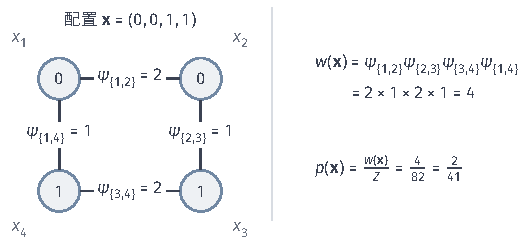
\includegraphics[width=89.701mm]{figures/06-probabilistic-graphical-models/01-representation/tikz/pgm-undirected-factorization-example/figure.pdf}
  \caption{四节点环中配置$\bm{x}=(0,0,1,1)$的权重与概率。四条边的势值相乘为$4$；全部$16$种配置的权重之和为$Z=82$，因此该配置的概率为$2/41$。}
  \label{fig:pgm-undirected-factorization-example}
\end{figure}

\begin{table}[htbp]
  \centering
  \begin{tabular}{crrr}
    \toprule
    相同边数 & 配置数 & 单个权重 & 总权重 \\
    \midrule
    $4$ & $2$ & $16$ & $32$ \\
    $2$ & $12$ & $4$ & $48$ \\
    $0$ & $2$ & $1$ & $2$ \\
    \bottomrule
  \end{tabular}
  \caption{按相同边数汇总四节点二值环的配置。相同边的势为$2$，不同边的势为$1$；各类总权重相加得到配分函数$82$。}
  \label{tab:pgm-undirected-cycle-weights}
\end{table}

\subsection{从因子分解到条件独立性}
\label{sec:pgm-undirected-factorization-to-markov}

删除分离集$S$后，图的连通分量将查询的两组节点隔开。团内节点两两相连，故一个团无法同时跨越这两侧。利用这一点整理团势，就能证明定理~\ref{thm:pgm-undirected-factorization-to-global}中的条件独立性。

\begin{proof}[定理~\ref{thm:pgm-undirected-factorization-to-global}的证明]
取两两不交且被$S$分离的$A,B,S$，其中$A,B$均非空。在$\mathcal{G}[V\setminus S]$中，将所有与$A$相交的连通分量合为$U$，其余节点合为$W=V\setminus(S\cup U)$。这些集合满足$A\subseteq U$、$B\subseteq W$，且$U$与$W$之间无边。

若一个团含有$U$和$W$各一个节点，两节点之间就应有边，这与集合的构造矛盾。因此每个团或者全部在$S$中，或者只涉及$U$与$S$，或者只涉及$W$与$S$。分别将这三类势相乘，联合分布写成
\begin{equation}
  p(\bm{u},\bm{w},\bm{s})
  =Z^{-1}h(\bm{s})f(\bm{u},\bm{s})g(\bm{w},\bm{s}),
  \label{eq:pgm-undirected-separated-factors}
\end{equation}
三组自变量$\bm{u},\bm{w},\bm{s}$分别对应$\bm{X}_U,\bm{X}_W,\bm{X}_S$；某类没有势时，其乘积取$1$。

为了将两侧函数归一化，在离散情形定义$F(\bm{s})=\sum_{\bm{u}}f(\bm{u},\bm{s})$、$G(\bm{s})=\sum_{\bm{w}}g(\bm{w},\bm{s})$；连续情形使用相应乘积测度的积分。取$p_S(\bm{s})$有限且严格为正的条件值，离散情形的所有正概率事件都满足此条件，连续情形中这样的取值承载全部$\bm{X}_S$概率。式~\eqref{eq:pgm-undirected-separated-factors}由此要求$h(\bm{s})$为正。团势非负，Tonelli定理允许先分别积分两侧函数，得到
\[
  p_S(\bm{s})=Z^{-1}h(\bm{s})F(\bm{s})G(\bm{s}).
\]
正且有限的条件密度排除了两侧积分为零或无穷的情形：$F(\bm{s})$或$G(\bm{s})$为零时联合积分为零，一侧积分无穷而另一侧为正时联合积分无穷。所以两侧的$F(\bm{s})$与$G(\bm{s})$均正且有限，条件联合密度成为
\begin{equation}
  p(\bm{u},\bm{w}\mid\bm{s})
  =\frac{f(\bm{u},\bm{s})}{F(\bm{s})}
   \frac{g(\bm{w},\bm{s})}{G(\bm{s})}.
  \label{eq:pgm-undirected-conditional-product}
\end{equation}
右侧各因子分别是两侧的条件密度，这个乘积给出$\bm{X}_U\perp\bm{X}_W\mid\bm{X}_S$。

最后分别消去$U\setminus A$和$W\setminus B$的变量。式~\eqref{eq:pgm-undirected-conditional-product}的两侧仍可独立求和或积分，留下只含$\bm{x}_A,\bm{s}$和只含$\bm{x}_B,\bm{s}$的条件边缘分布。故$\bm{X}_A\perp\bm{X}_B\mid\bm{X}_S$，任意被分离的两组变量都满足所需条件独立性。
\end{proof}

两侧函数的归一化在正概率条件事件或几乎处处的条件密度上完成，所除的常数正且有限。因此团势中的零值也适用于此证明。再结合定理~\ref{thm:pgm-undirected-global-implications}，团分解同时推出局部和成对性质。这个方向直接来自势乘积；下一节的Hammersley--Clifford结论负责相反方向，即从独立性重建团势。

对四节点环，可以直接看到这种两侧归一化。固定示例~\ref{ex:pgm-undirected-cycle}中的$X_2=x_2,X_4=x_4$，将涉及节点1和节点3的边势各自相乘：
\[
  \begin{aligned}
    f(x_1)&=\psi_{\{1,2\}}(x_1,x_2)\psi_{\{1,4\}}(x_1,x_4),\\
    g(x_3)&=\psi_{\{2,3\}}(x_2,x_3)\psi_{\{3,4\}}(x_3,x_4).
  \end{aligned}
\]
两邻居都取零时，即$x_2=x_4=0$，两侧权重满足$f(0)=g(0)=4$和$f(1)=g(1)=1$，因而
\[
  p(x_1,x_3\mid0,0)
  =\frac{1}{25}
    \begin{pmatrix}16&4\\4&1\end{pmatrix}_{x_1+1,x_3+1}.
\]
行与列都按状态$0,1$排列。两侧的条件边缘均为$(4/5,1/5)$，相乘正好得到矩阵的各项。若换成$x_2=0,x_4=1$，$f$与$g$的两种状态权重都为$2$，四个条件联合概率便都为$1/4$。两种条件值产生不同的边缘分布，但每种情况下，给定邻居后的联合分布都由两侧边缘相乘得到。

\subsection{从条件独立性到因子分解}
\label{sec:pgm-undirected-hammersley-clifford}

正向（团乘积$\Rightarrow$独立性）相对直接，逆向（独立性$\Rightarrow$团乘积）则更微妙，也是无向图模型理论的核心：现在只知道联合分布满足图的全部独立性约束，需要为它找到一组团势。构造的思路可以先从直觉上理解：先任意选定一个基准配置作为参照，考察把其中一部分坐标改成当前取值时，对数概率改变了多少；这个改变量原则上可能依赖被改变的任意一组变量。若某一组变量中包含两个在图上不相邻的节点，缺边所要求的条件独立就会保证“它们的联合改变没有额外贡献”，对应的交互项必然为零。于是能留下非零贡献的变量组，恰好都是两两相连的团。下面用Gill笔记中的Möbius交替差分把这一构造严格完成\scite{pgm-undirected-gill2011}。

\term{Hammersley--Clifford定理}在有限离散、严格正的情形下给出独立性与团分解的等价关系。严格正的范围是完整的笛卡尔积$\mathcal{X}=\prod_i\mathcal{X}_i$：每个配置都须满足$p(\bm{x})>0$，范围覆盖各坐标状态组合出的全部配置。定理~\ref{thm:pgm-undirected-markov-equivalence}已证明三种Markov性质在这些条件下等价，所以只需从其中一种构造团势。

\begin{theorem}[有限离散Hammersley--Clifford定理]
  \label{thm:pgm-undirected-hammersley-clifford}
  设$\mathcal{G}=(V,E)$为有限简单无向图，每个节点$i\in V$对应取值于有限非空状态空间$\mathcal{X}_i$的随机变量$X_i$。令$p$为$\bm{X}=(X_i)_{i\in V}$在乘积状态空间$\mathcal{X}=\prod_{i\in V}\mathcal{X}_i$上的联合质量函数，并且$p(\bm{x})>0$对所有$\bm{x}\in\mathcal{X}$成立。则以下四个条件等价：$p$满足相对于$\mathcal{G}$的全局Markov性质；$p$满足相对于$\mathcal{G}$的局部Markov性质；$p$满足相对于$\mathcal{G}$的成对Markov性质；$p$能按$\mathcal{G}$的团分解。分解中的势可以全部取为严格正值。
\end{theorem}

\begin{proof}
团分解到全局性质的方向由定理~\ref{thm:pgm-undirected-factorization-to-global}给出，三种Markov性质的等价由定理~\ref{thm:pgm-undirected-markov-equivalence}给出。剩下的任务是从成对性质重建分布。任选基准配置$\bm{x}^{\circ}\in\mathcal{X}$，对每个$D\subseteq V$，记
\[
  \bm{x}^{D}=(\bm{x}_D,\bm{x}^{\circ}_{V\setminus D}),
  \qquad
  L_D(\bm{x}_D)=\log p(\bm{x}^{D}).
\]
配置只在$D$中的坐标使用当前值，其他坐标都取基准值。每个配置概率严格为正，所以这些对数可作为有限实数参与后面的加减。

改变一组变量$D$引起的对数概率变化，既可能来自这些变量各自的单独作用，也可能来自它们之间的交互作用。要单独留下“$D$中变量同时改变才产生”的那部分，就要把只改变其中更小子集时的贡献逐一扣掉：加回单变量项、再扣掉被多减的部分，如此交替进行，这正是容斥的做法。为分离出每个坐标子集的作用，对每个$D\subseteq V$构造
\begin{equation}
  \phi_D(\bm{x}_D)
  =\sum_{B\subseteq D}(-1)^{|D|-|B|}L_B(\bm{x}_B).
  \label{eq:pgm-undirected-mobius}
\end{equation}
常数项为$\phi_{\varnothing}=\log p(\bm{x}^{\circ})$。这种\term{Möbius分解}（Möbius decomposition）用交替加减剔除较小子集的作用，留下同时改变$D$中各坐标时额外产生的部分。单节点项和二节点项分别为
\[
  \begin{aligned}
    \phi_{\{i\}}&=L_{\{i\}}-L_{\varnothing},\\
    \phi_{\{i,j\}}
      &=L_{\{i,j\}}-L_{\{i\}}-L_{\{j\}}+L_{\varnothing}.
  \end{aligned}
\]

验证这些局部项是否保留了完整分布，可将所有$D$的项重新相加。交换两层有限求和，得到
\begin{align}
  \sum_{D\subseteq V}\phi_D(\bm{x}_D)
  &=\sum_{B\subseteq V}L_B(\bm{x}_B)
      \sum_{D:\,B\subseteq D\subseteq V}(-1)^{|D|-|B|}
      \notag\\
  &=L_V(\bm{x}_V)=\log p(\bm{x}).
  \label{eq:pgm-undirected-mobius-inversion}
\end{align}
为计算固定$B$对应的内层系数，将包含$B$的每个$D$唯一写成$D=B\cup K$，其中$K\subseteq V\setminus B$。此时$|D|-|B|=|K|$，而从$V\setminus B$中选出$k$个额外节点有$\binom{|V\setminus B|}{k}$种方式，所以
\[
  \begin{aligned}
    \sum_{D:\,B\subseteq D\subseteq V}(-1)^{|D|-|B|}
    &=\sum_{k=0}^{|V\setminus B|}
        \binom{|V\setminus B|}{k}(-1)^k\\
    &=(1-1)^{|V\setminus B|}.
  \end{aligned}
\]
$B\neq V$时，额外节点的子集所给出的正负项相消，该系数为零；$B=V$时只剩$K=\varnothing$对应的唯一一项$1$。因此最终仅保留完整配置的对数概率。

成对性质随后决定哪些局部项留下。非空子集$D$若不是团，其内就有不相邻节点$i,j$；令$R=V\setminus\{i,j\}$。固定任意$\bm{x}_R$时，两节点的条件联合概率由各自条件边缘相乘得到。对任意$a,a'\in\mathcal{X}_i$和$b,b'\in\mathcal{X}_j$，先在这个条件分布内比较四个取值：
\[
  \begin{aligned}
    &p(a,b\mid\bm{x}_R)p(a',b'\mid\bm{x}_R)\\
    &\quad=p(a\mid\bm{x}_R)p(a'\mid\bm{x}_R)
            p(b\mid\bm{x}_R)p(b'\mid\bm{x}_R)\\
    &\quad=p(a,b'\mid\bm{x}_R)p(a',b\mid\bm{x}_R).
  \end{aligned}
\]
两边的四个条件边缘因子完全相同，只是组合次序不同。每个条件联合概率乘以$p(\bm{x}_R)$就恢复联合概率，因此两侧同乘$p(\bm{x}_R)^2$，得到
\begin{equation}
  \begin{aligned}
    &p(a,b,\bm{x}_R)p(a',b',\bm{x}_R)\\
    &\qquad=p(a,b',\bm{x}_R)p(a',b,\bm{x}_R).
  \end{aligned}
  \label{eq:pgm-undirected-rectangle}
\end{equation}
也可以从联合概率除以$p(\bm{x}_R)$的条件化公式反向核对：两边的归一化因子相同，可以约去。严格正性使这个条件事件的概率为正。取$a=x_i,a'=x_i^{\circ},b=x_j,b'=x_j^{\circ}$，使$R$中一个子集$B$使用当前值，其余坐标使用基准值。取有限对数后，有
\[
  L_{B\cup\{i,j\}}-L_{B\cup\{i\}}
  -L_{B\cup\{j\}}+L_B=0.
\]
这个零差分说明，其他坐标固定时，两非邻居的联合变化可以完全由各自的变化解释。

令$T=D\setminus\{i,j\}$。在式~\eqref{eq:pgm-undirected-mobius}中，先固定$B\subseteq T$。原来求和中的四个子集是$B$、$B\cup\{i\}$、$B\cup\{j\}$和$B\cup\{i,j\}$；它们含有相同的其他节点，只在是否纳入$i,j$上不同。由于$|D|=|T|+2$，这四项在提出共同系数$(-1)^{|T|-|B|}$后，符号依次为$+,-,-,+$。因此按子集是否含有$i,j$将求和项分为四组，再把同一个$B$的四项放在一起，便对应刚才的矩形差分：
\begin{equation}
  \begin{aligned}
    \phi_D
    =\sum_{B\subseteq T}(-1)^{|T|-|B|}
      \bigl(&L_{B\cup\{i,j\}}-L_{B\cup\{i\}}\\
            &-L_{B\cup\{j\}}+L_B\bigr)=0.
  \end{aligned}
  \label{eq:pgm-undirected-nonclique-vanishes}
\end{equation}
每个括号都为零，故只要一个子集含有非邻接对，它的整个交互项就为零。这一步同时排除了涉及这对节点的所有更高阶项。

留下的非空子集全是团，记其族为$\mathcal{C}_{\mathrm{all}}$。令$\psi_C=\exp(\phi_C)>0$，将式~\eqref{eq:pgm-undirected-mobius-inversion}的和指数化，得到
\[
  p(\bm{x})
  =\exp(\phi_{\varnothing})
     \prod_{C\in\mathcal{C}_{\mathrm{all}}}\psi_C(\bm{x}_C).
\]
联合概率对$\bm{x}$求和为一，所以团势乘积的配分函数是$Z=\exp(-\phi_{\varnothing})$，正且有限。若需仅保留极大团，进一步将每个小团势并入一个包含它的极大团即可。
\end{proof}

Möbius恒等式负责重建对数概率，成对独立性负责消去非团项，两者共同给出团分解。严格正性使每个其余变量配置都能用于条件化，也使矩形等式的对数有限。这是逆向结论在整类分布上成立的充分条件。沿用四节点环，下面给出一个带零概率的分布：它满足所有Markov独立性，却无法按团分解，从而展示严格正性所保护的方向。

\begin{example}[满足全局Markov性质却不能团分解]
  \label{ex:pgm-undirected-zero-support}
  在同一四节点环上，用两个相互独立的公平二值变量$U,V$构造分布：
  \[
    X_1=U,\quad X_2=V,\quad
    X_3=U\mathbin{\oplus}V,\quad X_4=U,
  \]
  $\oplus$表示模$2$加法。两变量的四种取值分别生成表~\ref{tab:pgm-undirected-zero-support}中的四个配置，其他完整配置的概率均为零。
\end{example}

\begin{table}[htbp]
  \centering
  \begin{tabular}{ccccc}
    \toprule
    $x_1$ & $x_2$ & $x_3$ & $x_4$ & 概率 \\
    \midrule
    $0$ & $0$ & $0$ & $0$ & $1/4$ \\
    $0$ & $1$ & $1$ & $0$ & $1/4$ \\
    $1$ & $0$ & $1$ & $1$ & $1/4$ \\
    $1$ & $1$ & $0$ & $1$ & $1/4$ \\
    \bottomrule
  \end{tabular}
  \caption{四节点环中四个正概率配置。给定任意一对对角节点即可确定所在行；边上的取值对允许的组合则多于这个全局支持集。}
  \label{tab:pgm-undirected-zero-support}
\end{table}

先检验独立性。给定$(X_2,X_4)$便知道$(U,V)$，$X_1$与$X_3$都成为常量，所以二者条件独立。给定$(X_1,X_3)$也能确定$(U,V)$，从而$X_2\perp X_4\mid(X_1,X_3)$。四节点环删除一个节点仍连通，非空节点集间的非平凡分离只可能是用一对对角节点隔开另一对。这两项条件独立因此覆盖全局Markov性质要求的所有查询，局部和成对性质也随之成立。

再检验能否分解。假设已有四个边势，单点势可先乘入某个关联的边势。取零概率配置$\bm{y}=(0,0,1,0)$：边$\{1,2\}$的取值$(0,0)$在正概率配置$(0,0,0,0)$中出现；边$\{2,3\}$的取值$(0,1)$在$(1,0,1,1)$中出现；边$\{3,4\}$的取值$(1,0)$在$(0,1,1,0)$中出现；边$\{1,4\}$的取值$(0,0)$则又在$(0,0,0,0)$中出现。每个正概率配置都要求其边势乘积为正，所以上述四个边势值全部为正。在$\bm{y}$处相乘便会给出$p(\bm{y})>0$，与指定的零概率矛盾。

图~\ref{fig:pgm-undirected-zero-support}将这四个取值对标在环的边上。局部投影各自允许这些取值，拼成的完整配置却不属于表~\ref{tab:pgm-undirected-zero-support}的支持集。
\begin{figure}[htbp]
  \centering
  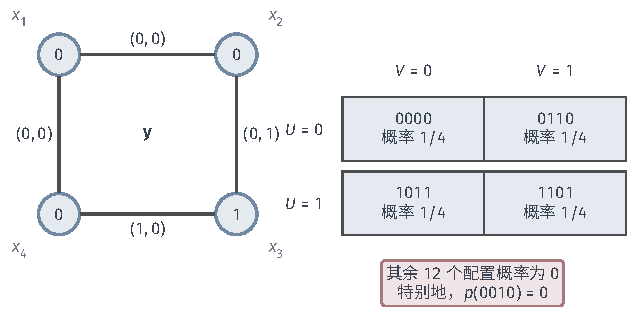
\includegraphics[width=106.825mm]{figures/06-probabilistic-graphical-models/01-representation/tikz/pgm-undirected-zero-support/figure.pdf}
  \caption{全局Markov性质成立而团分解失败的零概率反例。左侧配置$\bm y=(0,0,1,0)$的每个边取值对都出现在正概率配置中；右侧$2\times2$表按$(U,V)$列出四个正概率配置，其余12个配置的概率为0。边势若表示这些正概率配置，$\bm y$处的各势值也须为正，故无法同时满足$p(\bm y)=0$。}
  \label{fig:pgm-undirected-zero-support}
\end{figure}

这个分布的条件独立来自条件变量对其余变量的完全确定。其全局支持约束却超出了边势能表达的范围：四个局部允许的取值对可以拼成一个全局禁止的配置。上述矛盾直接排除了非负团势分解。零概率分布中也有可分解的情形，例如边势$\mathbf{1}\{x_i=x_j\}$能用局部零值施加相等约束；有零值时，逆向分解是否成立取决于具体支持结构。

对连续密度，基准配置构造还遇到逐点值的问题。若只知道$p>0$几乎处处，一个预先固定的坐标截面可能属于零测集，而密度在这样的集合上可任意修改。这会影响在截面上定义$L_D$的逐点推理。一般可测空间中的逆向定理需要处理这些例外集合及密度版本\scite{pgm-lauritzen1996}。

例如，在二维域$(0,1)^2$上取均匀密度$p(x_1,x_2)=1$，再选择下面这个版本：
\[
  \widetilde p(x_1,x_2)=
  \begin{cases}
    0,&x_2=1/2,\\
    1,&x_2\neq1/2.
  \end{cases}
\]
直线$x_2=1/2$的二维Lebesgue测度为零，所以两种密度给出同一个联合分布，且$\widetilde p>0$几乎处处。可是取基准配置$\bm{x}^{\circ}=(1/2,1/2)$、令$D=\{1\}$时，$\bm{x}^{D}=(x_1,1/2)$始终落在这条直线上。沿这个截面读取的$L_D=\log\widetilde p(x_1,1/2)$不再是有限实数，不能直接放入前面的有限对数差分。这不否认该分布有良好的连续版本，而是说明不能对任意密度版本都任取基准截面作逐点推理。

连续性可提供一个便于核验的充分条件。令$\mathcal{X}=\prod_i I_i$，其中$I_i$均为非空开区间，取Lebesgue乘积测度；设$p$连续、处处严格正，且积分为$1$。满足成对Markov性质时，存在连续严格正的团势，其乘积等于$p$乘以一个有限正数。

为证明这一点，先固定一对不相邻节点$i,j$，记其余坐标为$R$。条件独立首先是在$\bm{X}_R$的分布$P_R$几乎处处的条件值上成立。由$p$处处正，对$a,b$积分得到的边缘密度$p_R$也为正；其总积分为$1$，又保证它在Lebesgue几乎处处有限。因此$p_R$在Lebesgue几乎处处正且有限。在这部分条件值上，$P_R$零概率集合也必为Lebesgue零测集：若一个集合具有正的Lebesgue测度，对其上的正函数$p_R$积分就会得到正概率。这样，条件独立关系可以在Lebesgue几乎处处的条件值$\bm r$上使用。此时条件联合密度按两侧边缘相乘，因而对Lebesgue几乎处处的$(a,b)$有
\[
  p(a,b,\bm r)
  =p_R(\bm r)\,p(a\mid\bm r)\,p(b\mid\bm r).
\]
利用Fubini定理，可以在$(a,a',b,b')$的乘积空间中去掉四个配对各自的零测例外，使$(a,b)$、$(a',b')$、$(a,b')$、$(a',b)$的上述分解同时成立。两边相乘后，各个条件边缘因子和$p_R(\bm r)^2$相同，就得到式~\eqref{eq:pgm-undirected-rectangle}。再对$\bm r$使用Fubini定理，便知该矩形等式相对于$(a,a',b,b',\bm{x}_R)$的Lebesgue乘积测度几乎处处成立。

矩形等式两侧之差连续，若有一点非零，便会在该点某个正测度邻域中非零，与几乎处处相等矛盾。矩形等式因而处处成立，可以选取任意域内基准配置，再应用有限节点集合的Möbius分解。这里有限的是节点数，子集求和仍只有有限项，并不要求各个连续状态空间有限。团势乘积与$p$成正比例，可积性也随之得到保证。

上述连续性只用于将几乎处处的矩形等式推广为逐点等式，一般可测版本可以采用其他条件。若要进一步利用$\log p$的混合偏导，则还需相应的可微性，例如二阶连续可微。实际建模时选定光滑势或神经参数化势后，也须检查整个乘积的可积性；存在某组团函数的分解定理，并未替具体函数族及参数完成这项检查。

\section{局部参数化}
\label{sec:pgm-undirected-local-parameterization}

前面的因子分解只说明联合分布“可以写成团势乘积”，但势函数仍是抽象的非负函数，还不能直接拿去计算或从数据中学习。要让模型真正可用，需要给每个团势指定具体的数学形式，并用一组可调的数值参数来描述它，这一步称为局部参数化。离散变量可以直接用表格，或用配置特征的加权组合；连续变量则常取二次函数，使积分与条件分布都有闭式解。无论采用哪种形式，都必须满足同一个全局约束：所有势相乘后能被一个正且有限的常数归一化，否则它根本不定义概率分布。

\subsection{离散变量的局部参数化}
\label{sec:pgm-undirected-discrete-parameterization}

以离散状态的偏好为例，单点势$\psi_{\{i\}}(x_i)$给每个状态指定权重，成对势$\psi_{\{i,j\}}(x_i,x_j)$给状态对指定相容权重，高阶势则记录多个状态组合的额外作用。最直接的表示是势表；每个变量有$q$个状态时，一般的$k$节点团需要$q^k$个表项。增加团的阶数能容纳更丰富的共同作用，也相应增加存储量。

下面的对数线性形式与学习公式都先限制在有限状态空间上，并只使用有限个、取有限实值的固定特征。这样配分函数是有限和，对参数求导时可以逐项计算。可数无限状态空间的扩展仍须另行检查收敛、可微性以及交换求导与求和的条件。

势表虽直观，却把团的每一种配置都当成独立参数，参数数随团的阶数指数增长，也难以表达“所有边都偏好相同标签”这类可共享的规律。更紧凑的做法是挑出若干有意义的局部特征，用它们的加权组合决定势的对数，让一个参数同时控制许多配置。若势严格为正，就可用团内特征$f_{C,r}(\bm{x}_C)$表示它的对数。选择“两个状态相同”或“团取某个配置”等指示特征后，为每个特征指定一个系数：
\[
  \log\psi_C(\bm{x}_C;\bm{\theta})
  =\sum_r\theta_{C,r}f_{C,r}(\bm{x}_C).
\]
将各团特征与系数分别汇总为$\bm{f}(\bm{x})$和$\bm{\theta}$，势乘积就对应特征内积的指数，形成\term{对数线性模型}（log-linear model）：
\begin{equation}
  \begin{aligned}
    p_{\bm{\theta}}(\bm{x})
      &=\exp\{\bm{\theta}^{\top}\bm{f}(\bm{x})-A(\bm{\theta})\},\\
    A(\bm{\theta})
      &=\log\sum_{\bm{x}}
          \exp\{\bm{\theta}^{\top}\bm{f}(\bm{x})\}.
  \end{aligned}
  \label{eq:pgm-undirected-exponential-family}
\end{equation}
参数通过特征内积进入指数，归一化由$A=\log Z$完成，故该模型属于\term{指数族}（exponential family）。为每个团配置都设置一个指示特征，可以表示任意严格正的团势表；减少特征或让多处特征共享系数，可以节省参数，同时缩小图结构允许的分布族\scite{pgm-wainwright2008}。

对数线性模型最简单、也最常用的特例来自统计物理，只用“节点自己的取值”和“相邻两节点取值的乘积”两类特征。\term{Ising模型}用$x_i\in\{-1,+1\}$表示两个状态，分别以状态值和相邻状态乘积为特征：
\begin{equation}
  p(\bm{x})=\frac{1}{Z}
  \exp\left\{\sum_i h_i x_i+
             \sum_{\{i,j\}\in E}J_{i,j}x_i x_j\right\}.
  \label{eq:pgm-undirected-ising}
\end{equation}
单点系数$h_i>0$提高$+1$状态的权重，边系数$J_{i,j}>0$提高相同状态对的权重，$J_{i,j}<0$则提高不同状态对的权重。这些系数控制对数相容分数，边缘概率还由其余势及全局归一化共同确定。把示例~\ref{ex:pgm-undirected-cycle}的状态通过$s_i=2x_i-1$换为$\{-1,+1\}$，原来的边势可写成
\[
  \psi_{\{i,j\}}(x_i,x_j)
  =\sqrt{2}\exp\left\{\frac{\log2}{2}s_i s_j\right\}.
\]
四条边的$\sqrt{2}$相乘只产生一个常数，可并入$Z$。因此该例对应单点系数为零、边耦合为$J_{i,j}=(\log2)/2$的Ising环。

当状态不止两个、而是$q$个类别$x_i\in\{1,\ldots,q\}$时（例如图像有多种区域类别），“取值乘积”不再有定义，但“两个邻居是否属于同一类”仍然有意义。\term{Potts模型}就用类别是否相同作为特征，其常见边势为
\[
  \psi_{\{i,j\}}(x_i,x_j)
  =\exp\{J_{i,j}\mathbf{1}\{x_i=x_j\}\}.
\]
类别编号只用于区分状态，势通过是否相同来奖励或惩罚组合，无需定义类别间的数值距离。更高阶的特征还可表达共同作用：对三个取值为$\{-1,+1\}$的变量，三节点团中的对数势$\lambda x_i x_j x_k$能区分乘积为正与为负的配置。使用该特征需要相应的团结构；在不含该团的图上增加这样的势，一般会改变原来的独立性约束。第~\ref{chap:pgm-energy-models}章继续讨论Ising、Potts及其他能量模型的建模和计算。

势的系数刻画了“相邻变量有多倾向于一致”，但在实际问题中这些系数往往事先并不知道，需要从观测到的完整配置中估计出来。与上一章估计有向条件表的思路一致，可以采用极大似然：固定图和特征函数后，未知量就是系数$\bm{\theta}$，选择使整批观测出现概率最大的系数。全局归一化常数$Z$也依赖$\theta$，这会让优化比逐行归一化的有向条件表更复杂。给定$n$个完整、独立同分布的样本向量$\bm{x}_1,\ldots,\bm{x}_n$，样本独立性给出似然$L(\bm{\theta})=\prod_{k=1}^n p_{\bm{\theta}}(\bm{x}_k)$。取对数并除以$n$，代入对数线性形式，得到
\[
  \begin{aligned}
    \ell(\bm{\theta})
    &=\frac1n\log L(\bm{\theta})\\
    &=\frac1n\sum_{k=1}^n
       \left[\bm{\theta}^{\top}\bm{f}(\bm{x}_k)
             -A(\bm{\theta})\right].
  \end{aligned}
\]
对数是严格递增函数，除以正数$n$也不改变最大化方向。将经验特征均值记为\allowbreak$\overline{\bm{f}}=n^{-1}\sum_{k=1}^n\bm{f}(\bm{x}_k)$，求和中的线性项就成为$\bm{\theta}^{\top}\overline{\bm{f}}$；每条样本共用同一个归一化函数，所以平均后仍减去$A(\bm{\theta})$。

梯度还需要计算归一化函数的导数。记$Z(\bm{\theta})=\exp A(\bm{\theta})$，即当前系数下的配分函数。对第$r$个系数，有限状态空间允许逐项求导，链式法则给出
\[
  \begin{aligned}
    \frac{\partial A}{\partial\theta_r}
    &=\frac1{Z(\bm{\theta})}
       \sum_{\bm{x}}f_r(\bm{x})
          e^{\bm{\theta}^{\top}\bm{f}(\bm{x})}\\
    &=\sum_{\bm{x}}p_{\bm{\theta}}(\bm{x})f_r(\bm{x})
      =\mathbb{E}_{p_{\bm{\theta}}}[f_r(\bm{X})].
  \end{aligned}
\]
第二个等号把指数权重除以$Z$认作模型概率。因此平均对数似然及梯度为
\begin{equation}
  \begin{aligned}
    \ell(\bm{\theta})
      &=\bm{\theta}^{\top}\overline{\bm{f}}-A(\bm{\theta}),\\
    \nabla_{\bm{\theta}}\ell(\bm{\theta})
      &=\overline{\bm{f}}
        -\mathbb{E}_{p_{\bm{\theta}}}[\bm{f}(\bm{X})].
  \end{aligned}
  \label{eq:pgm-undirected-learning-gradient}
\end{equation}
上面的逐项求导说明，梯度的第二项来自归一化函数对参数的导数。它要求将数据中的特征平均与当前联合分布中的特征期望比较；沿最大化方向更新时，某项经验均值高于当前模型期望，就给相应系数一个增大的梯度分量。参数学习因此反复调用推断。式~\eqref{eq:pgm-undirected-local-conditional}的单节点条件归一化解决的是给定其余变量的查询，这里的期望则针对整个联合分布。树上可通过消息计算，一般图的开销取决于消元所形成的中间因子。第~\ref{chap:pgm-elimination}章介绍这类推断，第~\ref{chap:pgm-parameter-learning}章进一步说明它在参数估计中的作用。

\subsection{连续变量的局部参数化}
\label{sec:pgm-undirected-continuous-parameterization}

离散势表解决的是取值为有限类别的变量。对连续变量（例如像素的亮度、温度场），最常用、也最便于精确计算的局部势是二次函数：它把“相邻变量取值相差太大”按平方大小施加惩罚，得到的联合分布正是熟悉的高斯分布，因而均值、协方差和条件分布都有闭式解。\term{高斯Markov随机场}（Gaussian Markov random field, GMRF）就是用无向图表示联合高斯分布的条件独立性，其势乘积能否在整个$\mathbb{R}^d$上归一化，由二次型系数矩阵是否正定决定。先考虑$\mathbb{R}^d$上相对于Lebesgue测度的非退化分布，令
\begin{equation}
  \begin{aligned}
    p(\bm{x})&=Z^{-1}
      \exp\left\{-\tfrac12\bm{x}^{\top}\bm{Q}\bm{x}
                   +\bm{h}^{\top}\bm{x}\right\},\\
    \bm{Q}&=\bm{Q}^{\top}\succ0.
  \end{aligned}
  \label{eq:pgm-undirected-gaussian}
\end{equation}
$\bm{Q}$称为\term{精度矩阵}（precision matrix），是协方差矩阵的逆；在二次型$-\tfrac12\bm{x}^{\top}\bm{Q}\bm{x}$中，它的非对角元$Q_{i,j}$正是连接$i,j$的边势系数，因此$Q_{i,j}=0$就意味着$i,j$之间没有直接的二次耦合。$\bm{h}\in\mathbb{R}^d$控制线性项，相当于整体上对各个取值方向的偏好。为了从这个表达式读出均值和协方差，先解$\bm{Q}\bm{m}=\bm{h}$，得到$\bm{m}=\bm{Q}^{-1}\bm{h}$。利用$\bm{Q}$对称，将指数中的二次式配方为
\[
  \begin{aligned}
    -\tfrac12\bm{x}^{\top}\bm{Q}\bm{x}
      +\bm{h}^{\top}\bm{x}
    ={}&-\tfrac12(\bm{x}-\bm{m})^{\top}
               \bm{Q}(\bm{x}-\bm{m})\\
       &{}+\tfrac12\bm{h}^{\top}\bm{Q}^{-1}\bm{h}.
  \end{aligned}
\]
第一项以$\bm{m}$为中心，第二项不再依赖$\bm{x}$，只影响归一化常数。与标准高斯密度比较，均值为$\bm{m}$，协方差为$\bm{\Sigma}=\bm{Q}^{-1}$。计算积分时，先平移到$\bm{x}-\bm{m}$，再沿$\bm{Q}$的正交特征向量取坐标$\bm{z}$；这两步的体积因子均为$1$。若正特征值为$\lambda_1,\ldots,\lambda_d$，中心二次项的积分分成
\[
  \prod_{i=1}^d\int_{\mathbb{R}}
       e^{-\lambda_i z_i^2/2}\,\mathrm{d}z_i
  =\prod_{i=1}^d\sqrt{\frac{2\pi}{\lambda_i}}
  =(2\pi)^{d/2}\det(\bm{Q})^{-1/2}.
\]
再乘回与$\bm{x}$无关的指数因子，积分得到
\begin{equation}
  Z=(2\pi)^{d/2}\det(\bm{Q})^{-1/2}
     \exp\left\{\tfrac12\bm{h}^{\top}\bm{Q}^{-1}\bm{h}\right\}.
  \label{eq:pgm-undirected-gaussian-partition}
\end{equation}
为什么归一化必须要求$\bm{Q}$正定，可以从几何上理解：把坐标轴旋转到$\bm{Q}$的特征向量方向后，二次型化成$\sum_i\lambda_i z_i^2$。若所有特征值$\lambda_i>0$，权重沿每个方向都按$e^{-\lambda_i z_i^2/2}$衰减，远离原点时迅速趋于零，积分因而有限；这正是正定性的作用。对于这种全空间二次能量，正定性也是必要条件。将坐标轴变换到$\bm{Q}$的特征向量方向后，负特征值会让指数沿相应方向按正二次项增长，权重不衰减反而趋向无穷；零特征值则只留下线性指数或常数，沿该方向既不奖励也不惩罚。在整条实轴上，这两种情形的积分都发散。

展开二次型，就能将单节点项与节点对的作用分开：
\[
  \begin{aligned}
    &-\tfrac12\bm{x}^{\top}\bm{Q}\bm{x}+\bm{h}^{\top}\bm{x}\\
    &\qquad=\sum_i\left(-\tfrac12 Q_{i,i}x_i^2+h_i x_i\right)
             -\sum_{i<j}Q_{i,j}x_i x_j.
  \end{aligned}
\]
记$Q_{i,j}$为$\bm{Q}$的第$(i,j)$个元素。单点项指数化后成为单点势，非零交叉项则成为边势$\exp(-Q_{i,j}x_i x_j)$。这个边势单独可能不可积，其用途是参与全局势乘积，后者由正定性保证可积。所有缺边都满足$Q_{i,j}=0$时，交叉项仅出现在图的边上，得到所需团分解。

无向图关心的是“给定其余全部变量后谁与谁独立”。在高斯分布中，这个问题有一个异常简洁的答案：它由精度矩阵的非对角零元、而不是协方差矩阵的非对角零元决定。非退化高斯分布中，精度的非对角零元恰好对应成对条件独立性：
\begin{equation}
  Q_{i,j}=0
  \quad\Longleftrightarrow\quad
  X_i\perp X_j\mid\bm{X}_{V\setminus\{i,j\}},
  \qquad i\neq j.
  \label{eq:pgm-undirected-precision-independence}
\end{equation}
为了看出固定其余变量后哪些系数会保留，记$I=\{i,j\}$、$R=V\setminus I$。把二次型按这两组坐标拆开，并固定$\bm{x}_R$，与$\bm{x}_I$有关的指数项为
\[
  -\tfrac12\bm{x}_I^{\top}\bm{Q}_{I,I}\bm{x}_I
  +(\bm{h}_I-\bm{Q}_{I,R}\bm{x}_R)^{\top}\bm{x}_I.
\]
跨组交叉项在固定$\bm{x}_R$后变成线性项，完全不含$\bm{x}_I$的项则被条件归一化吸收。因此二次项仍使用$\bm{Q}_{I,I}$；固定坐标与对这些坐标积分是不同操作，不能把条件分布的系数按边缘化来读取。

固定其余坐标，$(X_i,X_j)$的条件分布仍为高斯，其二次项的精度是主子矩阵
\[
  \begin{pmatrix}Q_{i,i}&Q_{i,j}\\Q_{i,j}&Q_{j,j}\end{pmatrix}.
\]
该矩阵正定，故$Q_{i,i}Q_{j,j}-Q_{i,j}^2>0$。求这个$2\times2$矩阵的逆，条件协方差的非对角元素为
\[
  -\frac{Q_{i,j}}{Q_{i,i}Q_{j,j}-Q_{i,j}^2}.
\]
两个高斯分量独立当且仅当协方差为零，上述非对角元素又恰在精度非对角元素为零时消失，得到式~\eqref{eq:pgm-undirected-precision-independence}。这里的查询包含其余全部变量作为条件。相比之下，$\Sigma_{i,j}=0$给出边缘独立性，$Q_{i,j}=0$给出条件独立性；两种矩阵的稀疏结构回答不同的问题。

若只留下第$i$个坐标，先记固定其余变量后的线性系数为$b_i=h_i-\sum_{j\neq i}Q_{i,j}x_j$。与$x_i$有关的项可以配方为
\[
  \begin{aligned}
    -\tfrac12Q_{i,i}x_i^2+b_i x_i
    ={}&-\tfrac12Q_{i,i}
          \left(x_i-\frac{b_i}{Q_{i,i}}\right)^2\\
       &{}+\frac{b_i^2}{2Q_{i,i}}.
  \end{aligned}
\]
正定性使$Q_{i,i}>0$，所以条件均值是$b_i/Q_{i,i}$，条件方差是$1/Q_{i,i}$；最后的常数项不影响这两个量。代回$b_i$，就得到单节点条件分布
\begin{equation}
  X_i\mid\bm{x}_{V\setminus\{i\}}
  \sim\mathcal{N}\left(
    \frac{h_i-\sum_{j\neq i}Q_{i,j}x_j}{Q_{i,i}},
    \frac{1}{Q_{i,i}}\right).
  \label{eq:pgm-undirected-gaussian-conditional}
\end{equation}
非邻居的精度系数为零，因而条件均值只用到邻居。反过来，若先指定每个节点的高斯条件分布，其参数就须与同一个联合精度匹配。给定条件方差$1/\tau_i$和条件均值$\alpha_i+\sum_{j\neq i}\beta_{i,j}x_j$，匹配上式需要$Q_{i,i}=\tau_i$、$Q_{i,j}=-\tau_i\beta_{i,j}$以及$h_i=\tau_i\alpha_i$。因此$\tau_i\beta_{i,j}=\tau_j\beta_{j,i}$保证$\bm{Q}$对称，整个$\bm{Q}$还须正定。所有$\tau_i>0$只保证各条件方差为正；这些局部合法的条件分布还要满足上述兼容条件，才构成所要求的联合高斯分布\scite{pgm-undirected-rue2005}。

仍以四节点环为例，令$\bm{h}=\bm{0}$，选精度矩阵
\[
  \bm{Q}=
  \begin{pmatrix}
    3&-1&0&-1\\
    -1&3&-1&0\\
    0&-1&3&-1\\
    -1&0&-1&3
  \end{pmatrix}.
\]
用该环的图Laplacian矩阵$\bm{L}$表示时，其对角元素为节点度数，相邻处为$-1$，其他元素为$0$，于是$\bm{Q}=\bm{I}+\bm{L}$。对任意非零$\bm{v}$，
\[
  \bm{v}^{\top}\bm{Q}\bm{v}
  =\sum_i v_i^2+\sum_{\{i,j\}\in E}(v_i-v_j)^2>0,
\]
二次型严格为正，保证了这个精度对应合法密度。求逆得到协方差矩阵
\[
  \bm{\Sigma}=\frac{1}{15}
  \begin{pmatrix}
    7&3&2&3\\
    3&7&3&2\\
    2&3&7&3\\
    3&2&3&7
  \end{pmatrix}.
\]
两矩阵在同一位置给出$Q_{1,3}=0$与$\Sigma_{1,3}=2/15$，因此两对角节点边缘相关，给定另外两节点后独立。具体到节点$1$，条件均值为$(x_2+x_4)/3$，条件方差为$1/3$，不随$x_3$变化。它与离散环共享同一组图分离关系，条件分布的形式则由高斯参数化确定。

上面的讨论假定精度正定，但许多实际的空间平滑先验只惩罚相邻取值的差异、不惩罚所有像素整体平移同一个常数，其二次型矩阵只是半正定的，存在一个无惩罚方向。这会带来归一化困难，值得单独说明。若将上例的$\bm{Q}$换为图Laplacian$\bm{L}$，情况便不同。令$\bm{1}$为全$1$向量，有$\bm{L}\bm{1}=\bm{0}$；同时平移全部坐标时能量不变，积分沿常数方向发散。这种奇异半正定精度在$\mathbb{R}^d$上无法产生非退化的归一化密度。\term{内蕴高斯Markov随机场}（intrinsic GMRF）使用的正是这类未完全归一化的模型。这里的全空间权重总积分为无穷，因而无法通过除以某个有限常数完成归一化。

约束子空间可以去掉这个无衰减方向。对当前连通的四节点环，取
\[
  \mathcal H=\{\bm{x}\in\mathbb{R}^4:
                    \bm{1}^{\top}\bm{x}=0\}.
\]
这个约束固定了四个状态的总和，只允许与常数向量正交的变化。对$\bm{v}\in\mathcal H$，若$\bm{v}^{\top}\bm{L}\bm{v}=\sum_{\{i,j\}\in E}(v_i-v_j)^2=0$，每条边两端的值就都相同。环连通使全部坐标相等，而总和为零又迫使它们全为零。因此$\bm{L}$限制在$\mathcal H$上时，对每个非零向量的二次型都严格为正。在$\mathcal H$的正交基坐标下采用三维Lebesgue测度，权重$\exp(-\bm{x}^{\top}\bm{L}\bm{x}/2)$便有正且有限的积分，能够在这个子空间上归一化。

另一条路线是在合适条件下结合似然，得到可归一化的后验。似然必须控制原来未受惩罚的常数方向，并使整个权重乘积可积；若它沿共同平移仍为常数，就没有消除这里的发散。子空间约束和似然修正都需要各自的归一化论证，不能把原来的奇异$\bm{L}$直接代入式~\eqref{eq:pgm-undirected-gaussian-partition}。子空间上的分布放回$\mathbb{R}^4$后具有确定的总和约束，这类退化高斯也须重新判断条件独立性。若结合高斯似然后得到全空间上的正定后验精度，则可以对新的精度和线性项使用该归一化公式；仍须先检查修正后的对象是否满足公式的条件。

前面建的都是全部变量的联合分布。但在预测、标注等任务中，通常已经观测到一批输入变量（如图像的原始特征），只需要对输出变量（如各像素标签）建模，输入之间如何分布并不是关心的对象。此时可以让输入只出现在势函数中、固定后用来调节输出之间的耦合强度，而不对输入本身建分布。以$\bm{x}$表示输入、$\bm{y}$表示待预测输出，\term{条件Markov网络}（conditional Markov network）直接定义输出的条件分布：
\begin{equation}
  p_{\bm{\theta}}(\bm{y}\mid\bm{x})
  =\frac{1}{Z_{\bm{\theta}}(\bm{x})}
    \prod_{C\in\mathcal{C}}
    \psi_C(\bm{y}_C;\bm{x},\bm{\theta}).
  \label{eq:pgm-undirected-conditional-network}
\end{equation}
图的节点只对应输出变量，固定的$\bm{x}$可以影响每个势。归一化对$\bm{y}$求和或积分，且每个使用的输入都需满足$0<Z_{\bm{\theta}}(\bm{x})<\infty$；输入本身的联合分布留在这个模型之外。输出可为离散或连续状态，高斯输出相应要求$\bm{Q}(\bm{x})$在每个允许输入下对称正定。第~\ref{chap:pgm-energy-models}章将介绍条件随机场等具体模型。

在结束参数化之前，需要指出团势表示的一个特点：同一个联合分布往往可以由不止一组势产生，势的数值并不像概率那样唯一。这一点在解释单个势、或想从数据中唯一估计势时尤其要小心。一个势的参数虽然只涉及局部变量，更新它通常会改变$Z$，从而改变许多配置的概率，影响也可能传至远处变量的边缘分布。另一方面，同一联合分布可以有多组势表示。若只将一个势乘以正常数$c$，完整配置的权重和配分函数就都乘以$c$，归一化后的概率保持不变。

共享节点的两个团还允许一种不改变总权重的调整。设团$C,D$有非空交集，选择只依赖共同坐标、取有限严格正值的可测函数$r(\bm{x}_{C\cap D})$，并令
\[
  \begin{aligned}
    \psi'_C(\bm{x}_C)
      &=\psi_C(\bm{x}_C)r(\bm{x}_{C\cap D}),\\
    \psi'_D(\bm{x}_D)
      &=\frac{\psi_D(\bm{x}_D)}{r(\bm{x}_{C\cap D})}.
  \end{aligned}
\]
共同函数在乘积中约去，所以总权重、$Z$和联合分布均不变。将$r$限制在交集上，才能保证两边仍分别是原团上的势；若$r$还依赖其中一个团之外的变量，就会扩大另一势的作用域。这里不唯一的是同一分布的势表示，若估计任务要求参数唯一，就需为这些自由度另设约定。

表示与计算还要共同考虑图的规模和结构。高阶团增加势表大小，环可能让消元形成比原始团更大的中间团。四节点环可以直接枚举核算，大图的中间因子则可能成为主要成本。高斯参数化将积分化为线性方程求解与行列式计算，稠密情形通常需$O(d^3)$量级运算；稀疏结构的收益取决于消元中产生的填充。选择势表、二次能量或输入依赖势时，所需的表达能力、全局归一化条件及查询成本共同决定合适的参数化。

\section{本章小结}
\label{sec:pgm-undirected-summary}

本章围绕开篇的图像分割问题，分别回答了“相邻相容怎样对应条件独立”和“怎样把这种相容写成可计算的概率”两件事。在独立性一侧，无向图通过路径被观测节点阻断来表达条件独立；全局、局部与成对Markov性质分别从任意集合分离、给定邻居这层Markov毯、以及单条缺边三个粒度描述同一类约束。对一般分布，蕴含方向是全局性质推出局部性质、局部性质再推出成对性质；反向合并需要严格正性等条件，副本型退化分布说明缺少这些条件时反方向会失效。在表示一侧，团势乘积在分离集两侧分别归一化后成为条件概率的乘积，因此团分解可以推出全局性质，而且势中允许取零。

在有限离散严格正的情形，Möbius分解从对数概率中分离各子集的作用，成对独立性使非团项消失，由此得到Hammersley--Clifford逆向结论。零支持反例展示了该方向在去掉严格正性后的失效情形，连续密度则还需处理测度、密度版本与可积性。具体模型的势决定局部相容关系，配分函数完成全局归一化；离散特征和高斯精度分别实现不同的参数化，也带来不同的推断代价。下一章据此比较有向图、无向图与因子图的表示及转换，见第~\ref{chap:pgm-representations}章。

\paragraph{扩展阅读}
Lauritzen的教材系统讨论图分离、Markov性质与因子分解，适合进一步考察逆向结论的严格正条件；Bishop的PRML第8章用具体图结构解释这些关系。结合本章的势乘积计算，可从两书中的例子继续研究势函数尺度的自由度与配分函数的作用\scite{pgm-lauritzen1996,bishop2006}。

\chapter{图表示的转换与因子图}
\label{chap:pgm-representations}

前面两章分别建立了有向图与无向图两套语言：有向图用箭头和条件分布乘积描述“谁依赖谁的给定值”，无向图用团上的对称势和路径阻断描述“哪些相邻状态彼此相容”。同一个分布可以在两种图之间改写，但转换后的图未必声明完全相同的条件独立关系。将报警系统的条件分布改写为无向图上的局部权重，可以逐配置保留相同的概率；无向图的分离规则却不能直接表达“观测碰撞点反而接通两端”的现象，因而可能少读出一些独立性。第~\ref{chap:pgm-directed}章与第~\ref{chap:pgm-undirected}章给出的两种分离规则，是比较这类差别的依据。用$F,H,A,S$分别表示故障、过热、报警与传感器失灵，模型$F\to H\to A\leftarrow S$中的根节点$F$与$S$边缘独立；观察报警$A$后，故障$F$与传感器失灵$S$可能变为条件依赖，这正是“解释消除”现象。

结构转换同时牵动三件不同的事。其一是分布本身：只要局部函数重组得当，每个配置的联合概率可以完全不变，所有概率查询得到相同答案。其二是图声明的独立性：加边通常会让图少保证一些独立，这些独立仍可能被具体参数满足，却不再能仅凭图读出。其三是计算结构：转换会改变因子的分组和大小，从而影响后续推断的代价。转换可以通过添加边、减少图所声明的独立性，同时保持函数乘积及所有概率查询不变；本章的核心是区分哪些性质保持不变，哪些独立性被有意放宽。

本章依次考察结构操作、独立性约束和局部函数重组。道德化与弦化先把有向图或无向图改造成适合统一处理的结构；随后比较这些操作如何改变分离关系与因子分解，明确何时能无损保留独立性、何时只能保留分布。最后的因子图把每一个局部函数也画成节点，显式记录函数的输入变量，使有向分解与无向分解都保留可计算的局部结构，并为下一部分的推断算法建立统一表示。

以下转换比较同一有限节点集合$V$上的图，节点与变量保持一一对应，不增加辅助变量或潜变量。节点$i$表示标量随机变量$X_i$，节点集合$A$对应由这些变量组成的随机向量$\bm{X}_A$。条件表与数值例子采用有限离散状态；涉及连续密度时，另行说明测度和归一化等条件。

\section{有向图与无向图的结构转换}
\label{sec:pgm-representations-structural-conversions}

有向图改写成无向图时，带方向的条件因子$p(x_i\mid\bm{x}_{\operatorname{pa}(i)}$要变成不区分方向、只依赖同一组变量的局部函数。条件因子$p(a\mid h,s)$同时使用$A,H,S$三个变量，因此在无向图里这三个变量必须两两相连、同属一个团；但原图中$H\to A\leftarrow S$的两个父节点$H,S$之间并没有边，需要补上。变量消除也会产生补边：消去某个变量时，相乘后的新函数往往同时依赖它尚未删除的若干邻居，这些邻居必须连成一个团。道德化和弦化分别实现这两种结构操作，随后再分析它们各自保留了哪些独立性。

\subsection{骨架、祖先图与道德图}
\label{sec:pgm-representations-ancestral-graphs}

d-分离判断需要分辨链、分叉、碰撞以及碰撞点后代，规则较细。祖先道德图把这项判断改写为无向路径检测，从而复用第~\ref{chap:pgm-undirected}章“删掉条件节点后看连通性”的方法。转换不能对整图直接进行，而要先针对当前查询$(A,B\mid S)$挑选相关节点；与查询无关的碰撞点后代是否保留，会改变补边结果。对给定查询，d-分离检查哪些碰撞点被自身或后代的观测激活，选节点和补边把这些判断预先吸收到无向图中。

具体分两步。第一步选出与当前查询有关的节点：先取端点、条件节点及其全部祖先，记为
$U=\operatorname{an}^{+}(A\cup B\cup S)$，上标$+$表示包含集合自身。
在诱导有向图上，将共同子节点的父节点两两连接，再去掉箭头，得到道德图$\operatorname{mor}(\mathcal G[U])$。
祖先闭包确定当前查询需要保留的节点，道德化保留局部条件因子的共同作用域；因而选节点在先、补边在后。这些图论操作的约定及本章后续使用的消元、定向条件，可参考\BookChapterRef{chap:graph-theory}{卷1《数学准备：计算、分析与几何》中“图的表示与计算”章}。

\begin{figure*}[htbp]
  \centering
  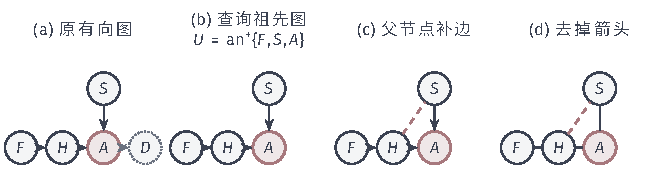
\includegraphics[width=156.951mm]{figures/06-probabilistic-graphical-models/01-representation/tikz/pgm-representations-ancestral-moralization/figure.pdf}
  \caption{报警查询的祖先道德图构造。原图以点线表示后代$D$及边$A\to D$。检验$F\perp S\mid A$时，祖先闭包为$U=\{F,H,A,S\}$，因此先去掉$D$及这条边。随后将$A$的父节点$H,S$相连，虚线表示新增的$H-S$边；再去掉原箭头，得到祖先道德图。红色的$A$是给定节点，检测分离时将其删除。}
  \label{fig:pgm-representations-ancestral-moralization}
\end{figure*}

图~\ref{fig:pgm-representations-ancestral-moralization}依次展示原有向图、查询祖先图、父节点补边和去箭头。点线标出随后筛除的后代，$H-S$虚线记录报警因子涉及的两个父节点。删除条件节点$A$后，路径$F-H-S$仍然连接，因此图不能推出$F\perp S\mid A$。若查询不包含$A$及其后代，祖先集合及由它产生的补边都可能不同。

\subsection{弦化与完美消元序}
\label{sec:pgm-representations-chordal-conversion}

推断时常常要逐个消去变量：第~\ref{chap:pgm-elimination}章会看到，消去$x_i$的标准做法是先把所有涉及$x_i$的局部因子相乘，再对$x_i$的各个状态求和。相乘后的新因子通常同时依赖$x_i$的若干个尚未删除的邻居；要让这个新作用域在无向图上仍是一个合法的团，这些邻居之间最好本来就有边。若它们缺边，就临时补一条边把作用域记录下来，这条边称为填充边；它也为无向表示改写成有向表示提供所需邻域结构。

图中不再有长度至少为四的诱导环时，就得到弦图。
给定节点顺序，本章将剩余邻域记为$N_k^+=\{v_\ell:\ell>k,\{v_k,v_\ell\}\in E\}$。
每个$N_k^+$中的剩余邻居都两两相连时，该顺序称为完美消元序；消元沿此顺序无需补边，边沿反序定向后，各节点的父节点也两两相连，形成完美有向图。

有限无向图存在完美消元序，当且仅当它是弦图。图~\ref{fig:pgm-representations-chordal-conversion}为四环加入$1-3$后，可按$(4,2,1,3)$消元：删除$4$或$2$时，剩余邻居$1,3$已由填充边相连；再删除$1$与$3$时，至多剩一个邻居，邻居两两相连的条件自动满足。将每条边从序中较晚的节点指向较早的节点，就得到无环且父集成团的有向图。定向采用消元次序的反序，因为当前节点的父节点正是尚未消去的邻居。

\begin{figure}[htbp]
  \centering
  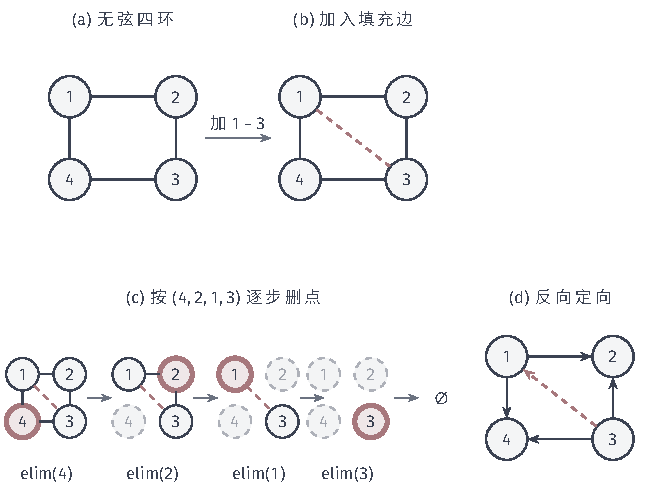
\includegraphics[width=112.000mm]{figures/06-probabilistic-graphical-models/01-representation/tikz/pgm-representations-chordal-conversion/figure.pdf}
  \caption{四环弦化及反序定向。加入虚线边$1-3$后，按完美消元序$(4,2,1,3)$删点；红色双圈为当前节点，灰色虚线轮廓为已删节点。各步下方的$\operatorname{elim}$标签记录被删除的节点，每一步的剩余邻居都两两相连。最后从序中较晚节点指向较早节点，实线箭头对应原四环的边，虚线箭头对应填充边。}
  \label{fig:pgm-representations-chordal-conversion}
\end{figure}

\Needspace{6\baselineskip}
\section{有向图与无向图的条件独立性关系}
\label{sec:pgm-representations-independence}

比较转换前后的独立性，需要精确描述两个集合：一个具体分布$p$实际满足的条件独立关系，以及一张图$\mathcal{G}$通过分离规则声明的条件独立关系。前者可能包含特殊参数造成的独立，后者则是结构对整类分布的保证。转换前后比较的，正是这两个集合之间的包含方向。下面先把它们写成集合，再定义三种刻画图与分布吻合程度的映射。

\subsection{独立性映射}
\label{sec:pgm-representations-maps}

将分布$p$的所有条件独立关系记为$\mathcal{I}(p)$：
\begin{equation}
  \mathcal{I}(p)
  =
  \bigl\{(A,B\mid S):
  \bm{X}_A\perp\bm{X}_B\mid\bm{X}_S\bigr\},
  \label{eq:pgm-representations-distribution-independences}
\end{equation}
查询集合$A,B,S\subseteq V$两两不交，$A,B$非空，条件集$S$允许为空。图的规则所蕴含的同类查询组成$\mathcal{I}(\mathcal{G})$：有向图按d-分离确定，无向图按无向分离确定。每项独立性按条件变量的分布成立；只在某个特殊条件值下成立的等式，未必属于这个集合。

这两个集合的包含方向决定图与分布的关系。图声明的独立越少，越不容易把本该相关的变量误判为独立；图声明的独立越多，对分布独立结构的限制越强。若图声明的关系全都属于分布的真实独立性，则称图为\term{独立性映射}（independency map, I-map）：图给出的每条独立保证都在分布中成立，但图可以只表达部分真实关系。若分布的全部独立性都能从图上读出，则称图为\term{依赖性映射}（dependency map, D-map）：图没有遗漏分布的任何独立，图上未被分离的变量在分布中也不独立。两个集合相等时，两项要求同时成立，图恰好刻画分布的全部独立结构，称为\term{完美映射}（perfect map）。

\begin{definition}[三类独立性映射]
  \label{def:pgm-representations-maps}
  对同一组随机变量的分布$p$与图$\mathcal{G}$，有
  \begin{equation}
    \begin{aligned}
      \mathcal{G}\text{是}p\text{的I-map}
      &\iff \mathcal{I}(\mathcal{G})\subseteq\mathcal{I}(p),\\
      \mathcal{G}\text{是}p\text{的D-map}
      &\iff \mathcal{I}(p)\subseteq\mathcal{I}(\mathcal{G}),\\
      \mathcal{G}\text{是}p\text{的完美映射}
      &\iff \mathcal{I}(\mathcal{G})=\mathcal{I}(p).
    \end{aligned}
    \label{eq:pgm-representations-map-inclusions}
  \end{equation}
\end{definition}

有向模型的可靠性保证$\mathcal{G}$是$p$的I-map；忠实性的反向蕴含再要求D-map方向成立，使有向图$\mathcal{G}$成为$p$的完美映射。这里的忠实性要求分布中的条件独立都能由图的d-分离解释，它用于排除特殊参数产生的额外独立性；其在关系识别中的作用可参考\BookChapterRef{chap:causal-inference}{卷2《数学准备：概率、因果与决策》中“因果响应”章}。

完全无向图与无边图提供了两个包含关系的极端。完全图没有分离任何两个非空节点集，因此没有独立性声明，对任意$p$都是I-map。无边图则声明所有互不相交的变量组在给定其他不交变量后独立，它的声明集包含任意$p$的真实关系，故总是D-map，通常却不是$p$的I-map。D-map的“依赖”可从逆否关系理解：对给定的$A,B,S$，图没有用$S$分离$A,B$时，$\bm{X}_A$与$\bm{X}_B$在$p$中给定$\bm{X}_S$也不独立。该保证覆盖全部查询。建模通常先满足I-map要求，因为任何错误的独立性约束都会将目标分布$p$排除在模型类之外\scite{pgm-koller2009}。

任何完全图都是I-map，但它一条独立都不声明，作为模型过于臃肿。建模时通常在保证I-map（不产生错误独立）的前提下尽量删边，因为边越少、因子越小、推断越省。若一张I-map的任一边被删后都会产生分布并不满足的错误声明，就称为\term{最小I-map}（minimal I-map）：再删任何一条边都会破坏安全性。这种最小性只针对当前图的单边删除，既不决定全体候选图中的最少边数，也不决定唯一图。例如两个二元变量取
\[
  p(0,0)=p(1,1)=0.4,\qquad
  p(0,1)=p(1,0)=0.1.
\]
两边缘都满足$p(X_1=0)=p(X_2=0)=0.5$，但$p(0,0)\ne0.25$，所以两变量依赖。$X_1\to X_2$与$X_1\leftarrow X_2$都没有额外独立声明；删边则会要求两变量独立，因此两图都是最小I-map。由此可见，单边删除的最小性保留了依赖，却无法确定方向。在一般图中，这种最小性还可能与遗漏其他真实独立性同时出现。

比较两张图时也可用同一包含方向：若$\mathcal{I}(\mathcal{G}_2)\subseteq\mathcal{I}(\mathcal{G}_1)$，称$\mathcal{G}_2$为$\mathcal{G}_1$的I-map。$\mathcal{G}_2$的独立性约束较少，仅受这些Markov约束、没有额外参数限制的分布族就较大。道德化与添加填充边通常给出这类较弱的独立性描述。

\subsection{d-分离的无向判据}
\label{sec:pgm-representations-ancestral-moralization}

第~\ref{sec:pgm-representations-ancestral-graphs}节构造的祖先道德图不只是示意，它恰好给出一个可操作的判据：d-分离不必再逐条路径分辨碰撞点，而可以完全转成无向图上的“删节点看连通”。选取查询祖先后，保留节点中的每个条件因子都只涉及这些节点；道德化再将其共同父节点相连。对所得无向图检查分离，可以精确回答原有向图的d-分离查询。

对有限DAG中两两不交的$A,B,S$，其中$A,B$非空，先取$U=\operatorname{an}^{+}(A\cup B\cup S)$，再在诱导图$\mathcal G[U]$上道德化。此时删去$S$后的无向分离，与原图中给定$S$的d-分离等价。这个等价关系只涉及图；后文将结合函数分解，证明分离查询所要求的概率独立性。

该判据在图上成立，因而与条件表参数及分布正性无关。检测按祖先闭包、诱导子图、道德化、删除条件节点$S$的次序进行：一个已观测的碰撞点在最后一步被删去，它的两个父节点之间的补边却应保留。先删除碰撞点会漏掉这条边，改变查询结果。Lauritzen的教材系统讨论祖先道德图与全局Markov性质\scite{pgm-lauritzen1996}。

对图~\ref{fig:pgm-representations-ancestral-moralization}中的$F\perp S\mid A$查询，最后删去$A$后，新增的$H-S$边仍留下路径$F-H-S$，所以当前图没有条件独立的保证。检验$F\perp S$时，祖先集合只有$\{F,S\}$，其余$H,A,D$都被去掉，剩余无边图给出独立性。同一原图的两个查询因此使用不同的祖先图，补边随$(A,B\mid S)$变化；未分离的查询仍可能在特殊参数下独立。

祖先闭包既保留端点，也保留导致间接联系的节点。例如$X_1\leftarrow X_0\to X_2$中，查询$X_1\perp X_2$需要$X_0$这个共同祖先；若仅留下$\{1,2\}$，两节点之间的联系会被误删。观测节点的祖先也有作用：在$X_1\to X_3\leftarrow X_2$、$X_3\to X_4$中，给定$X_4$激活了$X_3$处的碰撞点。查询$\{1\}$与$\{2\}$给定$\{4\}$时，祖先图保留$X_3$，随后道德化生成$1-2$边，记录这条被激活的联系。

若改为一次性道德化整个报警模型，新增边在所有查询中都保留。即使没有给定$A$，路径$F-H-S$也存在，原来的$F\perp S$就无法从整张道德图读出。\emph{整个有向图的道德图}用于重组联合函数的全部作用域，\emph{为查询构造的祖先道德图}则用于精确回答某项分离；整体图通常声明的独立性更少，其关系为
\begin{equation}
  \mathcal{I}\bigl(\operatorname{mor}(\mathcal{G})\bigr)
  \subseteq \mathcal{I}(\mathcal{G}),
  \label{eq:pgm-representations-moral-inclusion}
\end{equation}
整体图中被$S$分离的两侧，在较小的查询祖先道德图中仍被分离，所以整体图能证明部分d-分离。整体图中连通时，查询祖先图却可能已删除造成连通的节点或补边，因此原有向图仍可能满足这项d-分离。

\subsection{有向图独立性结论的证明}
\label{sec:pgm-representations-directed-proofs}

本节集中补全第~\ref{chap:pgm-directed}章引用但未展开的几个证明，第一次阅读时若主要关心结论与转换方法，也可以先跳过本节、直接进入第~\ref{sec:pgm-representations-factorizations}节的因子分解比较。证明的主线是：先用祖先道德图让局部因子的作用域全部落成团，从而把第~\ref{chap:pgm-undirected}章“分离后两侧分别归一化”的技巧搬到有向图上；再据此依次证明d-分离的可靠性、有向Markov毯以及模型类完备性。下面先说明局部条件分布如何归一化并产生联合分解，作为后续证明的共同基础。

\begin{proof}[引理~\ref{lem:pgm-directed-normalization}的证明]
取拓扑序中最后的节点，它没有子节点，只出现在自己的局部条件因子内。对其取值关于$\mu_i$积分，该因子由局部归一化变成$1$。继续逆拓扑序消去剩余节点，非负性允许用Tonelli定理交换积分次序，最后整个乘积的积分为$1$。有限离散状态下，同一操作就是逐节点求和。

求祖先集合的边缘分布时，仅需消去$V\setminus W$。集合$W$包含各节点的全部祖先，故$V\setminus W$中的节点没有位于$W$的子节点。逆拓扑序处理补集时，当前节点在补集中的子节点也已被消去，所以它仍只出现在自己的因子中。每次积分都将此因子变为一，最终留下式~\eqref{eq:pgm-directed-ancestral-marginal}中祖先节点的因子。
\end{proof}

\begin{proof}[定理~\ref{thm:pgm-directed-ordered-factor}的证明]
使用有序Markov假设指定的拓扑序，将联合概率按链式法则展开：
\[
  p(x_1,\ldots,x_d)=
  \prod_{i=1}^{d}p(x_i\mid x_1,\ldots,x_{i-1}).
\]
父节点都在当前节点之前。式~\eqref{eq:pgm-directed-ordered}使每个节点的条件分布只需保留前驱中的父节点变量：
\[
  p(x_i\mid\bm{x}_{\operatorname{pre}(i)})
    =p(x_i\mid\bm{x}_{\operatorname{pa}(i)}).
\]
代回链式法则，就得到式~\eqref{eq:pgm-directed-factorization}的父子分解。条件等式按前驱配置的分布几乎处处成立，因此还需说明零概率配置不会破坏乘积相等。

在有限离散情形，将按父配置选定的条件表记为$q_i$。父配置具有正概率时，$q_i$就是原分布的相应条件概率；父配置概率为零时，才可任选一行归一化概率来补全。完整前驱配置为零，未必意味着它包含的父配置也为零，所以不能据此前缀任意改变一行已经确定的父条件表。链式条件分布在零概率前驱上的版本可任意选择，与父条件表的补全范围需要分开。

记原分布前$k$个变量的边缘质量函数为$p_k$，并定义局部乘积
\[
  \widehat p_k(x_1,\ldots,x_k)
    =\prod_{i=1}^k q_i(x_i\mid\bm{x}_{\operatorname{pa}(i)}),
  \qquad \widehat p_0=p_0=1.
\]
我们按前缀长度证明$\widehat p_k=p_k$。若某个前缀满足$p_k(x_1,\ldots,x_k)>0$，下一节点的父配置也有正概率。有序Markov性质便将该前缀下的链式条件概率约简为已选定的$q_{k+1}$，因而
\[
  \begin{aligned}
    \widehat p_{k+1}
      &=\widehat p_k\,q_{k+1}
       =p_k\,p(x_{k+1}\mid x_1,\ldots,x_k)\\
      &=p_{k+1}.
  \end{aligned}
\]
若旧前缀的概率为零，归纳假设给出$\widehat p_k=0$，乘上下一张合法条件表后仍为零；原分布中任一延长前缀的概率也不超过旧前缀概率，所以$p_{k+1}=0$。这一步不改变正概率父配置上的条件表，也允许在零概率父配置上采用先前任意补全的行。两种情况覆盖全部前缀，从而在$k=d$得到所需联合分解。

连续密度则使用相应条件版本和积分的链式法则，得到几乎处处相同的联合密度。某个点的密度为零并不等同于离散前缀事件的概率为零，所以上面的逐配置归纳只用于有限离散情形。这一展开及约简都沿最初指定的同一拓扑序进行。
\end{proof}

\begin{proof}[定理~\ref{thm:pgm-directed-factor-local}的证明]
固定节点$i$，取非后代集合$N=\operatorname{nd}(i)$。其中各节点的祖先都仍在$N$中：若祖先是$i$或其后代，该节点就会成为$i$的后代；而$i$本身的祖先也在$N$内。因此，$N$与$N\cup\{i\}$都是祖先闭合集合，可以用引理~\ref{lem:pgm-directed-normalization}边缘化：
\[
  \begin{aligned}
    p(x_i,\bm{x}_N)
      &=q_i(x_i\mid\bm{x}_{\operatorname{pa}(i)})
        \prod_{j\in N}q_j(x_j\mid\bm{x}_{\operatorname{pa}(j)})\\
      &=q_i(x_i\mid\bm{x}_{\operatorname{pa}(i)})p(\bm{x}_N).
  \end{aligned}
\]
在有效条件值上约去非后代的边缘分布，得到$p(x_i\mid\bm{x}_N)=q_i(x_i\mid\bm{x}_{\operatorname{pa}(i)})$。再消去$N\setminus\operatorname{pa}(i)$，可见$q_i$也给出$p(x_i\mid\bm{x}_{\operatorname{pa}(i)})$的一个版本。给定父节点后，其他非后代不再改变节点的条件分布，局部Markov性质因而成立。

任一固定拓扑序都满足$\operatorname{pre}(i)\subseteq N$。在刚得到的局部独立关系中消去其余非后代，就获得该顺序下的有序Markov性质。由此，一个父子分解先推出局部性质，再推出所有拓扑序的有序性质。
\end{proof}

全局证明将查询祖先图内的因子分为两组。下面以离散求和书写；连续变量具有联合密度时，使用相应基准测度的积分，非负性使Tonelli定理适用。

\begin{proof}[定理~\ref{thm:pgm-directed-soundness}的证明]
取$p\in\mathcal{M}(\mathcal{G})$，并设查询满足$A\perp_{\mathcal{G}}B\mid S$。定理~\ref{thm:pgm-directed-ordered-factor}将$p$写成$\mathcal{G}$上的条件因子乘积，以$q_i(x_i\mid\bm{x}_{\operatorname{pa}(i)})$记节点$i$的因子。取查询祖先集合$R=\operatorname{an}^{+}(A\cup B\cup S)$，由引理~\ref{lem:pgm-directed-normalization}消去$V\setminus R$，留下
\[
  p(\bm{x}_R)=
  \prod_{i\in R}q_i(x_i\mid\bm{x}_{\operatorname{pa}(i)}).
\]
每个因子的作用域$\{i\}\cup\operatorname{pa}(i)$都在$\operatorname{mor}(\mathcal{G}[R])$中构成团。因此，删去$S$后，同一个因子剩余的节点都在同一连通分量中；两两相连的节点无法分属不同分量。

在$\operatorname{mor}(\mathcal{G}[R])\setminus S$中，将与$A$相交的分量合为$C$，其他节点合为$D=R\setminus(C\cup S)$。祖先道德化判据保证$B\subseteq D$。将涉及$C$的因子相乘记为$g(\bm{x}_C,\bm{x}_S)$，涉及$D$的因子相乘记为$h(\bm{x}_D,\bm{x}_S)$，其余只涉及$S$的因子相乘记为$k(\bm{x}_S)$，得到
\[
  p(\bm{x}_R)=
  g(\bm{x}_C,\bm{x}_S)
  h(\bm{x}_D,\bm{x}_S)
  k(\bm{x}_S).
\]
将未查询的$C\setminus A$和$D\setminus B$变量分别从两侧消去，所得函数记为$g_A,h_B$。乘积因此仍分为查询的两侧：
\[
  p(\bm{x}_A,\bm{x}_B,\bm{x}_S)=
  g_A(\bm{x}_A,\bm{x}_S)
  h_B(\bm{x}_B,\bm{x}_S)
  k(\bm{x}_S).
\]
固定具有正且有限边缘质量或密度的$\bm{x}_S$，将两侧总权重分别记为$G(\bm{x}_S)=\sum_{\bm{x}_A}g_A(\bm{x}_A,\bm{x}_S)$和$H(\bm{x}_S)=\sum_{\bm{x}_B}h_B(\bm{x}_B,\bm{x}_S)$。归一化条件联合分布时，这两个常数各自归一化一侧函数：
\[
  \begin{aligned}
    p(\bm{x}_A,\bm{x}_B\mid\bm{x}_S)
      &=\frac{g_A(\bm{x}_A,\bm{x}_S)}{G(\bm{x}_S)}
        \frac{h_B(\bm{x}_B,\bm{x}_S)}{H(\bm{x}_S)}\\
      &=p(\bm{x}_A\mid\bm{x}_S)
        p(\bm{x}_B\mid\bm{x}_S).
  \end{aligned}
\]
上述比值使用正概率条件事件或几乎处处的有效条件密度。两侧条件边缘相乘，便得到目标条件独立性。函数可以在部分联合配置取零，这个证明仍然成立。
\end{proof}

\begin{proof}[定理~\ref{thm:pgm-directed-markov-blanket}的证明]
以$O=V\setminus(\{i\}\cup\operatorname{mb}(i))$表示毯外节点。$O=\varnothing$时，独立侧为空，结论平凡成立。取$O\neq\varnothing$，考察从$i$到$O$中任一节点的路径。它的首步必经父节点或子节点，两类节点都在$\operatorname{mb}(i)$中。

首步经过父节点$j\to i$时，$j$在路径上有一个箭尾，是非碰撞点；它又满足$j\in\operatorname{mb}(i)$，所以被观测后阻断路径。首步经$i\to j$再沿$j\to k$离开时，子节点$j$同样是已观测的非碰撞点。若路径以$i\to j\leftarrow k$开始，$j$是已观测的碰撞点，但$k$是子节点的另一个父节点，也在$\operatorname{mb}(i)$内。此时$k$仍不是路径终点，且$k\to j$的箭尾使它成为已观测的非碰撞点，路径转而在这里被阻断。

三种首段覆盖了从$i$到$O$的所有路径，每条都被$\operatorname{mb}(i)$阻断，故$i\perp_{\mathcal G}O\mid\operatorname{mb}(i)$。应用定理~\ref{thm:pgm-directed-soundness}的可靠性，得到节点与毯外变量的条件独立。

在有效条件分布上，局部函数也给出同一屏蔽关系。按定理~\ref{thm:pgm-directed-ordered-factor}分解联合概率，给定其余变量后，只有节点$i$及其子节点的因子仍含$x_i$：
\begin{equation}
  \begin{aligned}
    p(x_i\mid\bm{x}_{V\setminus\{i\}})
      &\propto q_i(x_i\mid\bm{x}_{\operatorname{pa}(i)})\\
      &\quad{}\times
      \prod_{j\in\operatorname{ch}(i)}
        q_j(x_j\mid\bm{x}_{\operatorname{pa}(j)}).
  \end{aligned}
  \label{eq:pgm-directed-blanket-conditional}
\end{equation}
右侧的其他自变量全在$\operatorname{mb}(i)$中，因而对$x_i$归一化后，条件分布仍只使用毯内变量。这里的比例式用于条件分布有定义的配置；零概率条件配置采用第~\ref{chap:pgm-directed}章说明的条件分布版本。
\end{proof}

上述结果连起了第~\ref{chap:pgm-directed}章的四种表述：定理~\ref{thm:pgm-directed-ordered-factor}由有序Markov性质得到因子分解，定理~\ref{thm:pgm-directed-soundness}再由分解得到全局性质，引理~\ref{lem:pgm-representations-global-to-local}由全局得到局部，最后定理~\ref{thm:pgm-directed-factor-local}的边缘化论证由局部得到任一拓扑序的有序性质。于是式~\eqref{eq:pgm-directed-equivalence}的等价关系成立；各步都允许联合分布在某些配置取零。

可靠性只回答了“被d-分离的一定独立”，完备性还要回答相反的一面：没有被d-分离的查询，模型类中是否真的存在一个分布让两端相关？若不存在，d-分离规则就漏报了某些结构强制的独立。完备性证明通过构造“依赖见证”分布完成。最简单的连续情形只含一个碰撞点（或其后代被观测），可用高斯条件协方差直接算出非零依赖；一般图含多个碰撞点、多条路径时，不同路径的数值作用可能相互抵消，需要随后的非平凡性引理统一处理。对于图$X\to Z\leftarrow Y$及$Z\to D$，定义
\[
  \begin{aligned}
    X&=\varepsilon_X,& Y&=\varepsilon_Y,\\
    Z&=X+Y+\varepsilon_Z,& D&=Z+\varepsilon_D,
  \end{aligned}
\]
四个噪声相互独立，均取$\mathcal{N}(0,1)$分布。独立根节点使$X,Y$边缘独立，整个系统满足上述有向分解。噪声方差相加得到$\operatorname{Var}(Z)=3$，而$D=Z+\varepsilon_D$再增加一项独立噪声，所以$\operatorname{Var}(D)=4$。两个根变量与$Z$的协方差均为$1$；与$D$的协方差也均为$1$，因为新增噪声与根变量独立。观测碰撞点或其后代后，可用这些量和高斯条件协方差公式直接计算两根节点的关系：
\[
  \begin{aligned}
    \operatorname{Cov}(X,Y\mid Z)
      &=0-\frac{1\cdot1}{3}=-\frac13,\\
    \operatorname{Cov}(X,Y\mid D)
      &=0-\frac{1\cdot1}{4}=-\frac14.
  \end{aligned}
\]
条件协方差可由回归残差得到：分别将两个根变量对观测作线性回归，再计算残差的协方差。例如观测$Z$时，两个回归系数均为$1/3$，残差为$X-Z/3$与$Y-Z/3$，其协方差是$0-1/3-1/3+3/9=-1/3$；观测$D$时同理将系数换为$1/4$。联合高斯的残差与观测独立，因而该值就是条件协方差。上面两个非零结果分别给出观测碰撞点及其后代后的依赖；要覆盖一般有向图的所有活跃路径，还需要下一步的非平凡性结果。

一般图的活跃路径可含多个碰撞点，通向条件节点的路径也可能交会。不同路径的数值作用可能抵消，因此非零边系数本身不足以提供依赖见证。图~\ref{fig:pgm-directed-cancellation}展示一个明确的抵消参数：
\[
  X=\varepsilon_X,\qquad
  Z=X+\varepsilon_Z,\qquad
  Y=-X+Z+\varepsilon_Y,
\]
噪声仍相互独立且服从$\mathcal N(0,1)$。代入中间变量后得到$Y=\varepsilon_Z+\varepsilon_Y$，故$X\perp Y$：三个边系数虽然非零，直接与间接路径上的作用却恰好相消。若将$X\to Y$的系数改为$-1+\delta$，就有$\operatorname{Cov}(X,Y)=\delta$。当$\delta\ne0$时，这项额外独立性消失。

\begin{figure}[htbp]
  \centering
  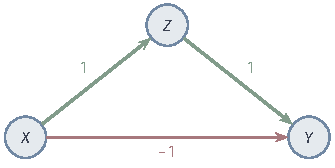
\includegraphics[width=56.653mm]{figures/06-probabilistic-graphical-models/01-representation/tikz/pgm-directed-cancellation/figure.pdf}
  \caption{直接与间接作用相消的高斯模型。$X\to Y$的系数为$-1$，经$Z$的两个系数均为$1$，代入后两项相消。两条路径对空条件集都活跃，这组参数却使$X$与$Y$独立。}
  \label{fig:pgm-directed-cancellation}
\end{figure}

完备性需要证明，对每项活跃查询，其条件独立约束并未在整个相容参数空间中恒成立。为检验这一点，先将条件独立写为一个等式，再将等式改写成模型参数的多项式取零。这样，图上的依赖见证问题就转成了参数空间中能否找到违反该等式的点。

高斯情形可以沿用刚才的条件协方差判据。记全体变量的协方差矩阵为$\bm\Sigma$；在非退化联合高斯模型中，两个标量条件独立，等价于它们的条件协方差为零。计算这个条件协方差需要对条件变量的协方差块$\bm\Sigma_{S,S}$求逆；乘以正的$\det(\bm\Sigma_{S,S})$后，可将逆矩阵带来的分母消去。所得量正是行指标为$(u,S)$、列指标为$(v,S)$的交叉子式，后面的分块行列式计算会给出这一关系。因此，这个子式取零等价于对应的标量条件协方差取零。

离散情形在$p(\bm x_S)>0$的配置上，将条件独立等式两侧的条件概率换成联合概率比值，再交叉相乘，得到下面的两项概率乘积之差。若$p(\bm x_S)=0$，相关联合质量也都为零，交乘式自动成立，无需在零概率事件上取比值。联合概率是有限个条件表项的乘积，边缘概率又是联合概率的有限和，所以该差也是条件表自由参数的多项式。

这里的“非零多项式”表示它不恒等于零，允许在特殊参数处取零；抵消例正是这样的特殊取值。下面的引理将活跃路径的图论条件转为多项式不恒为零的保证，之后的代数步骤由此选择一个违反独立约束的参数。离散结论及路径构造采用Meek的强完备性结果，高斯结论采用线性高斯有向图的多项式完备性结果\scite{pgm-directed-meek1995,pgm-koller2009}。

\begin{lemma}[条件独立约束的非平凡性]
  \label{lem:pgm-directed-nontrivial}
  设$\mathcal{G}=(V,E)$为有限有向无环图，$u,v\in V$为不同节点，$S\subseteq V\setminus\{u,v\}$，且$u,v$在$\mathcal{G}$中给定$S$时d-连接，则以下两项成立。
  \begin{enumerate}
    \item 对$i\in V$，在线性高斯系统
    \[
      X_i=\sum_{j\in\operatorname{pa}(i)}b_{i,j}X_j+\varepsilon_i,
      \qquad
      \varepsilon_1,\ldots,\varepsilon_d
      \mathrel{\overset{\mathrm{ind}}{\sim}}\mathcal N(0,1)
    \]
    中，记边系数为$\bm{\theta}$、协方差矩阵为$\bm{\Sigma}(\bm{\theta})$，则
    \[
      f_{u,v,S}(\bm{\theta})
      =\det\bm{\Sigma}_{(u,S),(v,S)}(\bm{\theta})
    \]
    是非零多项式。行指标按$u$及$S$排列，列指标按$v$及同一顺序的$S$排列；$S=\varnothing$时，该式为$\Sigma_{u,v}$。
    \item 固定每个节点至少含两个状态的有限状态空间，并用各行前$r_i-1$个概率参数化局部条件表。将联合概率与边缘概率写成这些参数的多项式后，在所有状态配置对应的条件独立多项式
    \[
      p(x_u,x_v,\bm{x}_S)p(\bm{x}_S)
      -p(x_u,\bm{x}_S)p(x_v,\bm{x}_S)
    \]
    中，至少有一个不是零多项式。
  \end{enumerate}
\end{lemma}

本章采用这一外部引理，下面的证明以它为前提。引理所处理的是活跃路径及碰撞点通向$S$的有向路径：从中提取保留连接的子图，并控制路径交会时的代数抵消。高斯模型可以使用任意正噪声方差，这里的单位方差子类已足够构造所需见证；逐坐标可逆缩放也保持条件独立性。具体地，若原噪声标准差为$\sigma_i>0$，令$Y_i=X_i/\sigma_i$，新噪声就具有单位方差，边系数则变为$b_{i,j}\sigma_j/\sigma_i$。这种缩放没有丢掉任何坐标信息，所以不会改变条件独立关系。

\begin{proof}[定理~\ref{thm:pgm-directed-completeness}的线性高斯部分]
集合$A,B$未被$S$ d-分离时，可选由活跃路径连接的$u\in A,v\in B$。将引理~\ref{lem:pgm-directed-nontrivial}的线性系统按拓扑序写为矩阵形式，得到$\bm X=\bm B\bm X+\bm\varepsilon$；系数矩阵$\bm{B}$严格下三角，非边元素为零。于是$\bm X=(\bm I-\bm B)^{-1}\bm\varepsilon$，再利用$\bm{B}^d=\bm 0$，得到
\[
  \begin{aligned}
    \bm{L}&=(\bm{I}-\bm{B})^{-1}
       =\bm{I}+\bm{B}+\cdots+\bm{B}^{d-1},\\
    \bm{\Sigma}(\bm{\theta})&=\bm{L}\bm{L}^{\top}.
  \end{aligned}
\]
有限矩阵和使协方差各元素都成为边系数的多项式；对任意实边系数，可逆的线性变换又保证$\bm{\Sigma}$正定。将条件协方差写入分块行列式，可得
\[
  f_{u,v,S}(\bm{\theta})
    =\det(\bm{\Sigma}_{S,S})
      \bigl(\Sigma_{u,v}
        -\bm{\Sigma}_{u,S}\bm{\Sigma}_{S,S}^{-1}
         \bm{\Sigma}_{S,v}\bigr).
\]
括号给出$\operatorname{Cov}(X_u,X_v\mid\bm X_S)$。$S$为空时，空矩阵行列式取$1$，矩阵求逆项无需执行。高斯条件分布的两个标量独立当且仅当这个协方差为零。引理保证$f_{u,v,S}$为非零多项式，所以可以选取使条件协方差非零的系数。

存在性还可落实为有限终止的枚举：逐渐增大有理数分子绝对值及正分母的上界，枚举有理边系数向量，用有理数运算计算行列式，找到非零值即停止。非零多项式在某个实参数点附近仍非零，有理向量的稠密性保证枚举能进入这个邻域。输出系数与单位独立高斯噪声定义了$\mathcal{M}_{\mathrm{LG}}(\mathcal{G})$中的分布，满足$X_u\not\perp X_v\mid\bm X_S$。若向量$\bm X_A,\bm X_B$条件独立，每对分量也应条件独立，因而与上述结果矛盾。这给出了查询的见证构造，但并未给出高效寻找见证的算法。
\end{proof}

有限离散模型改用条件表参数。每一行取前若干状态概率为自由参数，末状态概率由行和为$1$确定。各自由坐标大于$0$且每行自由坐标之和小于$1$，恰好保证整行严格为正。这些都是严格不等式，多行参数的笛卡尔积因而在有限维参数空间中形成开集；每行均匀分布给出其中一个点，说明该开集非空。联合概率与边缘概率都是这些参数的多项式。严格正性保证$p(\bm x_S)>0$，所以给定$S$时$X_u$与$X_v$条件独立，等价于每种状态配置都满足
\[
  \begin{aligned}
    &p(x_u,x_v,\bm x_S)p(\bm x_S)\\
    &\qquad{}-p(x_u,\bm x_S)p(x_v,\bm x_S)=0.
  \end{aligned}
\]

要从不恒为零走到这个严格正参数域内的见证，还需知道：非零多项式的零点不可能占满一个非空开集。下面用零点集的测度说明这一事实，也为随后同时避开多项额外独立约束作准备。

\begin{lemma}[非零多项式的零点集]
  \label{lem:pgm-representations-polynomial-zero-set}
  设$f$是$\mathbb R^m$上不恒为零的实多项式，$m\geq1$。其零点集具有$m$维Lebesgue测度零，因此不能包含非空开集。
\end{lemma}

\begin{proof}
记$\lambda_m$为$m$维Lebesgue测度。$m=1$时，非零多项式只有有限个实根，故零点集的测度为零。设结论对$m-1$个变量成立，将$m$元多项式按最后一个坐标$t$展开为
\[
  f(\bm y,t)=\sum_{\ell=0}^{K}a_\ell(\bm y)t^\ell,
  \qquad \bm y\in\mathbb R^{m-1}.
\]
至少有一个系数多项式$a_{\ell_0}$不恒为零。使所有系数同时为零的底点集合记为$E$，它包含在$a_{\ell_0}$的零点集中，因归纳假设而有$\lambda_{m-1}(E)=0$。在$E$之外，每个固定$\bm y$对应一元非零多项式，它的零点只有有限个，故沿$t$方向的截面测度为零。

先将零点集限制在盒$[-M,M]^m$内，其中$M$为正整数。在坏底点$E$上，截面长度至多为$2M$；在其余底点上，截面长度为零。零点集是闭集，可以对其非负指标函数使用Tonelli定理，按底点与最后一个坐标分别积分。积分只可能在零测的$E$上贡献至多$2M$，所以整个盒内零点集的$m$维测度仍为零。再令$M=1,2,\ldots$，这些盒覆盖全空间，可数个零测集的并仍为零测集。任一非空开集含有边长为正的小盒，具有正测度，因此不能包含在该零点集中。
\end{proof}

\begin{proof}[定理~\ref{thm:pgm-directed-completeness}的有限离散部分]
取活跃路径连接的$u\in A,v\in B$。引理~\ref{lem:pgm-directed-nontrivial}的第二项保证，有限组条件独立多项式中至少一项非零。由引理~\ref{lem:pgm-representations-polynomial-zero-set}，非零多项式在参数空间的非空开集上无法恒为零。严格正条件表参数域正是这样的开集，所以其中必有一点使选定多项式非零，至少一个独立等式随之失败。所得联合分布属于$\mathcal{M}_{\mathrm{disc}}^{+}(\mathcal{G})$，并满足$X_u\not\perp X_v\mid\bm X_S$。向量$\bm X_A\perp\bm X_B\mid\bm X_S$若成立，会推出所有坐标对条件独立，与选定坐标对的结论矛盾。故$\bm X_A\not\perp\bm X_B\mid\bm X_S$，有限离散类也存在所需见证。
\end{proof}

对固定有限图，所有节点对及条件集合的查询只有有限多组。为每项未分离查询选定一个非零检验多项式：高斯情形选上述交叉子式，离散情形选引理保证不恒为零的某一状态配置等式。该查询若出现额外独立性，选定多项式就必须取零。因此，导致该查询额外独立的坏参数集包含在一个零测集中，而不要求它恰好等于整个零点集。有限个这样的零点集之并仍为零测集，无法覆盖具有非空内部的合法参数域。选取并集之外的同一组参数，就能同时避免所有节点对查询的额外独立性；任何未分离的向量查询又含有一对活跃连接的坐标，故也不可能额外独立。

这一论证也覆盖正噪声方差自由变化的线性高斯模型，而不限于构造见证所用的单位方差子类。令$\tau_i>0$为第$i$项噪声方差，协方差变为$\bm\Sigma=\bm L\operatorname{diag}(\tau_1,\ldots,\tau_d)\bm L^\top$，其元素仍是边系数和方差坐标的多项式。每个检验多项式在所有$\tau_i=1$的子类中已不恒为零，所以在更大的参数空间中也不恒为零；正方差条件给出的域仍是非空开集。截距只改变均值，不影响这些条件独立判据，把截距也列作自由坐标后仍可使用同一零点集结论。因此，在上述没有额外约束的离散或线性高斯参数族中，忠实分布存在，不忠实参数组成零测集。真实系统可能具有特殊参数；接近抵消集合时，依赖还可能很弱，使有限样本难以分辨。

\subsection{两类独立性表示的差异}
\label{sec:pgm-representations-independence-differences}

查询祖先道德图随端点和条件集合而变化；一张固定的无向图未必能同时复现所有d-分离。例如碰撞结构$X_1\to X_3\leftarrow X_2$声明$X_1\perp X_2$，没有声明$X_1\perp X_2\mid X_3$。无向图若使$1$与$2$被空集分离，两节点之间原本就无路径；再删$3$仍然分离。这个单调性与碰撞查询的变化冲突，所以同一节点集合上无法找到完全相同的无向分离集合。特殊参数产生的分布仍可由两类图共同表示，当前反例比较的是图的全部独立性声明。

从无向图转向有向图也存在表达边界。图~\ref{fig:pgm-representations-chordal-conversion}左侧四环$1-2-3-4-1$没有对角边$1-3$或$2-4$，同时声明
\begin{equation}
  X_1\perp X_3\mid(X_2,X_4),\qquad
  X_2\perp X_4\mid(X_1,X_3).
  \label{eq:pgm-representations-cycle-independences}
\end{equation}
给这个骨架作无环定向，至少一个节点会同时接收两条环边。例如$2\to1\leftarrow4$的两父节点$2$与$4$不相邻，形成未遮蔽碰撞点。给定$\{1,3\}$会打开路径$2\to1\leftarrow4$，所以d-分离无法得到式~\eqref{eq:pgm-representations-cycle-independences}的第二项。

这一碰撞点可由拓扑序直接找出：四环中排在最后的节点，其两个邻居都在前，故两条边都指向它。更换拓扑序会改变碰撞的位置，仍会留下一个未遮蔽碰撞点。

改变骨架也无法保留原来的全部独立性。对有向图中两个不相邻节点$i,j$，无环性保证可以选一个节点，例如$i$，使$j$是它的非后代。$j$又不是$i$的父节点，第~\ref{chap:pgm-directed}章证明局部Markov性质时所用的图分离关系便给出$i\perp_{\mathcal G}j\mid\operatorname{pa}(i)$。这一步只涉及图；再应用可靠性，才得到相容分布中的$X_i\perp X_j\mid\bm{X}_{\operatorname{pa}(i)}$。无向图中的非邻接对则被其余全部节点分离。相邻对在两类图中都保留长度为一的路径，任何不含端点的条件集都无法阻断它。由此，全部图分离关系能确定邻接关系，两张图独立性集合相同时也必有同一骨架。

碰撞结构的观测激活与四环的两项对角条件独立，分别超出了另一类图在同一节点集上的完美表示范围，所以两类图的独立性表达能力一般互不包含。第~\ref{sec:pgm-representations-chordal-conversion}节的弦图和完美有向图则提供了可相互保留全部分离关系的结构条件。

\subsection{完美表示的条件}
\label{sec:pgm-representations-perfect-dags}

碰撞结构和无弦四环说明两类图的独立性表达能力一般互不包含。能够无损保留全部分离关系的结构由弦图以及“父集成团”的有向图给出，二者是同一性质在两种图上的体现。以下两个判定分别用于无向到有向、有向到无向的完美表示。

对于有限无向图，要在同一节点集合上用DAG保留全部分离关系，原图必须是弦图，而弦图也允许这种改写。选取一个完美消元序，将每条边从序中较晚的节点指向较早的节点，便得到所需的完美有向图。此时原剩余邻域成为父集，每个父集中的节点两两相连。


对有限DAG，同一节点集合上的完美无向表示，要求各节点父集内的节点两两相连；这个条件也足以保证表示存在。每个父集内的节点已经两两相连时，道德化无需额外补父节点之间的边，去掉方向后的骨架就是弦图，并保留同样的分离关系。

“完美有向图”的判定只用父集是否成团；“$\mathcal{D}$是$p$的完美映射”则比较图与某个分布的独立性。即使$\mathcal{D}$和$\mathcal{U}$的分离集合完全相等，特殊参数仍可能让$p$具有额外独立性。这两种转换保证的是图之间的完美表示，具体分布的完美映射还需忠实性。

原图不满足弦性时，可以添加边后再定向。图~\ref{fig:pgm-representations-chordal-conversion}为四环补$1-3$，产生极大团$\{1,2,3\}$与$\{1,3,4\}$。以$\mathcal{U}$记原图、$\widetilde{\mathcal{U}}$记弦化图，则有
\[
  \mathcal{I}(\widetilde{\mathcal{U}})
  \subseteq \mathcal{I}(\mathcal{U}).
\]
填充边增加可用路径，因而新分离集合只能缩小。四环的$X_2\perp X_4\mid(X_1,X_3)$仍能从新图读出，$X_1\perp X_3\mid(X_2,X_4)$却因为新增对角边而失去图上的保证。弦化换来了所需的消元和定向结构，也可能减少可见的独立性。

\section{有向图与无向图的因子分解关系}
\label{sec:pgm-representations-factorizations}

前两节从结构和独立性两个层面比较了两种图，本节转向第三个层面：局部函数怎样重组，才能在换图的同时保持联合分布的每一个概率值都不变。以下固定一个给定分布$p$，说明它的条件分布与团势如何互相改写，同时区分“对这一个分布的精确改写”与“转换后那张图所允许的整类自由参数模型”。后者通常比原来的分布族更大，因为一旦不再约束新表项之间的关系，模型就能表达转换前没有的分布。两种分解在归一化方式上的差异，决定了转换时必须额外处理的内容。

\subsection{两类因子分解的差异}
\label{sec:pgm-representations-normalization}

有向图把联合分布写成每个节点给定父节点的条件分布乘积：
\begin{equation}
  p(\bm{x})=\prod_{i\in V}
  p(x_i\mid\bm{x}_{\operatorname{pa}(i)}).
  \label{eq:pgm-representations-directed-product}
\end{equation}
每个父配置下，局部条件表都满足$\sum_{x_i}p(x_i\mid\bm{x}_{\operatorname{pa}(i)})=1$。从没有子节点的节点开始求和，它只在自己的条件因子中出现，这个因子因此变成$1$。剩余图仍无环，可以继续同样的操作，最后得到$\sum_{\bm{x}}p(\bm{x})=1$。局部归一化与无环结构共同保证了联合归一化。

Markov网络使用团上的非负势，另以全局配分函数归一化：
\begin{equation}
  p(\bm{x})=\frac{1}{Z}
  \prod_{C\in\mathcal{C}}\psi_C(\bm{x}_C),
  \qquad
  Z=\sum_{\bm{x}}\prod_{C\in\mathcal{C}}\psi_C(\bm{x}_C),
  \label{eq:pgm-representations-undirected-product}
\end{equation}
所选团作用域组成$\mathcal{C}$，其中可含极大团或较小团，且需满足$0<Z<\infty$。势表给出相对权重，对单个变量的求和可以异于$1$。不同势共享坐标，逐表归一化后，整体乘积仍需自己的归一化常数。将一个势乘以正常数时，$Z$同比缩放，分布$p$保持原样；这种尺度自由度构成势参数的冗余。

连续变量改用指定乘积测度的积分，函数需可测、非负且可归一化，局部密度也以积分为一理解。已给定非负团分解时，全局Markov性质允许零配置；从独立性反推团分解，则采用上一章说明的严格正性等条件。下面的条件表重组使用有限离散严格正分布，使每步条件归一化的分母都为正。

\subsection{从有向因子分解到无向因子分解}
\label{sec:pgm-representations-directed-to-undirected}

从有向因子分解转换到无向因子分解更直接。有向条件因子$p(x_i\mid\bm{x}_{\operatorname{pa}(i)})$虽然带有“$i$条件于父节点”的方向含义，但作为普通多变量函数，它只依赖$\{i\}\cup\operatorname{pa}(i)$这一组变量，见式~\eqref{eq:pgm-representations-directed-product}。只要在无向图中把这个“家庭集合”连成一个团，就可以直接把整张条件表当成该团上的势，函数值保持不变。整体道德化恰好完成补边，使每个家庭集合都成为团，因此原条件分布可作为该团的势：
\[
  \psi_{\{i\}\cup\operatorname{pa}(i)}
  (x_i,\bm{x}_{\operatorname{pa}(i)})
  =
  p(x_i\mid\bm{x}_{\operatorname{pa}(i)}),
\]
全部势相乘仍是原来的条件分布乘积；相同作用域的因子可以保留，也可以合并。原联合分布已归一化，故此时$Z=1$。若只保留极大团势，就给每个因子选择一个包含它的极大团，在团内相乘；未接收因子的团用常数$1$。每个因子参与一次，联合函数因此不变。极大团按包含关系覆盖局部作用域，适合完成这种分配；仅选节点数最多的团，可能遗漏其他作用域。

将报警模型的四个条件或先验因子分配给两个极大团，就得到
\begin{equation}
  \begin{aligned}
    p(f,h,a,s)&=p(f)p(s)p(h\mid f)p(a\mid h,s)\\
    &=\psi_{\{F,H\}}(f,h)\,
      \psi_{\{H,A,S\}}(h,a,s),\\
    \psi_{\{F,H\}}(f,h)&=p(f)p(h\mid f),\\
    \psi_{\{H,A,S\}}(h,a,s)&=p(s)p(a\mid h,s).
  \end{aligned}
  \label{eq:pgm-representations-alarm-potentials}
\end{equation}
新增的$H-S$边让道德图容纳报警因子的三元作用域，也使图上无法读出$F\perp S$。原因子保留的分布仍有这项独立性，对$a,h$求和便可验证：
\[
  \sum_h\sum_a p(f)p(s)p(h\mid f)p(a\mid h,s)
  =p(f)p(s).
\]
两势中的条件归一化关系让该等式继续成立，而新图的路径规则没有编码这些关系。若把两势表作为自由权重任意修改，图所允许的其他分布就可能失去$F\perp S$。

用人工参数可计算报警观测后的关系变化。取$p(F=1)=0.1$、$p(S=1)=0.05$，以及$p(H=1\mid F=1)=0.8$、$p(H=1\mid F=0)=0.1$，得到$p(H=1)=0.17$。在$(h,s)=(0,0),(1,0),(0,1),(1,1)$四种配置下，令$p(A=1\mid h,s)$依次为$0.01,0.9,0.7,0.99$。这些值只用于演示模型计算。因$H$与$S$边缘独立，报警概率为
\[
  \begin{aligned}
    p(A=1)
    &=0.83\times0.95\times0.01
      +0.17\times0.95\times0.9\\
    &\quad+0.83\times0.05\times0.7
      +0.17\times0.05\times0.99\\
    &=0.1907.
  \end{aligned}
\]
观测到报警后，再给定不同的传感器状态，过热的后验概率分别为
\begin{equation}
  \begin{aligned}
    p(H=1\mid A=1,S=0)
    &=\frac{0.17\times0.9}
    {0.17\times0.9+0.83\times0.01}
    \approx0.9485,\\
    p(H=1\mid A=1,S=1)
    &=\frac{0.17\times0.99}
    {0.17\times0.99+0.83\times0.7}
    \approx0.2246.
  \end{aligned}
  \label{eq:pgm-representations-alarm-posteriors}
\end{equation}
两个后验概率不同，说明这组参数在给定碰撞点后产生了依赖。式~\eqref{eq:pgm-representations-alarm-potentials}的团势积与原有向积相同，因而得到同样的计算结果。$H-S$补边记录无向函数所需的作用域，分布中的概率关系在转换前后保持不变。

道德化让有$k$个父节点的子节点及其父节点组成$k+1$元团，父节点间至多增加$\binom{k}{2}$条边。每变量有$r$种状态时，稠密$(k+1)$元表包含$r^{k+1}$项。原来的一般条件表已使用同一家庭作用域，所以这张团表本身未必增加存储量。多个家庭叠加却可能形成更大的最大团；若将原小因子全部合成该团的一般表，就会增加需要保存的组合，并失去可利用的细分计算结构。

推断的主要开销由消元时形成的联合因子决定，输入边数只提供部分结构信息。道德图仍可能含无弦环，随后消元还需填充边。道德化完成的是原因子作用域的无向表示；寻找较低代价的消元结构，还要另外选择顺序。

\subsection{从无向因子分解到有向因子分解}
\label{sec:pgm-representations-undirected-to-directed}

反方向（从无向势恢复成一组有向条件表）更有讲究。最省事的做法是直接套用链式法则：沿任意顺序把联合分布写成每个变量给定全部前驱的条件分布乘积，但这样每个节点的父集几乎包含所有前驱，得到的是一张稠密有向图，完全丢掉了原无向图的稀疏邻接。若希望保留原邻接、让每个节点的父集只含它在消元时的剩余邻居，就必须借助弦图的完美消元序——这正是第~\ref{sec:pgm-representations-chordal-conversion}节引入弦化的原因。

具体做法是逐次消元，每消去一个变量就把它“当时涉及的全部因子”整理成一张以剩余邻居为条件的条件表。设$p$严格为正，在弦图$\mathcal{U}$上已有团分解，取完美消元序$v_1,\ldots,v_d$。逐次消元时，要保持如下作用域条件：处理$v_k$前，每个具有非空作用域的当前因子，都定义在剩余诱导图$\mathcal{U}[\{v_k,\ldots,v_d\}]$的团上；作用域为空的常数因子也保留在乘积中。初始因子满足此条件，所以第$1$步可用。

若第$k$步开始时条件成立，含$v_k$的团因子，其余坐标必是$v_k$尚未删除的邻居，属于$N_k^+$。相乘并消去$v_k$后，新的作用域仍包含在$N_k^+$中；该集合的节点在完美消元序下两两相连，所以非空的新作用域仍是下一张剩余图的团。若新作用域为空，就得到常数因子。不含$v_k$的因子保持原样，作用域条件由此逐步保持。

第$k$步将当前含$v_k$的因子收集为$\mathcal{B}_k$，相乘后只需$v_k$及$N_k^+$的取值。对$v_k$求和得到剩余邻居上的新因子，再用它归一化当前节点：
\begin{equation}
  \begin{aligned}
    b_k(x_{v_k},\bm{x}_{N_k^+})
    &=\prod_{\psi\in\mathcal{B}_k}\psi,\\
    a_k(\bm{x}_{N_k^+})
    &=\sum_{x_{v_k}}b_k(x_{v_k},\bm{x}_{N_k^+}),\\
    q_k(x_{v_k}\mid\bm{x}_{N_k^+})
    &=\frac{b_k(x_{v_k},\bm{x}_{N_k^+})}
    {a_k(\bm{x}_{N_k^+})}.
  \end{aligned}
  \label{eq:pgm-representations-bucket-normalization}
\end{equation}
函数可以实际忽略部分已列坐标。将$\mathcal{B}_k$的因子从当前乘积中移除，换入$a_k$，就将$v_k$边缘化了。当新因子有非空作用域时，它仍定义在团上，$a_k$所用的邻接关系都已存在于原弦图中。末步$N_d^+=\varnothing$，此时$a_d$是常数，无需给它指定一个非空团。

所得$q_k$还需与原联合分布的条件概率对应。消去$v_1,\ldots,v_{k-1}$后，当前乘积正比于剩余变量的联合边缘分布。给定其他剩余坐标时，$\mathcal{B}_k$之外的因子都不含$v_k$，在条件比值中可约掉。因而$q_k$正是该边缘分布中$v_k$给定所有剩余变量的条件分布，并且按式~\eqref{eq:pgm-representations-bucket-normalization}只依赖$N_k^+$。这个结果使用消元到当前步骤的全部相关因子，原来一张团势单独归一化通常不会给出同一条件表。

每步的归一化给出$b_k=q_k a_k$。将这些等式依次代回原势乘积，全部节点消去后留下的常数乘积等于$Z$，得到
\begin{equation}
  \begin{aligned}
    \prod_{C\in\mathcal{C}}\psi_C(\bm{x}_C)
    &=Z\prod_{k=1}^d q_k(x_{v_k}\mid\bm{x}_{N_k^+}),\\
    p(\bm{x})&=\prod_{k=1}^d q_k(x_{v_k}\mid\bm{x}_{N_k^+}).
  \end{aligned}
  \label{eq:pgm-representations-telescoping-product}
\end{equation}
以$N_k^+$为$v_k$的父集，便获得按完美消元序反向定向的有向图。父节点在消元时晚于当前节点，所以拓扑序是消元序的逆序。每张新条件表已归一化，而求出它们的过程包含了原分布的边缘化和全局归一化计算；这些工作随表重组一同完成\scite{pgm-koller2009}。

原图非弦时，剩余邻居可能缺边。消元通常产生同时依赖这些邻居的新因子，需要添加填充边容纳作用域；在填充后的弦图上仍可按上述方法精确转换。这个结构要求针对整类严格正团分布：同一构造要处理所有可能参数，就需要容纳相应的中间作用域。固定参数时，新因子还可能进一步分解，独立分布甚至无需这些联系，因此实际保留的边还可受函数结构影响。

对例~\ref{ex:pgm-undirected-cycle}的四节点环，可将每步消元与新条件表直接算出。四变量都取$\{0,1\}$，四条环边使用相同势：
\begin{equation}
  \psi_{\{i,j\}}(x_i,x_j)=
  \begin{cases}
    2,&x_i=x_j,\\
    1,&x_i\ne x_j.
  \end{cases}
  \label{eq:pgm-representations-cycle-potentials}
\end{equation}
先将四势相乘作为未归一化权重。按图~\ref{fig:pgm-representations-chordal-conversion}的顺序消去$4$，涉及它的两个边势产生
\begin{equation}
  \begin{aligned}
    m(x_1,x_3)
    &=\sum_{x_4}\psi_{\{1,4\}}(x_1,x_4)
    \psi_{\{3,4\}}(x_3,x_4)\\
    &=
    \begin{cases}
      5,&x_1=x_3,\\
      4,&x_1\ne x_3.
    \end{cases}
  \end{aligned}
  \label{eq:pgm-representations-cycle-message}
\end{equation}
在$x_1=x_3=0$时，求和的两项为$2\times2$与$1\times1$，合为$5$；两端不同时，各项为$2$，合为$4$。新函数$m$同时使用$1,3$，对应新增的$1-3$填充边。再消去$2$得到同样的$m(x_1,x_3)$，两函数相乘后的剩余权重为$m(x_1,x_3)^2$，故
\[
  Z=2\times5^2+2\times4^2=82.
\]

前两步的条件分布记为$q_4(x_4\mid x_1,x_3)$和$q_2(x_2\mid x_1,x_3)$，下标表示对应变量节点。各自的分子是两个关联边势的乘积，分母为$m$。当$x_1=x_3$，中间变量取同一状态的概率为$4/5$，另一状态为$1/5$；当$x_1\ne x_3$，两状态概率均为$1/2$。

消去$4$和$2$后，对剩余权重$m(x_1,x_3)^2$继续消去$1$。无论$x_3$取何值，都有
\[
  \sum_{x_1}m(x_1,x_3)^2=5^2+4^2=41,
\]
由此$q_1(x_1\mid x_3)=m(x_1,x_3)^2/41$。最后两个状态$x_3=0,1$各留下权重$41$，总和$Z=82$使$q_3(x_3)=41/82=1/2$。后两张条件表因此为
\begin{equation}
  q_3(x_3)=\frac12,\qquad
  q_1(x_1\mid x_3)=
  \begin{cases}
    25/41,&x_1=x_3,\\
    16/41,&x_1\ne x_3.
  \end{cases}
  \label{eq:pgm-representations-cycle-root-tables}
\end{equation}
根据各条件表的输入，父集分别是$\operatorname{pa}(3)=\varnothing$、$\operatorname{pa}(1)=\{3\}$及$\operatorname{pa}(2)=\operatorname{pa}(4)=\{1,3\}$，对应边$3\to1$、$1\to2$、$3\to2$、$1\to4$和$3\to4$。把四条件表相乘，两分母$m$与分子中的平方约去，得到原来的联合概率：
\[
  \begin{aligned}
    q_3q_1q_2q_4
    &=\frac12\,
      \frac{m(x_1,x_3)^2}{41}\,
      \frac{\psi_{\{1,2\}}\psi_{\{2,3\}}}{m(x_1,x_3)}\,
      \frac{\psi_{\{1,4\}}\psi_{\{3,4\}}}{m(x_1,x_3)}\\
    &=\frac{
      \psi_{\{1,2\}}\psi_{\{2,3\}}
      \psi_{\{1,4\}}\psi_{\{3,4\}}}{82}.
  \end{aligned}
\]

新图有$3\to1$，原来的$X_1\perp X_3\mid(X_2,X_4)$仍保留在所转换的分布中。固定$x_2=x_4=0$，以$x_1=0,1$为行、$x_3=0,1$为列，条件联合表为
\[
  \bigl[p(x_1,x_3\mid X_2=0,X_4=0)\bigr]
  =\frac1{25}
  \begin{pmatrix}16&4\\4&1\end{pmatrix}
  =
  \begin{pmatrix}4/5\\1/5\end{pmatrix}
  \begin{pmatrix}4/5&1/5\end{pmatrix}.
\]
任意给定$x_2,x_4$，原四势都可分别按$x_1$与$x_3$分组，所以每种条件取值都满足这项独立性。新有向图的$1$与$3$相邻，d-分离却无法声明它。任意修改各张转换后的条件表，会失去原边势分组所隐含的约束，因而可能使该独立性消失。

对这组数值，还可验证新图是最小I-map。$q_1$依赖$x_3$，$q_2$与$q_4$在一个父节点固定后，也分别依赖另一父节点：例如固定$x_3=0$，将$x_1$从$0$改为$1$，$q_2(X_2=0\mid x_1,x_3)$由$4/5$变为$1/2$。删去任一父边会将这种依赖排除，从而不再容纳当前分布。然而，图仍漏掉原环的一个条件独立查询，所以这个最小I-map并非完美映射。

保存表项的数量与可以独立改变的参数数量不同。一般离散有向模型每行归一化后，其自由参数总数为
\[
  \sum_{i\in V}(r_i-1)
  \prod_{j\in\operatorname{pa}(i)}r_j,
\]
这里$r_i$为$X_i$的状态数，每个父配置的行和为$1$，所以每行只有状态数减一的自由参数。无向势表还允许在因子间转移权重，同一分布有多组参数表示，因此总表项数也需去掉这类冗余后才得到自由度。

表~\ref{tab:pgm-representations-cycle-costs}以四环的\emph{完整严格正二元图模型族}为对象。式~\eqref{eq:pgm-representations-cycle-potentials}的固定数值只是其中一个分布。对取值$0,1$的两个变量，任意严格正边势的对数都可写成常数、两个一元项和一个乘积项之和：这四种函数足以逐一匹配二元表的四个值。将四条边的项收集起来，一元项合并，常数项由配分函数吸收，整类原环因而可写为
\[
  \log p(\bm x)
    =-\log Z(\bm a,\bm b)
      +\sum_{i=1}^{4}a_i x_i
      +\sum_{\{i,j\}\in E_{\mathrm{cyc}}}b_{i,j}x_ix_j,
\]
其中$E_{\mathrm{cyc}}=\{\{1,2\},\{2,3\},\{3,4\},\{1,4\}\}$为原四环的边集，$\bm a$与$\bm b$分别收集四个一元系数和四个边交互系数。四个$a_i$与四个$b_{i,j}$可以自由改变，有限状态空间保证每组有限系数都定义严格正分布。它们也没有进一步的线性冗余：先在全零配置取值，再分别在只有一个坐标为$1$和只有一条边的两端为$1$的配置取值，就能依次识别常数、一元系数和边交互系数。因此，这个模型族共有$8$个自由参数，与上一章的二元对数线性表示一致。填充后若各条件表自由变化，模型有$1+2+4+4=11$个自由参数。精确转换的条件表仍满足原$8$维族的约束；只有将它们作为自由表变化，才进入更大的模型族。

\begin{table}[htbp]
  \centering
  \begin{tabularx}{\linewidth}{@{}lXX@{}}
    \toprule
    比较项 & 原四环的边势表示 & 填充后DAG的自由条件表模型族 \\
    \midrule
    输入最大作用域 & $2$个变量 & $3$个变量 \\
    稠密表存储 & $4\times4=16$项 & $2+4+8+8=22$项 \\
    模型族自由度 & $8$ & $11$ \\
    归一化约束 & 全局配分函数$Z$ & 每张条件表逐行归一化 \\
    图独立性 & 式~\eqref{eq:pgm-representations-cycle-independences}的两项 & 只保留第二项 \\
    \bottomrule
  \end{tabularx}
  \caption{四环表示的作用域、存储及自由度。表项数按保存完整稠密表计，含归一化冗余；自由度已去掉冗余。新有向图族允许$11$个自由参数，而精确转换的表仍受原四环分布族的约束。}
  \label{tab:pgm-representations-cycle-costs}
\end{table}

最大团虽从二元变为三元，原环的消元本来就涉及三变量组合：消去$4$时，相乘的两个边势共有三个坐标，稠密计算通常枚举$r^3$种配置，再生成$r^2$项的新因子。填充图显式记录了这次已有的计算。若局部组合有$k$个变量、每变量$r$种状态，稠密表规模便为$r^k$，消元序决定可能出现的作用域。转换因而可以改变输入存储和图声明，也能显示原先隐含的中间运算；最优推断成本的变化还取决于可选的顺序及函数结构。

\section{因子图}
\label{sec:pgm-representations-factor-graphs}

前面几节用的图都只画变量：节点是随机变量，边表示它们之间的依赖。但要真正做推断计算，光知道“哪些变量相连”还不够，还必须知道联合分布被拆成了哪几个局部函数、每个函数读取哪些变量。问题在于，同一张变量邻接图可能对应完全不同的函数拆分：同一个三变量作用域，可以由一张三元表$f_{123}(x_1,x_2,x_3)$给出，也可以由三张二元表的乘积$f_{12}f_{23}f_{13}$给出——两者在变量图上都画出同样的三角形，但推断时前者要一次性读取三个变量、后者只需成对读取，计算量和中间结果都不同。变量图无法区分这两种输入，推断程序却恰恰需要据此收集函数、计算乘积。因子图就是为补上这层信息而引入的表示：它把局部函数本身也画成一类节点，显式保留“函数—变量”的归属，让有向条件分布和无向势都能以同一套结构进入局部计算。

\subsection{因子图的定义}
\label{sec:pgm-representations-factor-graph-definition}

同一张变量邻接图可能隐藏不同的函数分解。例如，一个三变量因子$f_{123}(x_1,x_2,x_3)$与三个二变量因子的乘积$f_{12}f_{23}f_{13}$都会在无向表示中连接三个变量，却需要不同的局部计算：前者要同时读取三个输入，后者分别读取三对输入。为了保留这种差别，可以把局部函数本身也画成节点，再连接它实际使用的变量。将待计算函数的局部分解写为
\begin{equation}
  g(\bm{x})=\prod_{\alpha\in\mathcal{F}}
  f_\alpha(\bm{x}_{D_\alpha}),
  \qquad D_\alpha\subseteq V.
  \label{eq:pgm-representations-factor-graph-product}
\end{equation}
因子以$\mathcal{F}$为索引，函数$f_\alpha$需要输入的变量集为$D_\alpha$，称作其\term{作用域}（scope）。用一类节点表示变量，另一类表示局部函数，将每个因子与其输入变量相连，就形成二部的\term{因子图}（factor graph）。连接记录函数的输入关系；若它来自有向模型，生成方向另保留在条件分布的语义中\scite{pgm-overview-kschischang2001}。

\begin{definition}[因子图]
  \label{def:pgm-representations-factor-graph}
  式~\eqref{eq:pgm-representations-factor-graph-product}对应的因子图记为
  \[
    \mathcal{G}_{\mathrm F}
    =(V\mathbin{\dot\cup}\mathcal{F},E_{\mathrm F}),
    \qquad
    E_{\mathrm F}=\{(i,\alpha):i\in D_\alpha\}.
  \]
  变量节点与因子节点属于互不重叠的两类节点，只有不同类别之间可以连边。本文用圆形表示变量，用方形表示因子。
\end{definition}

函数$g$可以表示联合概率，也可以只给未归一化权重。对有限离散取值变量，各因子非负且$Z=\sum_{\bm{x}}g(\bm{x})$满足$0<Z<\infty$时，$p=g/Z$定义合法分布。连续变量的函数乘积仍可用同样的因子图表示，但归一化要改用指定基准测度的积分，并检查可测性与可积性。常数$1/Z$的作用域为空，画成因子节点时没有连接，通常可直接在图外记录。因子节点代表参与乘法的函数，观测和边缘化操作则作用于随机变量节点。

\subsection{有向图和无向图的因子图表示}
\label{sec:pgm-representations-two-factor-graphs}

有向模型的节点$i$产生条件因子$f_i=p(x_i\mid\bm{x}_{\operatorname{pa}(i)})$，与$i$及其全部父节点相连。原来的$j\to i$由变量$j,i$共同连接到$f_i$来记录，其连接为$j-f_i$和$i-f_i$，而非变量之间的$j-i$。根节点的先验则形成一个单变量因子。

图~\ref{fig:pgm-representations-alarm-factor-graph}把报警模型的四个局部函数逐一画出。$f_A$连接$H,A,S$，函数定义$f_A(h,a,s)=p(a\mid h,s)$说明$H$与$S$为条件输入，$A$为逐条件归一化的输出。无向连接只记录三者都在作用域内；原模型的方向和d-分离语义还需要这个条件定义。

\begin{figure}[htbp]
  \centering
  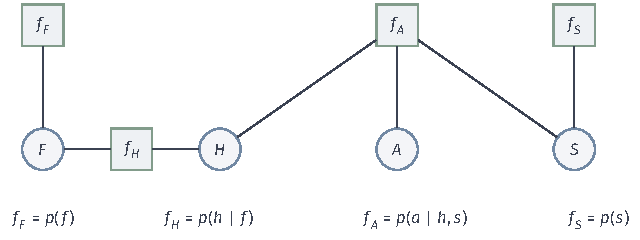
\includegraphics[width=108.433mm]{figures/06-probabilistic-graphical-models/01-representation/tikz/pgm-representations-alarm-factor-graph/figure.pdf}
  \caption{报警模型的四因子表示。圆形表示随机变量，方形表示局部条件分布或先验函数；$f_H$使用$F,H$，$f_A$使用$H,A,S$，连线记录函数的输入变量。}
  \label{fig:pgm-representations-alarm-factor-graph}
\end{figure}

Markov网络的每个势也对应一个因子节点，连接所有作用域变量。边势和一元势可以各自保留为小因子，无需预先合成极大团表。将每个因子的输入变量两两连接，又可得到无向变量图；该图记录共同作用域，但不再区分它由多少个局部函数组成。

三个二元势相乘的$g=\psi_{\{1,2\}}\psi_{\{2,3\}}\psi_{\{1,3\}}$生成一个无向三角形，一般三元势$\psi_{\{1,2,3\}}$也对应同一个团。前者明确分为三个二元函数，后者可能包含不可约的三元作用。三角形本身没有条件独立性来区分两种表示，因子图却显示了局部函数的数量和阶数。这些额外信息来自输入函数的分解。

\subsection{表示的非唯一性}
\label{sec:pgm-representations-nonuniqueness}

合并局部函数会改变因子图，而整个函数可以保持原样。图~\ref{fig:pgm-representations-factor-grouping}将三个二元因子相乘为一个三元因子，六边环随之变成星形。星形虽无环，中心表却从单个二元因子的$r^2$项变为$r^3$项。计算开销因此需要同时看连接结构与因子大小。

\begin{figure}[htbp]
  \centering
  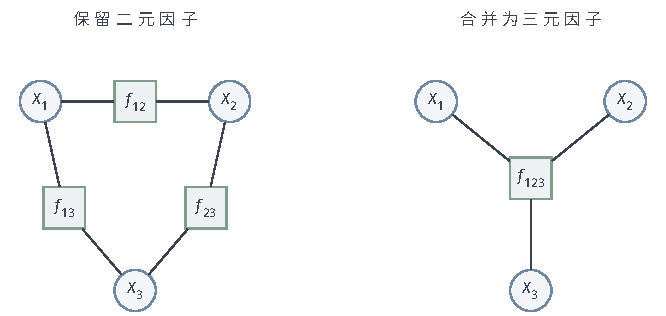
\includegraphics[width=112.000mm]{figures/06-probabilistic-graphical-models/01-representation/tikz/pgm-representations-factor-grouping/figure.pdf}
  \caption{合并因子前后的同一联合函数。左图由三个二元因子构成环，右图以$f_{123}=f_{12}f_{23}f_{13}$形成一个三元因子的星形。两种因子图都生成三角形变量图，局部表规模与连接结构不同。}
  \label{fig:pgm-representations-factor-grouping}
\end{figure}

函数相乘可以合并，能否拆分则要看函数值。若二元函数可以写成两个一元函数的乘积，即满足
\[
  f_{12}(x_1,x_2)=u(x_1)v(x_2),
\]
它的离散函数表就是外积，秩至多为$1$。式~\eqref{eq:pgm-representations-cycle-potentials}的表$\left(\begin{smallmatrix}2&1\\1&2\end{smallmatrix}\right)$行列式为$3$，无法写成两个一元函数的乘积。三元势拆成三个二元势时，同样需要核验具体函数是否具有相应结构。

共享变量还允许在两个因子间转移权重，同时保持总乘积。这种\term{重新参数化}（reparameterization）可以保留原作用域。例如用严格正的$h(x_2)$定义
\[
  \widetilde f_{12}=f_{12}h(x_2),\qquad
  \widetilde f_{23}=\frac{f_{23}}{h(x_2)}.
\]
两新因子的$h$恰好约去，总乘积与原来相同。若仅将一个因子乘以正常数，未归一化函数$g$便同比缩放，调整$Z$后仍得到同一分布$p$。前一种变换保留联合函数，后一种保留归一化分布，二者的代数要求不同。

变量节点的删除也能从因子图读出一些独立性。设$A,B,S\subseteq V$两两不交，$A,B$非空。对非负概率因子分解，删除\emph{变量节点}$S$后，若$A$与$B$分处不同连通分量，给定$\bm{X}_S=\bm{s}$便可按分量整理乘积，并分别归一化，得到$\bm{X}_A\perp\bm{X}_B\mid\bm{X}_S$。运算使用条件分布有效的$\bm{s}$；有限离散情形要求$p(\bm{X}_S=\bm{s})>0$。该分离提供充分保证，具体函数还可能隐含其他独立性。

报警因子图一直有连接$H-f_A-S$，函数却满足$\sum_a f_A(h,a,s)=1$，消去报警后，两原因仍然边缘独立。这条条件归一化等式保留在函数内，拓扑没有显示它。因子图适合据作用域安排计算；碰撞关系仍需原有向图的条件语义，无向Markov约束则由相应变量图的分离判断。

\subsection{因子图上的局部计算}
\label{sec:pgm-representations-local-computation}

有了因子图，就可以在它上面组织推断计算了。本章只说明最基本的局部操作如何由图的连接决定，具体的消元顺序选择、复杂度分析和消息复用留给第~\ref{chap:pgm-elimination}章与第~\ref{chap:pgm-junction-tree}章。先从最常见的问题说起：观测到一部分变量后，想求另一部分（查询）变量的后验分布，就要把既未观测、也不查询的变量全部求和消去。下面的局部计算采用有限离散取值变量和有限个非负实值因子，乘积可以归一化为合法分布。所给证据满足$p(\bm X_S=\bm s)>0$。这些条件保证下面的求和都是有限和，后验归一化分母为正，有限候选集上的最大值也能取得。一般函数的因子图定义本身不要求变量离散；连续查询还需另行处理积分、条件密度版本以及最大值是否取得，不能仅靠下述有限运算公式得到这些保证。

观测$\bm{X}_S=\bm{s}$后，将相关因子中的证据坐标固定在该值。以$Q\subseteq V\setminus S$为查询集，其他待消变量组成$R=V\setminus(Q\cup S)$。将它们求和消去，得到查询的未归一化边缘函数：
\begin{equation}
  \widetilde p(\bm{x}_Q,\bm{s})
  =\sum_{\bm{x}_R}
  \prod_{\alpha\in\mathcal{F}}
  f_\alpha(\bm{x}_{D_\alpha\setminus S},\bm{s}_{D_\alpha\cap S}).
  \label{eq:pgm-representations-marginal-query}
\end{equation}
若$p(\bm{s})>0$，对$\bm{x}_Q$求和得到的常数可将$\widetilde p$归一化，得到后验边缘分布。

分配律使每步计算可以只处理相关因子：$u$不含$x_i$时，有$\sum_{x_i}u\,v=u\sum_{x_i}v$。因此，收集与$x_i$相连的因子，相乘再求和，将所得新函数接到剩余作用域即可。式~\eqref{eq:pgm-representations-cycle-message}就是将两个边因子经消元变为$\{1,3\}$上的新因子。连接关系由此给出每步的输入函数及输出变量集。

求后验边缘回答的是“各状态分别有多可能”，但很多实际问题要的不是概率，而是“最可能的完整情形是什么”：如图像分割中要给出一整幅最可能的标签配置，故障诊断中要给出一组最可能的状态。这时汇总未知变量的算子要从“求和”换成“取最大值”。寻找全部非证据变量的最可能联合配置时，改对其完整配置取最大值：
\[
  \max_{\bm{x}_{V\setminus S}}
  \prod_{\alpha\in\mathcal{F}}f_\alpha.
\]
该查询称为\term{最可能解释}（most probable explanation, MPE）。$Z$对所有候选配置相同，最大化未归一化权重就能比较候选；每步记录取得最大值的状态，结束后回溯，才能恢复最优配置。若仅对部分变量求最优，其他未观测变量需先求和，则形成\term{边缘最大后验推断}（marginal maximum a posteriori inference, marginal MAP）问题。沿用查询集$Q$与其余待消集$R$，它寻找的是
\begin{equation}
  \bm x_Q^\star\in
  \argmax_{\bm x_Q}\left\{
    \sum_{\bm x_R}
    \prod_{\alpha\in\mathcal F}
      f_\alpha(\bm x_{D_\alpha\setminus S},
        \bm s_{D_\alpha\cap S})
  \right\}.
  \label{eq:pgm-representations-marginal-map}
\end{equation}
内层求和汇总没有被选作优化目标的变量，外层最大化再选择查询配置；证据的归一化常数不随$\bm x_Q$改变，所以不影响这个选择。边缘概率查询输出每个查询配置的后验概率，MPE输出全部非证据变量的最优联合配置，边缘MAP则输出查询变量的最优配置。这三个任务保留和消去的信息不同。

边缘MAP混合求和与最大化，两种算子的先后次序会影响结果。用一个人工构造的严格正二元概率表即可看出差别：以$x=0,1$为行、$y=0,1$为列，取
\[
  \bigl[p(x,y)\bigr]=
  \begin{pmatrix}
    0.36&0.04\\
    0.30&0.30
  \end{pmatrix}.
\]
四项之和为$1$，MPE选择最大单格$(x,y)=(0,0)$，概率为$0.36$。若只希望选择$x$，两行的边缘概率分别是$0.40$与$0.60$，边缘MAP便选择$x=1$。先求和再取最大值得到$\max_x\sum_y p(x,y)=0.60$；若颠倒次序，两列最大值相加却得到$\sum_y\max_x p(x,y)=0.36+0.30=0.66$。后一个计算允许第一列选$x=0$、第二列选$x=1$，不再要求同一个$x$配置解释全部$y$状态，因此改变了原查询。

一般混合查询不能任意交换这两个算子，但作用域相互分开时可能提前处理某个最大化。例如固定其余变量$\bm z$后，若乘积为$h(x,\bm z)u(y,\bm z)$，非负性使
\[
  \max_x\sum_y h(x,\bm z)u(y,\bm z)
    =\bigl[\max_x h(x,\bm z)\bigr]
      \bigl[\sum_y u(y,\bm z)\bigr].
\]
这里$h$不含$y$、$u$不含$x$，所以$x$的最佳选择不随被汇总的$y$改变。是否合法换序，要检查当前相关因子的作用域；一个通用的正确顺序是先消去全部$R$，再最大化$Q$，具体图结构可能允许更多安排。

边缘概率查询和完整配置MPE都用乘法组合函数，区别在于汇总状态的算子：\term{和积}（sum-product）随后求和，\term{最大积}（max-product）随后取最大值。在四环的式~\eqref{eq:pgm-representations-cycle-message}中，将求和换为最大化，两端相同时得到$4$，不同时得到$2$；原来的求和结果则为$5$和$4$。输入因子相同，消元算子决定了当前函数回答的是概率汇总还是最优权重。边缘MAP同时使用两种汇总，仍需保留刚才说明的顺序约束。

和积与最大积两套计算的步骤几乎完全相同：都是收集相邻因子加以组合，再对待消变量的取值做汇总，唯一区别是组合用乘法、汇总分别用求和或取最大值。既然流程相同，可将其抽象成一种统一形式，使同一套消息传递实现只需替换两个运算就能服务不同查询；这种抽象还能说明“合法重组”依赖哪些代数性质。将组合函数与汇总状态两项操作抽象出来，就得到\term{半环}（semiring）形式：以$\otimes$组合局部函数，以$\oplus$汇总待消变量的不同取值。采用交换半环时，两运算都满足结合律、交换律，$\otimes$对$\oplus$还满足分配律。以$e_\oplus$记$\oplus$的单位元、$e_\otimes$记$\otimes$的单位元，并有吸收关系$a\otimes e_\oplus=e_\oplus$。这组运算条件让收集因子后的消元写成
\begin{equation}
  \begin{aligned}
    h(\bm{x}_{D\setminus\{i\}})
    &=
    \bigoplus_{x_i}
    \ \bigotimes_{\alpha:\,i\in D_\alpha}
    f_\alpha(\bm{x}_{D_\alpha}),\\
    D&=\bigcup_{\alpha:\,i\in D_\alpha}D_\alpha.
  \end{aligned}
  \label{eq:pgm-representations-semiring-elimination}
\end{equation}
在非负实数上，$(\oplus,\otimes)=(+,\times)$就是和积，其$(e_\oplus,e_\otimes)=(0,1)$；最大积用$(\max,\times)$，单位元也为$0$和$1$。取对数后，在$\mathbb{R}\cup\{-\infty\}$上使用$(\max,+)$，有$(e_\oplus,e_\otimes)=(-\infty,0)$，零权重变为$-\infty$。每种运算都具备上述分配关系，所以同样的收集因子、局部消元步骤可以用于相应的纯和积或纯最大积查询\scite{pgm-overview-kschischang2001}。这里每次汇总只有有限项，普通半环的公理已足以支持重组；若要进行无穷汇总或连续积分，还需相应的收敛与交换运算条件。一个固定的交换半环也不会自动消除边缘MAP混用求和与最大化的顺序限制。

一次消元留下剩余变量上的函数，它概括了被消变量对后续计算的影响。沿图传递这样的函数，就是消息传递的基本操作。在无环因子图上，移除一条边将计算分成不重叠的两部分，一侧的消息能汇总该侧全部影响，因而和积可精确求边缘。有环图反复更新消息时，传回的信息可能已包含先前从当前节点发出的影响，两侧不再分离；后文的环置信传播将讨论这一问题。另一种精确组织是先按顺序消元形成大团，再在团之间安排消息。第~\ref{chap:pgm-elimination}章讨论消元顺序与复杂度，第~\ref{chap:pgm-junction-tree}章介绍消息的组织及复用。

\section{本章小结}
\label{sec:pgm-representations-summary}

图转换会同时涉及分布值、独立性声明和计算结构，三者需分别比较。I-map要求图声明属于分布的真实独立性，即$\mathcal{I}(\mathcal{G})\subseteq\mathcal{I}(p)$，D-map方向相反。当前查询的祖先道德图精确复现d-分离，整图道德化通常减少可见的独立性。碰撞结构与无弦四环分别展示两类图完美表示的边界；弦图与父集成团的有向图则可互相保留全部图分离关系。

祖先道德图将查询两侧的因子分开归一化，从而证明d-分离的可靠性。对未分离查询，离散条件表与线性高斯参数的非平凡多项式提供相容分布中的依赖见证，给出这两个模型类的完备性。若一个固定分布的全部独立性都要对应图的d-分离，还需忠实性，将模型类的存在保证加强到该分布的完美映射。

局部函数的重组可以保留完整分布：有向条件因子成为道德图的团势，弦图团势沿完美消元序生成条件表，非弦图则借填充边容纳中间函数。四环的数值计算中，新增边让图少声明一项独立性，原函数却继续满足它。只有允许新条件表各自自由变化，转换后的完整图模型族才更大。

因子图用变量与函数的连接保留输入分解，按查询选择求和或最大化，实现局部组合与消元。同一分布有多种因子图，连接方式和局部函数的阶数共同决定开销。给定因子和查询后，接下来的任务是选择消元顺序，控制中间函数的大小，并复用已完成的局部计算。

\paragraph{扩展阅读}
Koller与Friedman的教材系统比较有向、无向及因子化表示。书中的转换例子可结合本章的三项比较继续阅读：哪些联合概率保持原样，哪些独立性仍由新图保证，以及局部函数的重组怎样影响推断所需的中间表\scite{pgm-koller2009}。

